
\documentclass[12pt]{article}
\usepackage{amsmath}
\usepackage{graphicx}
\usepackage{listings}
\usepackage{dsfont}
\usepackage{appendix}
\usepackage{natbib}
%\usepackage{url}
\usepackage{float}
\setcitestyle{square}
\usepackage{subcaption}
\usepackage{hyperref}
\hypersetup{
    colorlinks,
    citecolor=black,
    filecolor=black,
    linkcolor=black,
    urlcolor=black
}

\allowdisplaybreaks



\usepackage{setspace}
\doublespacing

\usepackage[bottom=2.54cm, top=2.54cm, left=2.54cm, right=2.54cm]{geometry}
\title{Real-time probabilistic forecasts of the 2018 -- 2019 Ebola outbreak in North-Eastern Democratic \\Republic of Congo}
\author{
  CANDIDATE NUMBER
}
\date{\today}

\begin{document}
\maketitle
\noindent
{\bf Word count:}\\
Abstract: 406  \\% 14 + 61 +139 + 167 + 25 \\
Report: 9,505  % 8574 + 40 + 367 + 113 + 12 + 42 + 189 + 168

\begin{abstract}
  {\bf Objectives:} Construct and evaluate probabilistic forecasting models for the 2018--2019 Ebola outbreak in north-eastern DRC on both a national and sub-national level.
  
  \medskip
  
  {\bf Design:} Using publicly available data on daily numbers of reported Ebola cases from the 2018--2019 Ebola outbreak in DRC, we constructed a set of semi-mechanistic forecasting models based on a branching process with a time-varying reproduction number. This class of models is based on offspring distributions, serial intervals and reproduction numbers, with no additional assumption about the disease transmission process. We included models with both Poisson and negative binomial offspring distributions and two methods for forecasting the reproduction number. These methods used the estimated historic evolution of reproduction number and then either forecasted a constant reproduction number or used a forecast based on a Bayesian state-space model with a semi-local trend. We fitted the models both to national-level data for the whole outbreak and for each individual health zone with forecasting horizons up to 28 days. We compared the forecasts from the different models using proper scoring rules and checked the calibration of the forecasts using the randomised Probability Integral Transform. 

  \medskip
  
  {\bf Results:} On the national level we found that a negative binomial distribution was needed for calibrated one-day-ahead forecasts, but that the model with a Poisson offspring distribution and a semi-local trend for the reproduction number was the best model for longer forecasts and could provide calibrated forecasts for a forecasting horizon of nine days. The semi-local trend models could also provide calibrated forecasts for some of the health zones, but for most of the health zones with a large number of cases the models did at best provide a few days of calibrated forecasts. At both the national and the sub-national level, we found that the models with constant reproduction number would normally underestimate the uncertainty in the process and that semi-local trend models are likely to overestimate the uncertainty of the process. 

  \medskip
  
  {\bf Conclusions:}

  Flexible semi-mechanistic models based on a branching process can be used to give calibrated short-term forecasts of the Ebola outbreak in northern DRC on the national level and partly on the sub-national level. The forecasts can be provided in real time to support the outbreak response and can provide  insight to increase our understanding of the outbreak.

  \medskip

  {\bf Keywords:} Ebola, DRC, probabilistic forecasts, mathematical modelling, semi-mechanistic model, calibration, proper scoring rules.

\end{abstract}

\newpage

\tableofcontents

\newpage

\section{Introduction}


Real-time modelling and forecasting of infectious diseases can play a crucial role during disease outbreaks like the ongoing Ebola outbreak in the north-eastern Democratic Republic of Congo (DRC) \cite{heesterbeekModelingInfectiousDisease2015,riversUsingOutbreakScience2019a}. The use of models for Ebola response was pioneered during the previous large Ebola outbreak in West Africa in 2014--2016 \cite{chretienMathematicalModelingWest}. The models developed during and after this outbreak were used both to increase our understanding of the outbreak and to predict the spread of the outbreak. Forecasts were used in the official response planning \cite{whoebolaresponseteamEbolaVirusDisease2014} and to estimate needed bed capacity \cite{camachoTemporalChangesEbola2015}. Disease modelling has also been successfully implemented and used to inform response plans for many other infectious diseases including Zika \cite{kobresSystematicReviewEvaluation2019} and influenza \cite{chretienInfluenzaForecastingHuman2014}. To make effective use of results from mathematical modelling in an outbreak it is of key importance that modelling outputs are integrated into the outbreak response and decision making \cite{riversUsingOutbreakScience2019a}. This means that forecasts need to be available in real time and integrated into the outbreak surveillance information flow. In addition, improved communication and embedding of modelling and modellers into the outbreak response is needed. 

To provide useful information in an outbreak situation, models should be probabilistic so that they assess and incorporate uncertainty into their predictions \cite{funkAssessingPerformanceRealtime2019, weiCalibrationTestsCount2014,heldProbabilisticForecastingInfectious2017,gneitingEditorialProbabilisticForecasting2008}. An understanding of the range of possible outcomes from a model and their associated probabilities is essential for an effective use of modelling results in an outbreak situation since there are both large uncertainties and randomness associated with the disease transmission process and in the necessary reduction of this process to a mathematical model. Once a model has been formulated, it needs to be critically evaluated before use. Evaluations of probabilistic forecasts not only requires us to assess the accuracy of point predictions, but to assess if the model correctly assess its own uncertainty \cite{gneitingProbabilisticForecastsCalibration2007, czadoPredictiveModelAssessment2009}. A model that successfully assesses its own uncertainty is said to be calibrated. We should strive to create well calibrated models which can be updated in real time and that are interpretable and useful during the outbreak response. 

The aim of this report is to describe a framework for flexible probabilistic forecasts for the ongoing Ebola outbreak in north-eastern DRC and to assess the calibration of the resulting models. We will compare different models using proper scoring rules to choose the model that gives the best forecasts, and use these models to explore the epidemiology of the current outbreak. 

\section{Background}
\subsection{2018--2019 Ebola outbreak in north-eastern DRC}

Ebola virus disease (EVD) is an often fatal disease caused by the Ebola virus that is transmitted through close contact with bodily fluids from infected persons \cite{worldhealthorganisationEbolaVirusDisease}. The symptoms start 2 -- 21 days after infection and include fever, vomiting, diarrhoea and in some cases internal and external bleeding.  Risk factors include close contact with or handling of the infected person or their dead body. This has made outbreak response challenging since health-care workers have had a high risk of infection \cite{brainardRiskFactorsTransmission2016}. Another important source of infections have been burial practices that include direct contact with the dead body \cite{brainardRiskFactorsTransmission2016}. There have been over 20 separate Ebola outbreaks since the first recorded outbreak in 1976, with a basic reproduction number, $R_0$, that has normally been between 1.5 -- 3 \cite{whoebolaresponseteamEbolaVirusDisease2014,legrandUnderstandingDynamicsEbola2007} and a case fatality rate that has varied between 10 and 90 percent. Apart from the large outbreak in Western Africa in 2014--2016 which had over 28,000 cases all of the previous outbreaks have had less than 500 cases \cite{worldhealthorganisationEbolaVirusDisease}, making the current outbreak the second largest in history.

The current outbreak in north-eastern DRC started on the 1st of August 2018, when the Ministry of Health in the Democratic Republic of Congo notified the WHO about a new Ebola outbreak in the North Kivu province \cite{worldhealthorganizationEbolaOutbreakDRC2018a}. North Kivu and the surrounding provinces Ituri and South Kivu constitute a populous region in north-eastern DRC which borders both Rwanda and Uganda. In recent history the people in the region have been involved in both the Second Congo War (1998-2003) and the ongoing ``Kivu Conflict''. The Kivu conflict has seen local rebel forces fight against the armed forces of the government. In addition to local forces, a large UN peacekeeping force has been heavily involved in the region. This makes the area very difficult to operate in due to security concerns and the high levels of distrust from local population towards both the central government and international organisations. By the 27th of September 2018, the outbreak had continued spreading and the WHO assessed that the outbreak constituted a very high national and regional risk \cite{worldhealthorganizationEbolaOutbreakDRC2018b}.

The difficult security situation and the distrust from the local community have made the outbreak response very challenging. This has lead to difficulty in tracing contracts, giving vaccinations and treating patients. There have been many episodes of violence directed towards the Ebola responders, which has led to fatalities and multiple stops in the response activities \cite{worldhealthorganizationEbolaOutbreakDRC2018c,worldhealthorganizationEbolaOutbreakDRC2019a}. Despite these difficulties the outbreak has mainly been contained in the region, with only imported cases and no transmission seen in the large city of Goma or across the borders in Uganda and Rwanda. 

During the outbreak, the experimental vaccination rVSV-ZEBOV-GP has been used in a ring vaccination strategy. The vaccine was given under the compassionate use regime and has been evaluated during the outbreak. Preliminary data shows positive signs that this vaccine will provide protection from Ebola \cite{organizationPreliminaryResultsEfficacy2019}. The vaccines have also been given to health-care workers and children. This outbreak has also seen a randomised trial for four proposed medicines to treat Ebola. The trial was terminated on the 12th of August as it was found that two of the four drugs that were included showed a clear effect of reducing mortality from Ebola, especially with early treatment \cite{nationalinstituteofallergyandinfectiousdiseasesIndependentMonitoringBoard2019}.

On the 17th of July the Director General of the WHO declared the Ebola outbreak a Public Health Emergency of International Concern \cite{worldhealthorganizationEbolaOutbreakDRC2019} and as of mid-September 2019 the outbreak is still ongoing with recent new cases from 17 health zones \cite{worldhealthorganizationEbolaOutbreakDRC2019b}. 

\subsection{Mathematical modelling of Ebola}

A large number of different mathematical models have been proposed for modelling and forecasting of Ebola\cite{chretienMathematicalModelingWest,viboudRAPIDDEbolaForecasting2018}. The models can be divided into categories based on their structure: mechanistic, semi-mechanistic, phenomenological and hybrid models. Mechanistic models are based on a specified mechanism for disease transmission and include standard compartmental models, while phenomenological models aim to describe empirical relationships and do not include any specified mechanism for disease transmission. For Ebola prediction, an example of a mechanistic model is the SEIR model in \cite{gaffeyApplicationCDCEbolaResponse2018}. Many different phenomenological models have been developed for Ebola predictions. They include the logistic growth models \cite{pellUsingPhenomenologicalModels2018} and autoregressive integrated moving average models used for many applications of time-series forecasting \cite{mForecastingTrendCases2017}. A semi-mechanistic model includes some mechanistic assumptions, together with some parts of the model that are more empirical or phenomenological. The aim of these models is to model some important parts of the disease transmission process, while giving enough flexibility to fit complicated outbreak histories. For Ebola forecasting, examples include SEIR models with a random walk describing the transmission rate or reproduction number  \cite{funkAssessingPerformanceRealtime2019,asherForecastingEbolaRegression2018}. Based on a review of models for the West African Ebola outbreak, it was found that it was important that models actively included the uncertainty in the disease transmission process \cite{chretienMathematicalModelingWest, kingAvoidableErrorsModelling2015} and that community standards for developing, reporting and comparing models are put in place. 

The most recent evaluation of Ebola models was the RAPIDD Ebola Forecasting challenge in 2018 \cite{viboudRAPIDDEbolaForecasting2018}. The challenge presented a range of different scenarios of a simulated Ebola outbreak that was similar to the West African outbreak, and invited different groups to submit forecasts and compared them. Eleven different models with a large range of different modelling structures were submitted to the competition. When the models were compared, it was found that for short-term forecasting the accuracy was not related to model complexity and that ``light'' non-parametric models achieved similar forecasting accuracy to larger mechanistic models. The more complex mechanistic models would, on the other hand, be better suited to understand the effects of interventions. 

In this thesis we will present a semi-mechanistic modelling framework that includes some mechanistic assumptions about serial intervals and forces of infection combined with flexible time-series methods. The aim is a flexible model with parameters that are easily interpretable and useful during an outbreak response situation. This also requires that the models can be run in real time and integrated with the response surveillance. 

\section{Methods}

\subsection{Data Sources}

We will use daily reports of new cases from the Ebola outbreak in north-eastern DRC as reported by the Ministry of Health in DRC and the World Health Organisation. This data has been made publicly available and has been distributed via the Humanitarian Data Exchange \cite{hummanitariandataexchangeEbolaCasesDeaths}. We use data from the beginning of the outbreak until the 1st of September 2019. The data gives the cumulative number of cases reported every day, which we used to calculate the incident cases both at the national and at the health-zone level. For our models, we will use confirmed cases so that estimates of the reproduction number and other epidemiological parameters correspond only to Ebola and not to Ebola and Ebola-like illnesses. Due to the nature of the outbreak and the nature of the data, some confirmed cases are later found to not be Ebola after all. This can lead to days with negative incidence since the cumulative number of cases used to calculate the incidence has been corrected from an earlier date. We have chosen to set any negative incidence to zero as we do not have any information about which of the earlier cases has been removed. In July and August 2018 there were some days without any reported data. For these days we equally distribute the number of new cases seen at the end of the interval of missing data to each missing day.

\subsection{Ethics}
Since only secondary data fully in the public domain was used, no ethics approval was needed (LSHTM MSc Ethics ref: 16735). 

\subsection{Model}

With our aim of constructing a flexible semi-mechanistic framework for the modelling of Ebola we considered models where the daily incidence, $I_t$, follows a modified branching process~\cite{jacobBranchingProcessesTheir2010}. This class of models has been considered for infectious disease modelling previously in \cite{coriNewFrameworkSoftware2013,lloyd-smithSuperspreadingEffectIndividual2005,nouvelletSimpleApproachMeasure2018} and was used to model Ebola during the 2014--2016 outbreak in Western Africa \cite{whoebolaresponseteamEbolaVirusDisease2014, internationalebolaresponseteamExposurePatternsDriving2016}. The main idea is that each infected person gives rise to $\nu$ new infections, where $\nu$ is a random variable distributed with an offspring distribution with an expected value given by the reproduction number $R$. This gives rise to the standard interpretation of the reproduction number as the average number of secondary cases caused by one primary case. Using random variables for the number of secondary cases gives a stochastic model that allows us to model the inherent uncertainty in the disease transmission process. To model the time between the initial case and the secondary cases, we will use the serial interval. This gives a process where the expected number of new cases at time $t$ is given by the force of infection, $\lambda_t$, which is a product of previous incidence values weighted by the discretised serial interval in days, $w_\tau$, and the instantaneous reproduction number, $R_t$. Here $R_t$ is reproduction number for the infected people who are transmitting the disease at time $t$. The expected value of the incidence at time $t$ is given by

\begin{equation}
  E(I_t) = \lambda_t =  R_t \sum^{t-1}_{s=1} I_s w_{t-s}.
  \label{eq:mean_It}
\end{equation}

This equation gives a general and flexible modelling framework where an individual model is specified by the probability distribution for $I_t$, the serial interval and the reproduction number as a function of time. Due to the semi-mechanistic nature of this model, it does not depend on many assumptions about the disease transmission process. The main assumptions include that the force of infection is given by the weighted sum of incidence and serial interval and that the offspring distribution and time-varying reproduction number can adequately describe the outbreak. For all the models in this study we will use a gamma distribution with a mean of 15.3 days and standard deviation of 9.3 days as the serial interval. This was the serial interval obtained by fitted to data from the West-Africa Ebola outbreak \cite{whoebolaresponseteamEbolaVirusDisease2014}. Our general approach will be to use a few different specifications for the offspring probability distribution and for estimating the time-varying reproduction number and then assess which model gives the best fit to the data.

\subsubsection{Offspring distribution}
The offspring distribution gives the distribution of the number of new infections from each infected person. By definition the expected value of this distribution is the reproduction number. The offspring distribution needs to be a discrete probability distribution over the non-negative integers. The simplest such distribution is the Poisson distribution, where the probability of observing $k$ cases, $P(X=k)$ is given by
\[P(X=k) = e^{-\lambda}\frac{\lambda^k}{k!}, \]
where the $\lambda$ is both the mean and the variance of the distribution. This distribution implies that the number of new infections over a small time interval is described by a constant rate where the chance of a new infection in each small interval is independent.

For a number of diseases it has been shown that the offspring distribution has a larger variance than that given by the Poisson distribution and has so called super-spreaders \cite{lloyd-smithSuperspreadingEffectIndividual2005}. One common way of modelling this over-dispersed distribution is by the negative binomial distribution. The negative binomial distribution describes a process where we have a series of independent opportunities to infect a new person, each with probability, $p$, where the process continues until we have had $r$ infection opportunities without an infection. The distribution is given by

\[P(X=k) = {k + r - 1 \choose k} (1-p)^rp^k, \]

with $E(X)=\frac{pr}{1-p}$ and $Var(X) = \frac{pr}{(1-p)^2}$. We will use a parameterisation of the negative binomial distribution where we use the mean, $\mu$, and the dispersion parameter $k$. In this formulation the variance is given by $\mu + \frac{\mu^2}{k}$, and when $k \rightarrow \infty$ we get back a Poisson distribution. The smaller $k$ is, the more the outbreak is dominated by a few super-spreaders, and the larger $k$ is, the more similar the impact of each infected person. For SARS, it has been found that $k=0.16$ \cite{lloyd-smithSuperspreadingEffectIndividual2005}. For the Ebola outbreak in West Africa, they found $k=0.53$ using conservative assumptions and data from the transmission tree of the infections \cite{internationalebolaresponseteamExposurePatternsDriving2016}. The different offspring distributions can be seen in Figure \ref{fig:offspring}

\begin{figure}[h]
  \centering
  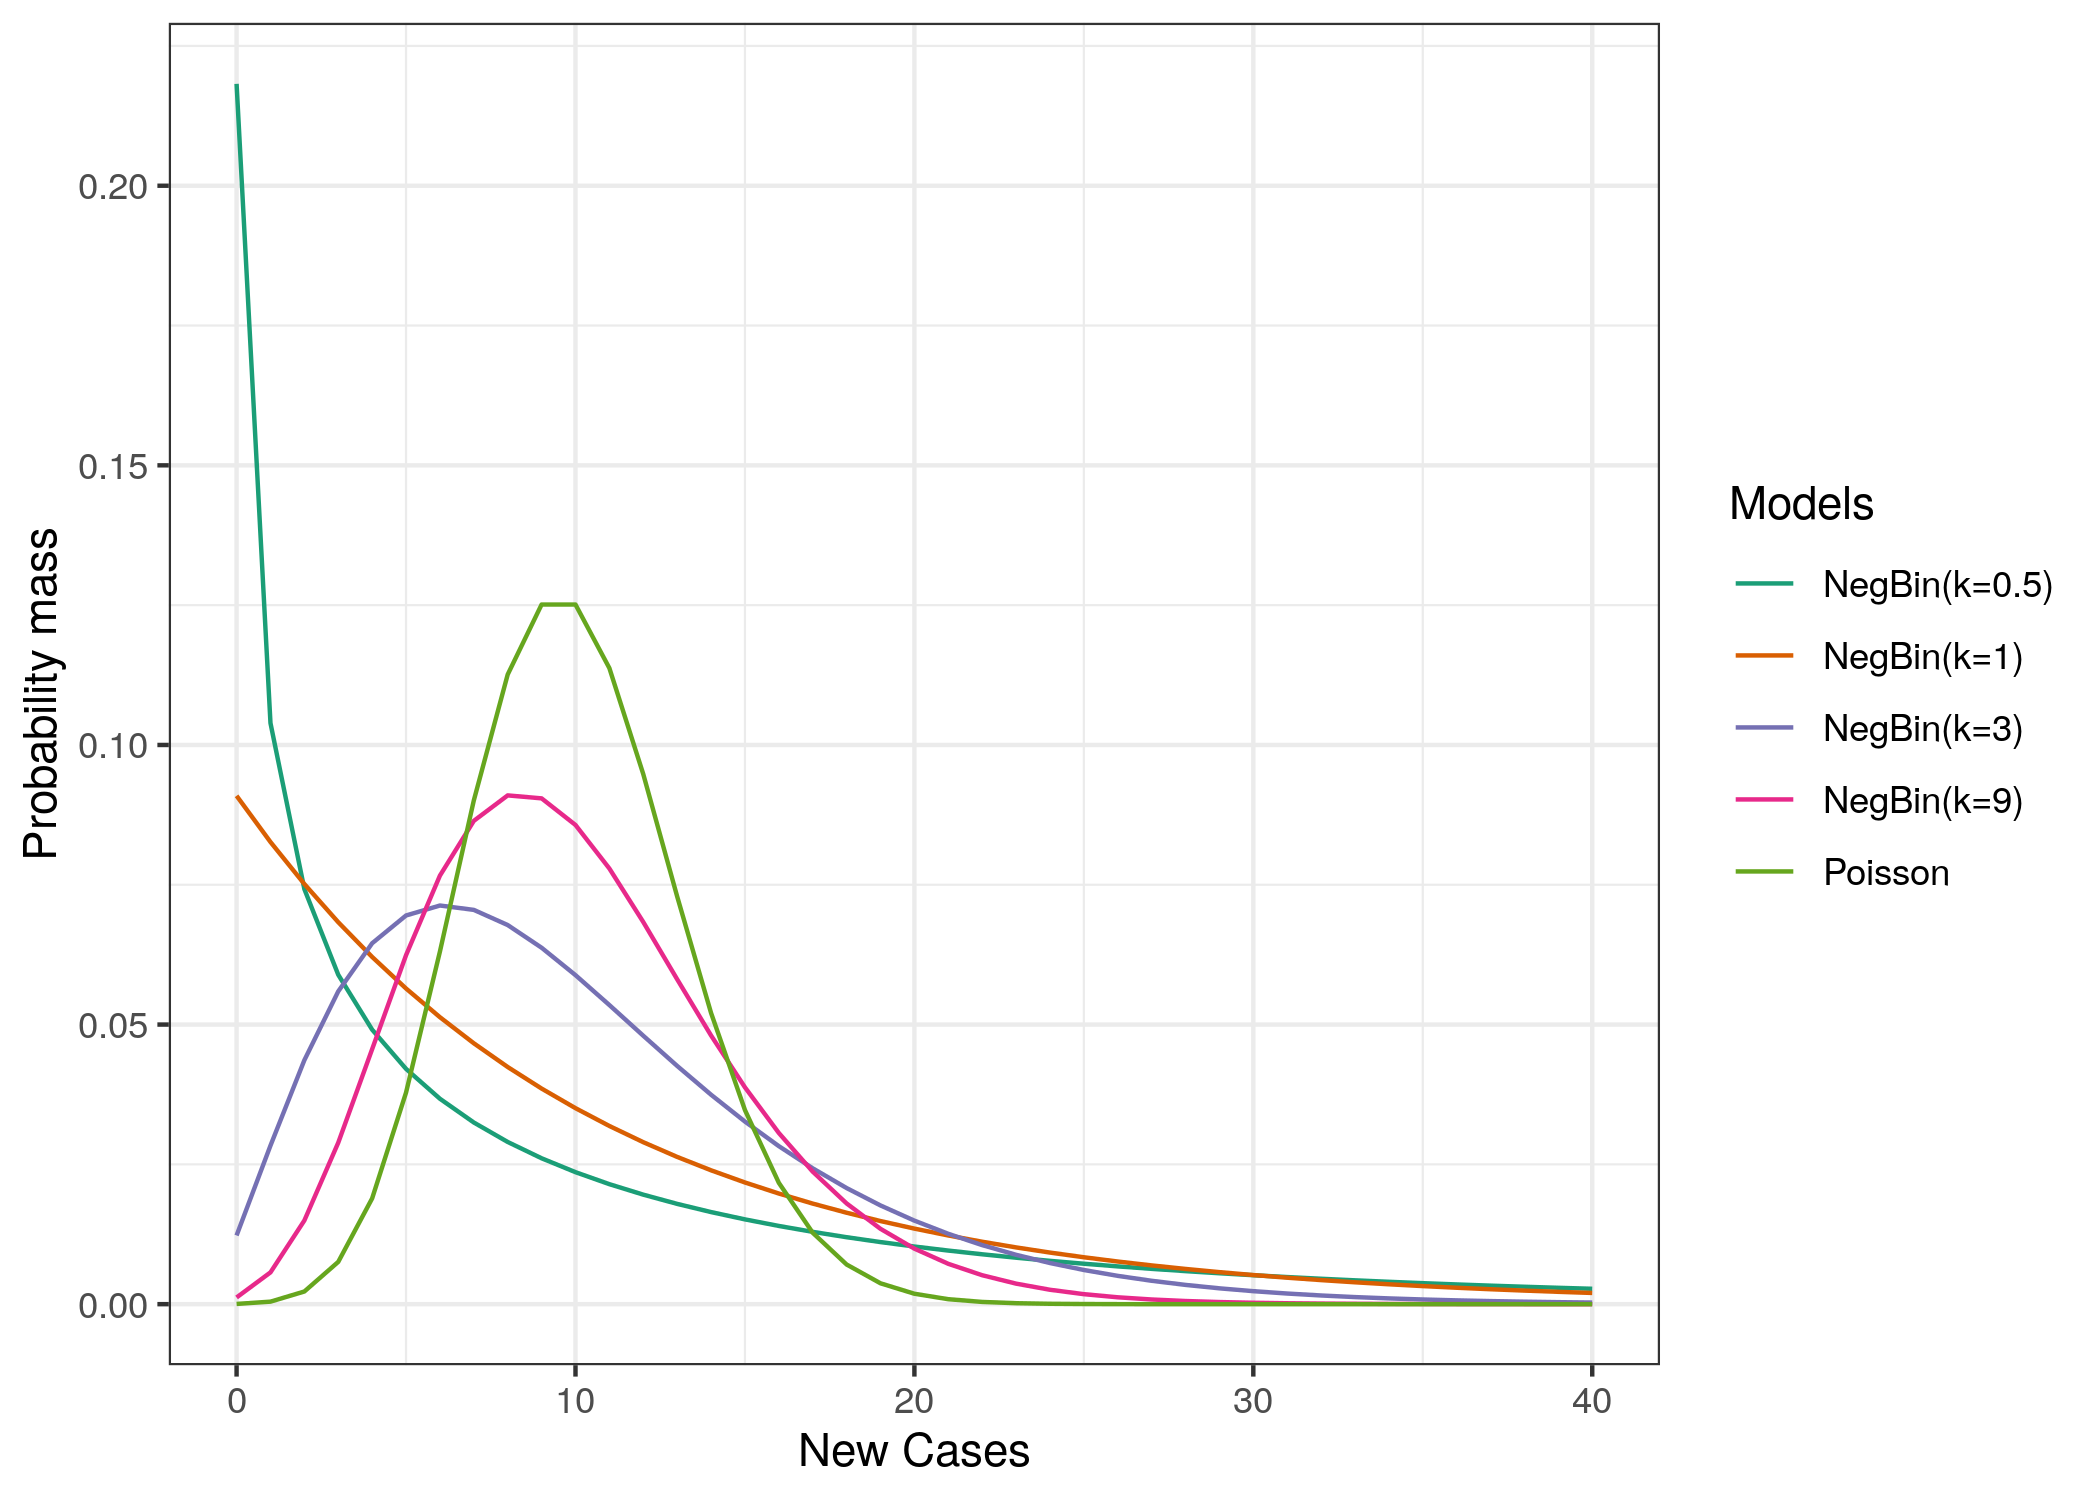
\includegraphics[width=\textwidth]{../output/prob_dist.png}
  \caption{Poisson and negative binomial offspring distributions with a varying dispersion parameter $k$. All the distributions have a mean of 10.}
  \label{fig:offspring}
\end{figure}

The distribution for total incidence is given by the sum of the offspring distributions for each infected person weighted by the serial distribution. For both the Poisson and negative binomial distribution, the sum of independent realisations of the distributions will give back the same distribution with an expected value given by the sum of the expected values. For the negative binomial distribution the dispersion parameter $k$ will remain the same if it is equal for all the realisations. Therefore the probability distribution for incidence is also given by either the Poisson or the negative binomial distribution if the individual offspring distribution is given by one of the two distributions. We will investigate models with both of these offspring distributions to assess which models make better predictions during the current outbreak.

\subsubsection{Reproduction number}
The final ingredient needed to completely specify the dynamics of the model is the evolution of the reproduction number with time. The function for $R_t$ could be modelled as a parametric function where we could fit the parameters to data. Alternatively, we can use non-parametric specification to allow a fairly unconstrained evolution with time, which we choose to do here. This free function for the reproduction number is what gives the model its flexibility to fit a large number of outbreak types. As is common for other non-parametric methods, we will impose conditions on the rate of change of the reproduction number with time to ensure that the evolution of the reproduction number is sensible and not jumping around too much, in order to avoid overfitting.

%%The model could for example reproduce in expetation a standard compartmental model where the reproduction number is given by $R(t) = R_os(t)$, where $s(t)$ is the fraction of susceptibles. In a normal SIER model with a constant rate to move between the ``E'' and the ``I'' compartment the serial interval woudl be exponential distributed.

To forecast $I_t$, we first need to forecast $R_t$ from data prior to $t$. In this study we will use an approach where to forecast $R_t$, we first estimate the values of the reproduction number prior to $t$ using the method described below. We then use these estimated values to predict the future evolution of $R_t$. To estimate the reproduction number from the historical incidence data, we use the method developed in \cite{coriNewFrameworkSoftware2013,thompsonImprovedInferenceTimevarying2019}. This approache used the same formulation as in Equation \ref{eq:mean_It} to estimate the reproduction number from daily incidence. If the reproduction number is estimated daily, it is likely to vary too much from day to day in a manner that is unrealistic. Therefore the method averages over the last 7 days to get more stable estimates. A Bayesian procedure is used to estimate both the best fit value and the credible region of the estimate. We use the R-package EpiEstim \cite{coriEpiEstimEpiEstimPackage2013} to estimate the reproduction number using a parametric gamma distribution for the serial interval with the mean of 15.3 days and a standard deviation of 9.3 days \cite{whoebolaresponseteamEbolaVirusDisease2014}.

Once we have calculated the historical values of $R_t$, we can use them to calculate a forecast for $R_t$ that can be used for predictions of new incidence. We will use two different procedures to forecast the reproduction number. The first method is a simple method were we assume that the reproduction number remains constant from the last historical value. We use the uncertainties given by the method in \cite{coriNewFrameworkSoftware2013} as a prediction interval. In practice this means that to predict the value of $R_t$, we use the method above to find the parameters of the posterior distribution for $R_{t-1}$. We then get realisations of $R_t$ by drawing random numbers from this posterior distribution. When we use a gamma-prior distribution and have no uncertainty in the serial interval parameters, the posterior distribution is also a gamma distribution  \cite{coriNewFrameworkSoftware2013}.

The second approach to forecast the reproduction number is based on Bayesian structural time series model fitted to the historical values of $R_t$. We use a model with a semi-local linear trend to allow the estimation of a trend in the recent data. To ensure that predicted values of $R_t$ are between 0 and 15, we fit the time series on a transformed scale

\begin{equation}
r^*_t = log\left(\frac{R_t}{15 - R_t}\right).
\label{eq:transform}
\end{equation}

We use the R-package BSTS \cite{scottBstsBayesianStructural2019} to fit the Bayesian structural time series with the following model:

\[r^*_{t+1} = r^*_t + \delta_t + \epsilon_t, \epsilon_t \sim N(0, \sigma_\mu),\]
\[\delta_{t+1} = D + \phi(\delta_t - D) + \eta_t, \eta_t \sim N(0, \sigma_\delta).\]

$\delta_t$ is the semi-local trend that we model as an auto-regressive process of order one. This gives a trend process that can oscillate around the level $D$ with smaller random-walk excursions. Inverse gamma-priors are used for the standard deviation parameters $\sigma_\mu$ and $\sigma_\delta$, a Gaussian prior on $D$ and a normal $N(0, 0.1)$ prior for $\phi$ that is truncated at -1 and 1. The $\phi$ parameter determines how much the trend behaves as a random walk. For $\phi=1$ the trend follows a random walk, while for $\phi=0$ the trend is just constant with Gaussian noise. We use a regularising prior for small values of $\phi$ to keep the model from overfitting by e.g having a very rapid growth in the variance of $r^*$ that would make the model very over-dispersed. A Markow Chain Monte Carlo (MCMC) algorithm is used to estimate the parameters in the model which then allows us to forecast future values of $r^*$. After the model is fitted for all the values up to  $r^*_{t-1}$, we can draw samples of the predictive distribution for $r^*_t$. After using the inverse transform of Equation \ref{eq:transform} to get predictions for $R_t$, we can use these values to forecast incidence. 


\subsubsection{Forecasting incidence}

Once we have specified our model by specifying the offspring distribution and the method for forecasting $R_t$, we can use the model to generate probabilistic forecasts. As in many other applications, the forecast is not available in a closed form, but we can simulate the model to get a sample of values from the predictive distribution. If we want to generate a forecast for $I_{t}$, we first use all the data up until and including time $t-1$ to estimate the history of the reproduction number until time. Our probabilistic forecast will be based on sampling possible outcomes to generate a distribution of outcomes. We therefore first draw a sample for $R_{t}$ from the predictive distributions of the models discussed above, and then combine this with the historical incidence data to calculate the total force of infection $\lambda_{t}$. We then sample $I_{t}$ from the specified offspring distribution with an expected value given by $\lambda_{t}$ (Equation \ref{eq:mean_It}). The procedure is repeated many times to build up the predictive distribution. If we want to forecast over multiple time steps, we follow the same procedure by sampling values for the reproduction number for $t+1$. When calculating $\lambda_{t+1}$, we use the sampled value for $I_{t}$ together with the historical data prior to $t$. This procedure can easily be iterated to allow forecasts for any forecasting horizon.


\subsection{Assessing probabilistic forecasts}

The aim of probabilistic forecasts is not only to predict the correct average value, but to forecast the correct probabilities for all the different possible outcomes. Therefore, when evaluating such forecasts, it is not sufficient to use metrics that only depend on a point estimate like the mean or median, such as the mean absolute error. To assess the forecasts of the models discussed in the previous section, we will follow the paradigm of maximising sharpness of the predictive distribution subject to calibration \cite{gneitingProbabilisticForecastsCalibration2007}. In addition we will consider proper scoring rules for comparing probabilistic forecasts. We follow the approach taken in \cite{funkAssessingPerformanceRealtime2019}, where probabilistic forecasts for the West African Ebola outbreak were assessed using similar methods.

\subsubsection{Calibration}
A forecasting model is calibrated if the forecasted distribution is equal to the actual distribution of observed values. This means that the model can accurately assess its own uncertainty. For example, a well calibrated model that predicts that it will rain with a 60\% chance should see that on average it does rain on 60\% of those days. Mathematically, if we assume that the real distribution of outcomes in nature is given by a cumulative density function, $G_t$, and our model predicts a cumulative density function, $F_t$, we say that the forecast is ideal and therefore perfectly calibrated if $F_t=G_t$. To assess calibration, we will use a randomised Probability Integral Transform (PIT) \cite{czadoPredictiveModelAssessment2009a}. We consider a forecasted cumulative distribution, $F_t$, compared to an observed value $k_t$. For each such pair of forecast and observed value we calculate
\[ u_t = F_t(k_t) + \nu (F_t(k_t) - F_t(k_t -1)),\]
where $\nu$ is a standard uniform random variable. If the prediction is ideal, the values $u_t$ will be distributed as a standard uniform distribution. Once we have calculated a set of $u_t$ values, we can then use the Anderson-Darling test of uniformity to assess if the distribution of $u_t$ is uniform. If the p-value for this test is less than 0.1, we find that there is evidence that the model is not calibrated, following the suggestion in \cite{funkAssessingPerformanceRealtime2019}. We implement this using the goftest \cite{farawayGoftestClassicalGoodnessofFit2017} R-package. It is important to note that uniform PIT values are a necessary but not sufficient condition for an ideal forecast and that since we only have limited data, we might not be able to reject calibration even if the model is not well calibrated. In addition to assessing calibration, a histogram of PIT values can tell us if the forecast is under or over-dispersed \cite{czadoPredictiveModelAssessment2009a}. If the forecast is too dispersed (i.e. uncertainty is overestimated), the PIT values are likely to cluster at the centre of the PIT histogram, while if the forecast is under-dispersed (i.e uncertainty is underestimated), they are likely to cluster along the edges of the histogram. We introduce a simple measure of centrality, which is equal to the fraction of $u_t$ values that are between 0.25 and 0.75 as a way to assess if the forecasts are under or over-dispersed if they are not calibrated
\[\text{centrality} = \frac{\text{Number where }0.25 < u_t < 0.75}{\text{Total number}} - 0.5.\]
When the centrality score is less than 0, most of the PIT values are outside of the central region, suggesting that the forecasts are underestimating the real uncertainty.  If the centrality score is larger than 0, then the PIT scores are mainly in the central region and this indicates that the forecasts are overestimating the amount of uncertainty. Since the PIT values include a random component, we will  repeat the calculations of the PIT values 30 times for each set of forecasts and take averages to average out the effect of the randomness in the definition of $u_t$.

\subsubsection{Sharpness and bias}
Sharpness is defined as the range of values in the forecast. The sharper a forecast, the more certain the model is of the predicted values. Sharpness depends only on the forecast and not on the observed values. We will use the normalised absolute deviation about the median of $I_t$ to quantify sharpness

\[ S(I_t) = \frac{1}{0.675} \text{median}(|I_t - \text{median}(I_t)|),\]
where the normalisation factor means that $S$ is equal to the standard deviation if $F_t$ is normal.

It is also of importance to assess the bias of the forecast which indicates if we are more likely to predict too large or too small values. Following \cite{funkAssessingPerformanceRealtime2019}, we will quantity bias as
\[B_t(F_t, k_t) = 1 - (F_t(k_t) - F_t(k_t - 1)).\]
If $B_t=0$, half the probability mass is above and half below the observed value, and the forecast is unbiased. $B_t$ is always between -1 and 1, with both extreme values signifying a completely biased forecast where all the forecasted values are either smaller or larger than the observed value.

\subsubsection{Proper scoring rules}
Proper scoring rules have been developed to compare and rank probabilistic forecasts \cite{gneitingStrictlyProperScoring2007}. To be a proper scoring rule, the scoring rule has to be minimised when the forecast is ideal. These scoring rules combine calibration and sharpness and give a consistent ranking of forecasts. We will use the ranked probability score (RPS) and the Dawid-Sebastiani score (DSS) as implemented in the scoringRules R-package \cite{jordanEvaluatingProbabilisticForecasts2018} for samples from the predictive distribution. The RPS score is given by 
\[RPS(F_t,k_t) = \sum_{i=0}^\infty(F_t(i) - \mathds{1}(i \geq k_t))^2, \]
and can be viewed as an extension of the mean absolute error for a deterministic forecast. The DSS score only depends on the mean, $\mu_p$, and standard deviation, $\sigma_p$, of the predictive distribution
\[DSS(F_t, k_t) = \left(\frac{k_t- \mu_p}{\sigma_p}\right)^2 + 2\log\sigma_p.\]
The DSS allows an intuitive understanding of the proper scoring rules. The first term tells us about how far away the observed value is from the mean of the predictive distribution in units of the standard deviation, and the second term gives information about the sharpness of the predictive distribution. For our models, we will only have samples from the predictive distribution. To calculate the RPS, a kernel density estimate is used to estimate $F_t$, and for the DSS we use the mean and standard deviation of the sample. 

\subsection{Implementation}
All the models and assessments were implemented in the R programming language \cite{rcoreteamLanguageEnvironmentStatistical2018} and are available as open-source code at \cite{LinkSourceCode}. We will consider four different models to assess which model provides the best forecasts. The models are:

\begin{enumerate}
\item{Model 1 (Poisson Latest): Constant reproduction number and Poisson offspring distribution}
\item{Model 2 (NegBin Latest): Constant reproduction number and negative binomial offspring distribution}
\item{Model 3 (Poisson Semi-local): Varying reproduction number with a semi-local trend and Poisson offspring distribution}
\item{Model 4 (NegBin Semi-local): Varying reproduction number with a semi-local trend and negative binomial offspring distribution}
\end{enumerate}

To determine the dispersion parameter $k$ for the negative binomial models, we find the value that minimises the ranked probability score for the one-day-ahead predictions for the model at the national level for the simple negative binomial model (Model 2). We run the models both on the national level using data from the entire outbreak and on the sub-national level. For sub-national predictions, we run the model on each health zone separately, using only data from that health zone. This corresponds to an assumption that once a case has been imported into a health zone, the outbreak in the health zone is independent of the rest of the outbreak. 

To evaluate a model, we will estimate the calibration, sharpness, bias, DSS score and RPS for daily forecasts with forecasting horizons up to 28 days. To do this, we start 17 days~\footnote{The 17 days are due to the fact that the method for estimating the reproduction number only starts providing estimates of the reproduction number after a number of days that is equal to the mean of the serial interval plus one. Since we used a serial interval with mean 15.3, this gives 17 days.} after the first case of the outbreak in the given location and calculate the $d$-days-ahead prediction for all historically available data. For the calibration, we use all forecasts for the $d$-days-ahead forecasts compared to the observed values to assess if PIT values are uniformly distributed, while for all the other metrics we average them over all the available start days for the forecast.

To evaluate the overall quality of the health zone forecasts, we first combine the calibration and scores from each health zone. For the proper scoring rules, sharpness and bias, we average the $d$-day-ahead prediction scores over all the health zones, and for the centrality and calibration based on the randomised PIT, we combine all the $u_t$ values from all the health zones and calculate one combined centrality and calibration score for each $d$-day-ahead prediction. In addtion we evaluate the health zone forecasts by adding up the predictions from each health zone and compare that to the national-level data.

\section{Results}

A total of 2,926 confirmed Ebola cases and 1,926 confirmed Ebola deaths have been reported in the ongoing outbreak in DRC as of the 31st of August 2019, giving a case fatality ratio of 66\%. Figure \ref{fig:epi_curve} shows the weekly number of confirmed cases and the map in Figure \ref{fig:tot_map} shows the total number of cases from each health zone. From Figure \ref{fig:epi_curve} and the estimate of the instantaneous reproduction number in Figure \ref{fig:rep_num}, we can see the evolution of the outbreak. After the initial period with varying weekly case numbers, there was an increase in cases from October 2018 with a large reproduction number, followed by a more varied period where the reproduction number stayed around 1 with some waves of larger weekly incidence around December 2018 and February 2019. From late March and early April 2019, the number of cases per week increased significantly as the reproduction number rapidly increased to over 2. The larger number of weekly cases continued in June and July even as the reproduction number decreased. From July 2019 the reproduction has returned to around one, indicating that the outbreak is still not under control, but that the intensity of the outbreak is less than in May and June. There are large regional differences in the number of cases. Beni and Katwa health zones have been hardest hit sharing close to half the cases between them. From the epi-curve there seems to be some connection between the large increases in incidence and introduction or reintroduction of Ebola into specific health zones. The outbreak started mainly in Mabalako, then in October 2018 the peak was due to increased transmission in Beni, while the peak of incidence in February 2019 was mainly dominated by cases in the health zone of Katwa. The large increase of cases starting around March/April saw an increasing number of health zones reporting new cases. From this it is clear that the hot spot of the disease is moving from health zone to health zone.

\begin{figure}[h!]
\begin{subfigure}{0.48\textwidth}
  \centering

  % include first image
  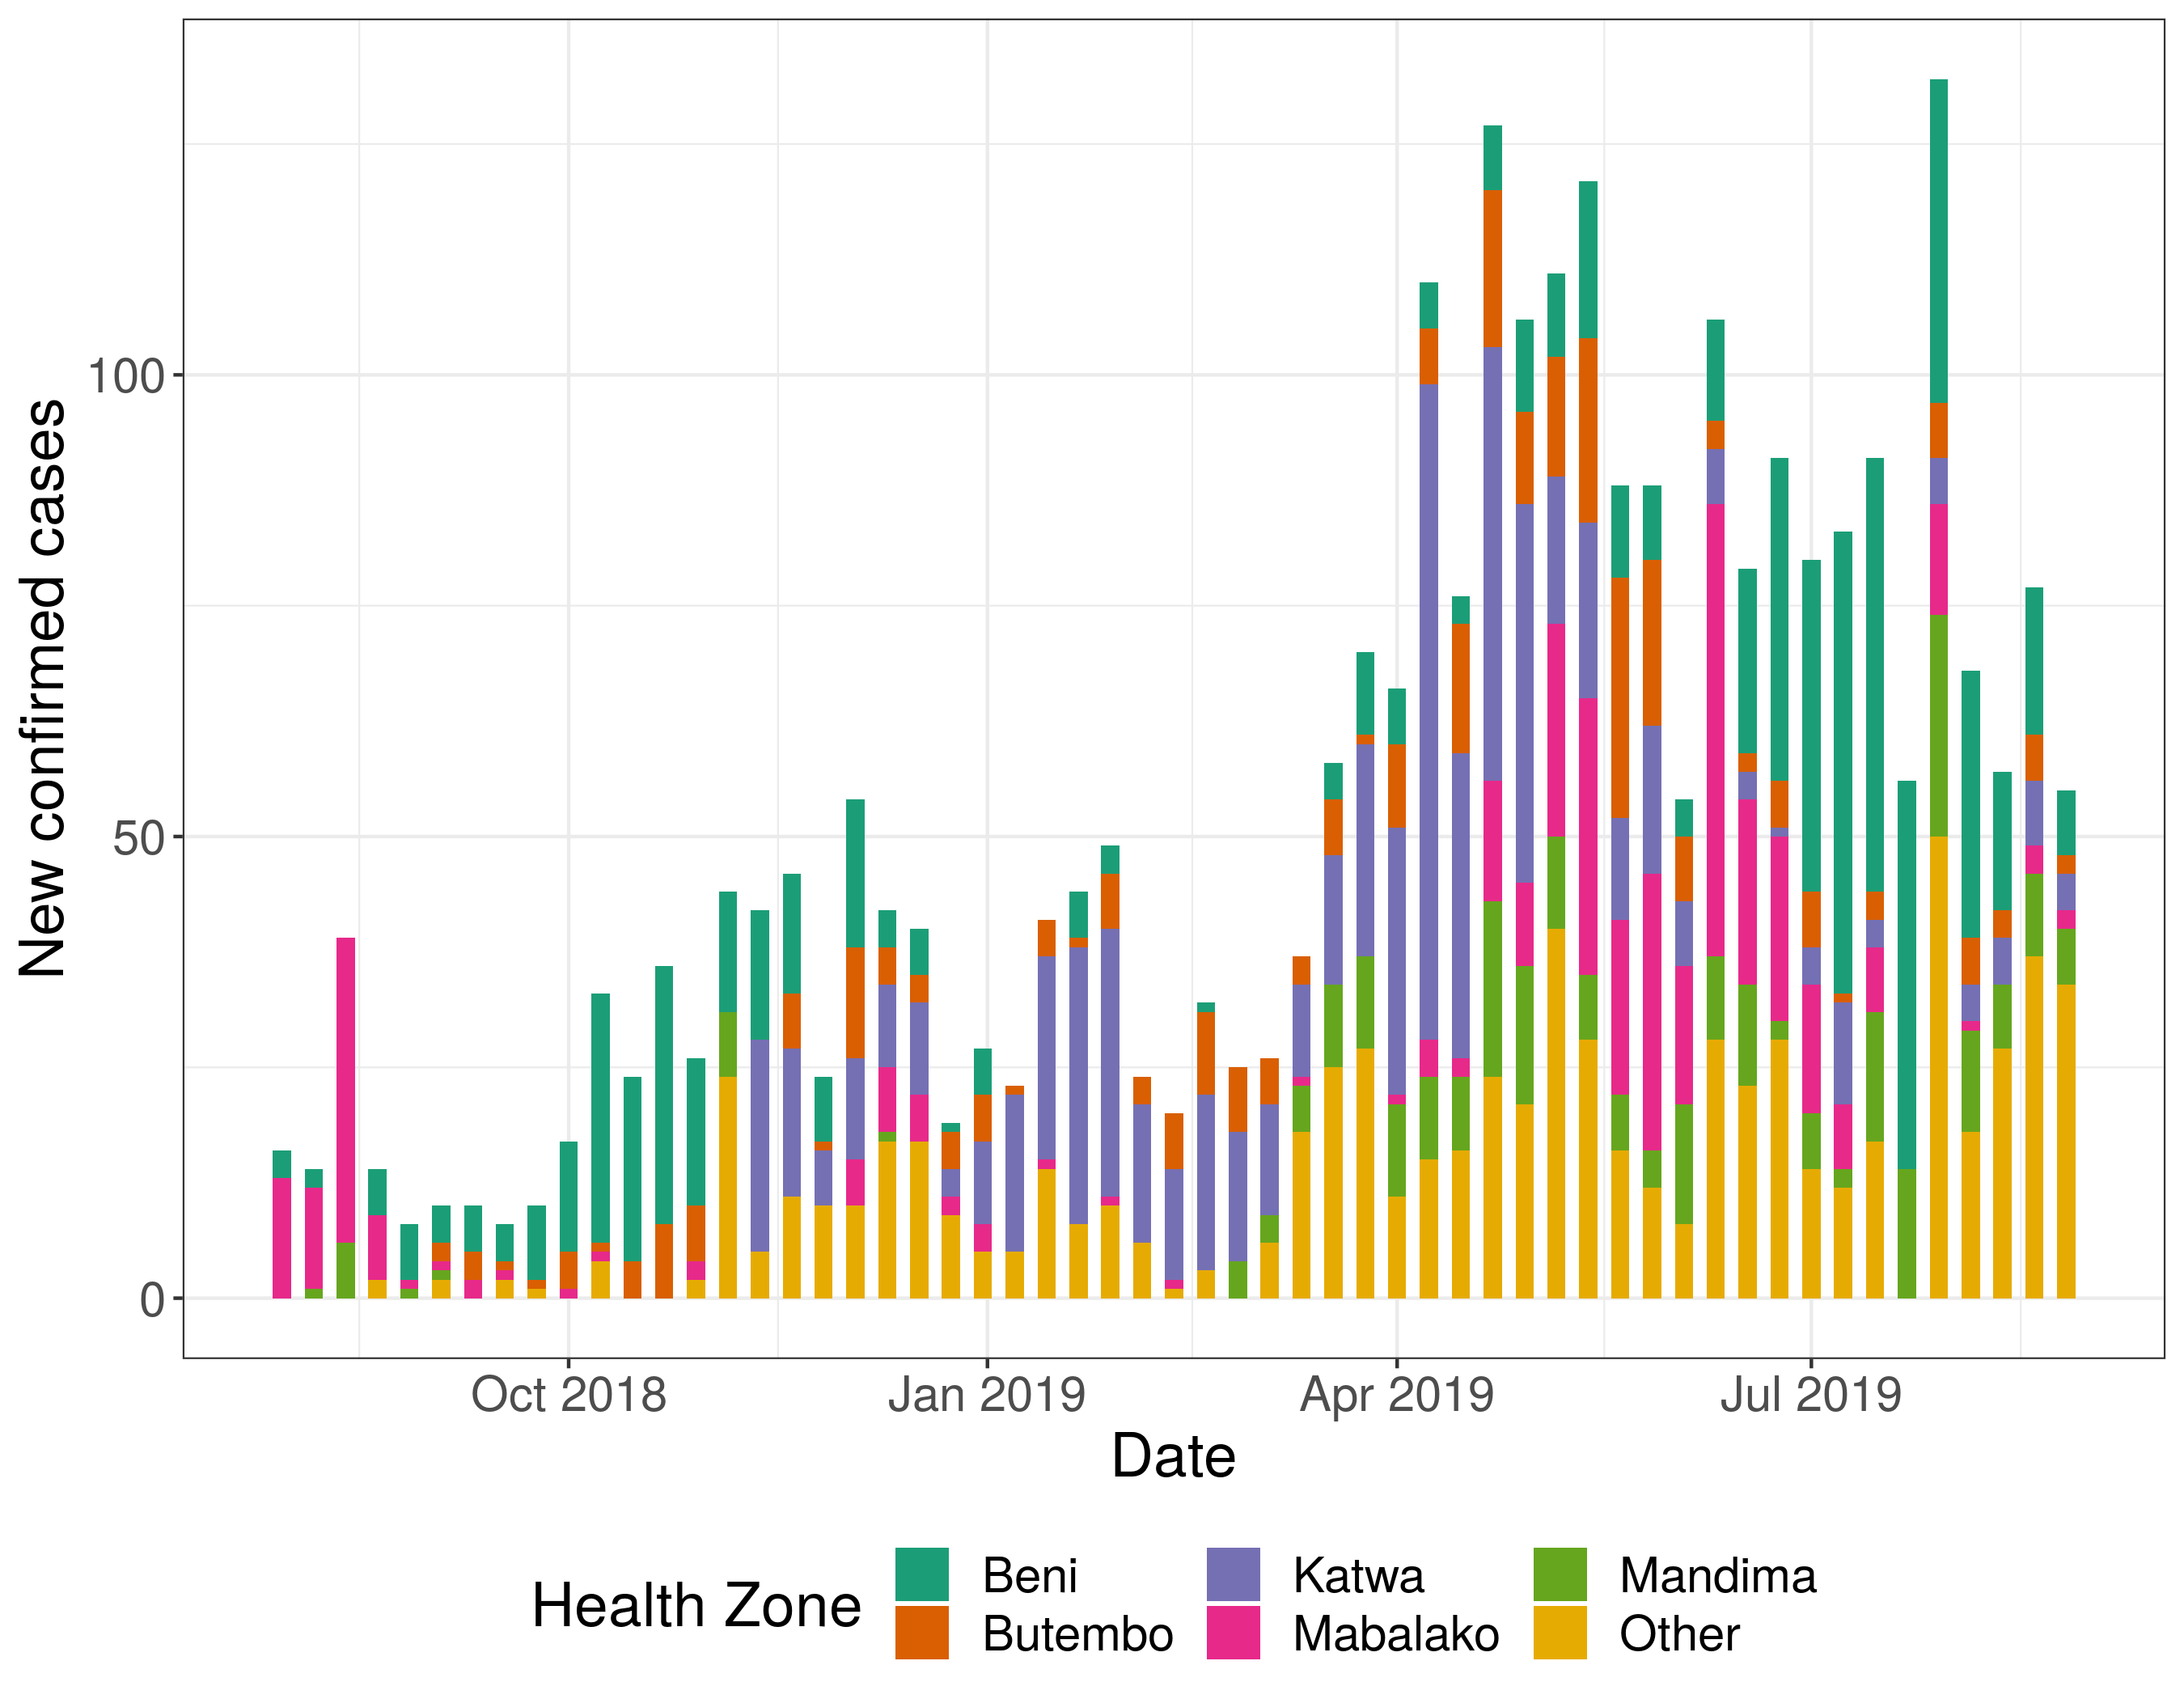
\includegraphics[width=\textwidth]{../output/epi_curve.png}
  \caption{Number of new confirmed Ebola cases by week and by health zone.}
  \label{fig:epi_curve}
\end{subfigure}
\begin{subfigure}{0.48\textwidth}
  \centering
  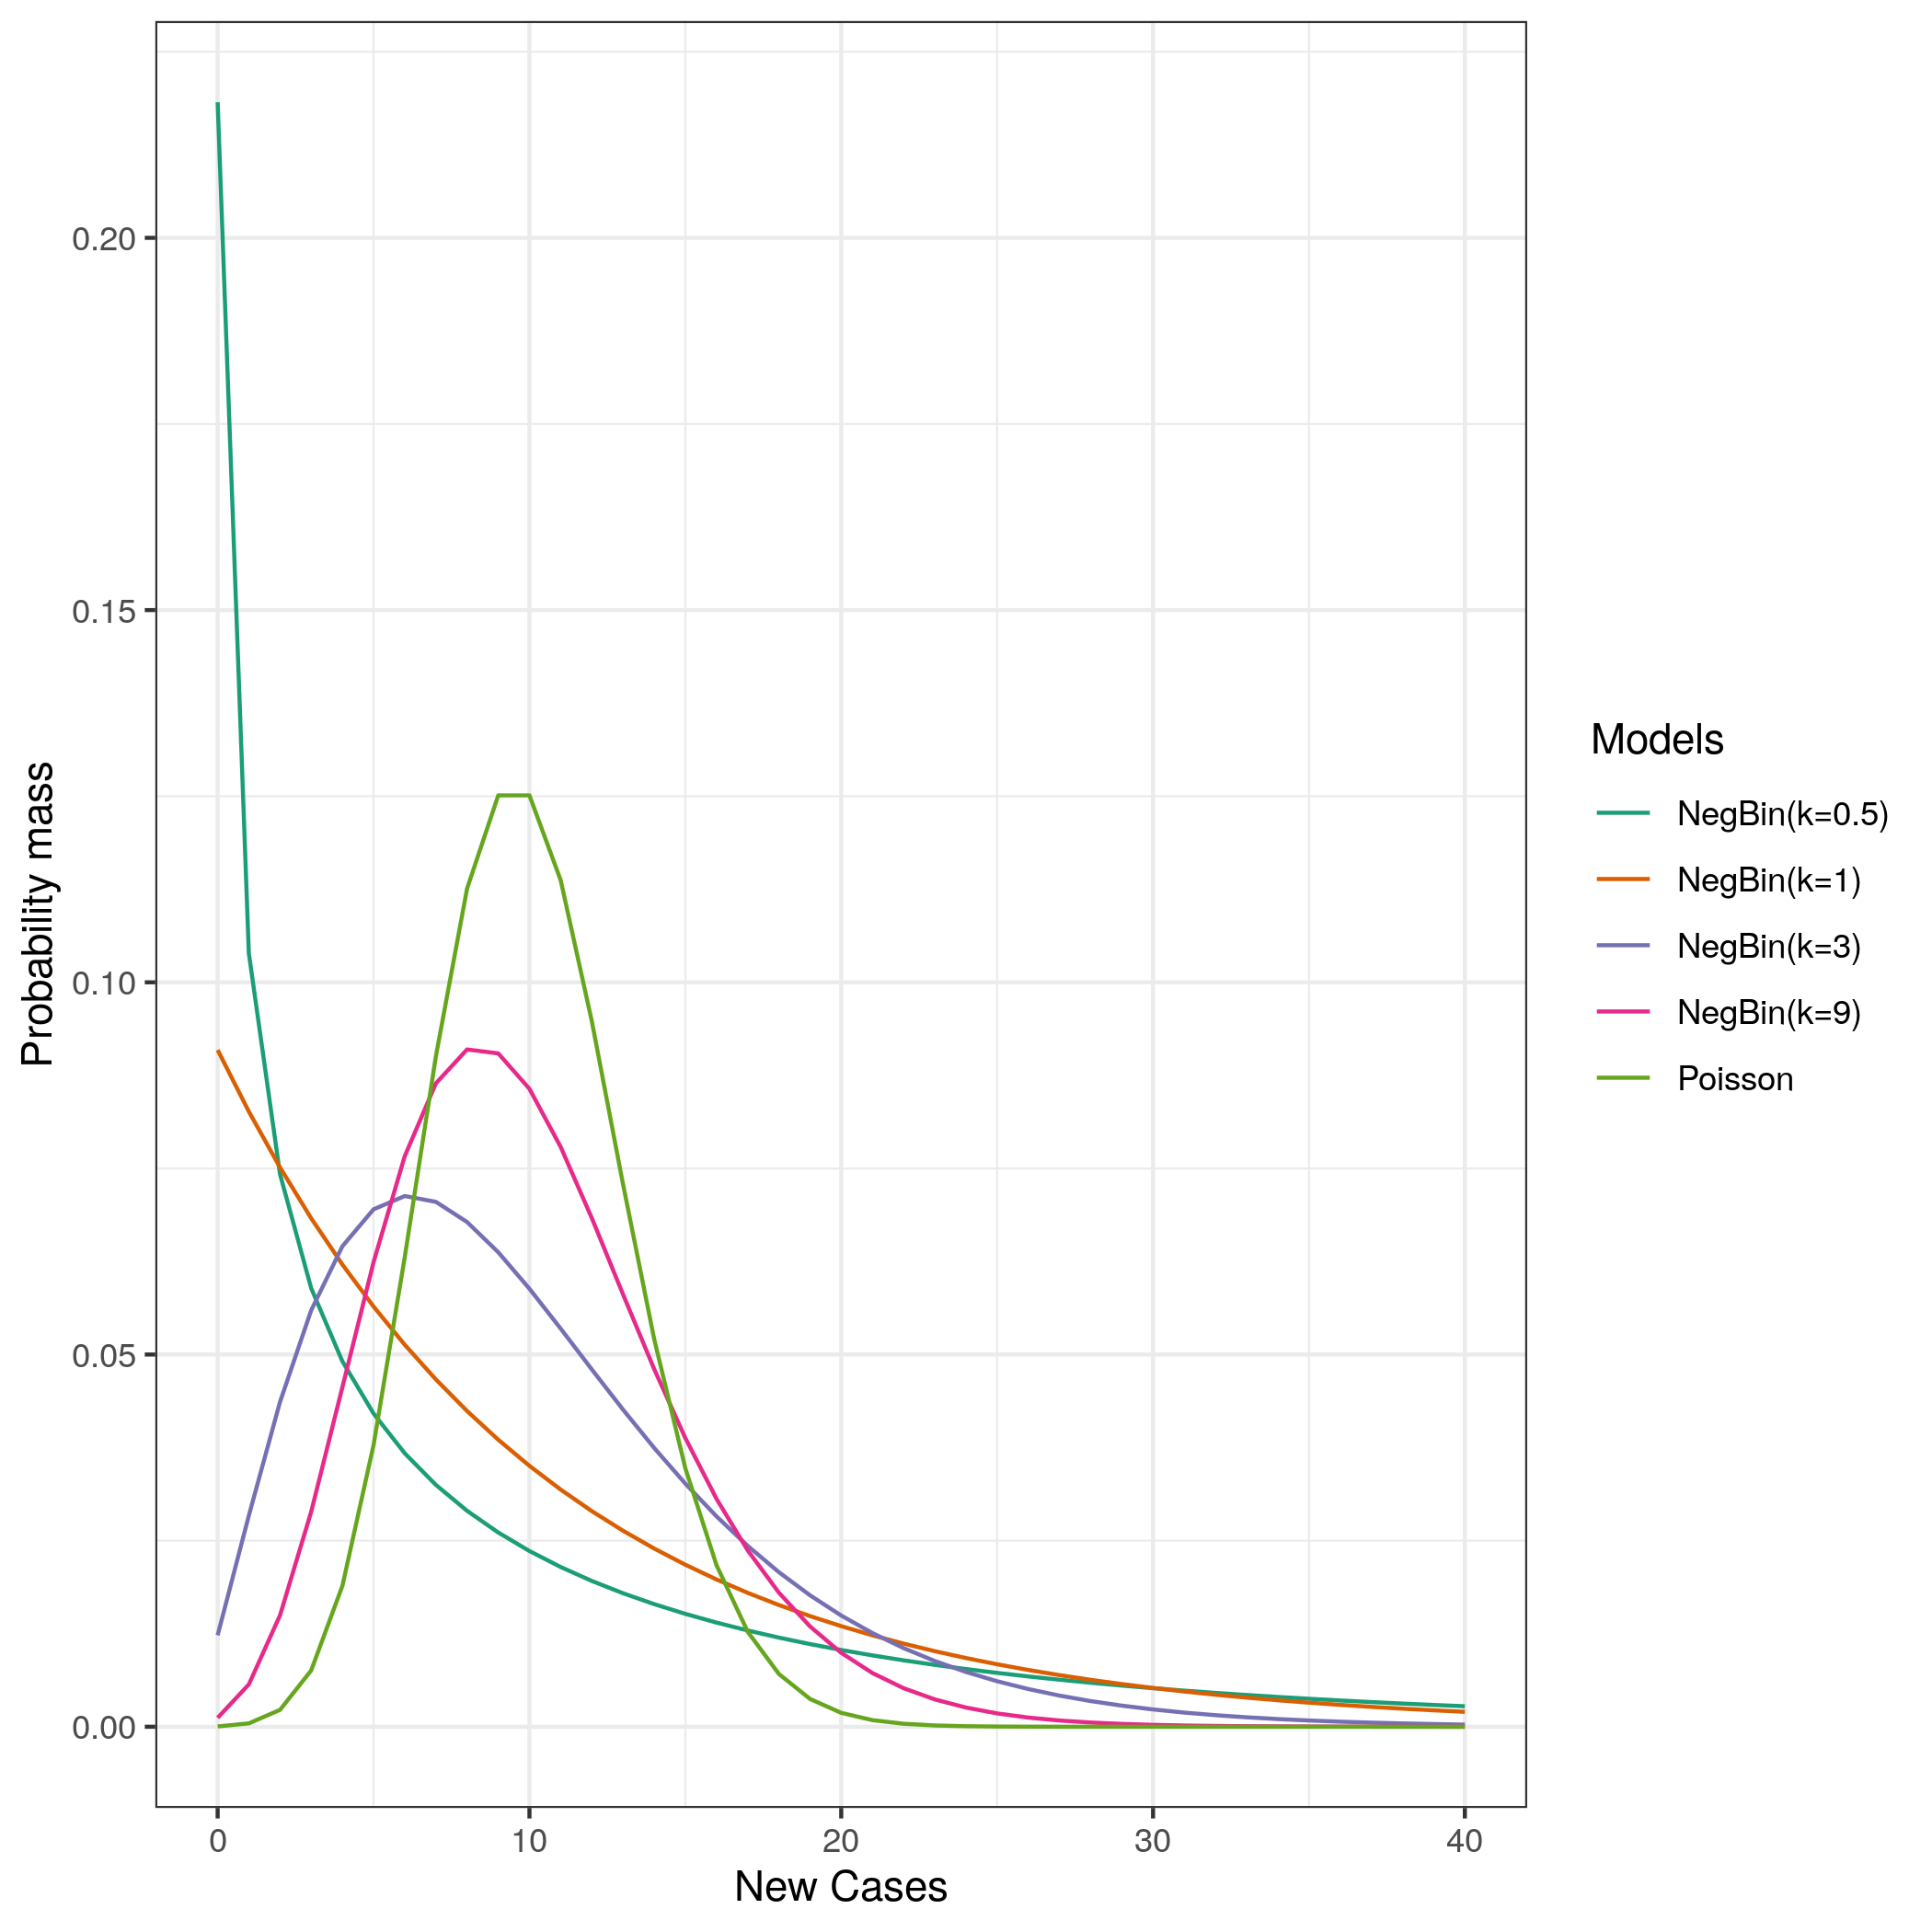
\includegraphics[width=\textwidth]{../output/tot_map.png}
  \caption{Total number of confirmed cases by health zone.}
  \label{fig:tot_map}
\end{subfigure}

\bigskip

\begin{subfigure}{\textwidth}
  \centering
  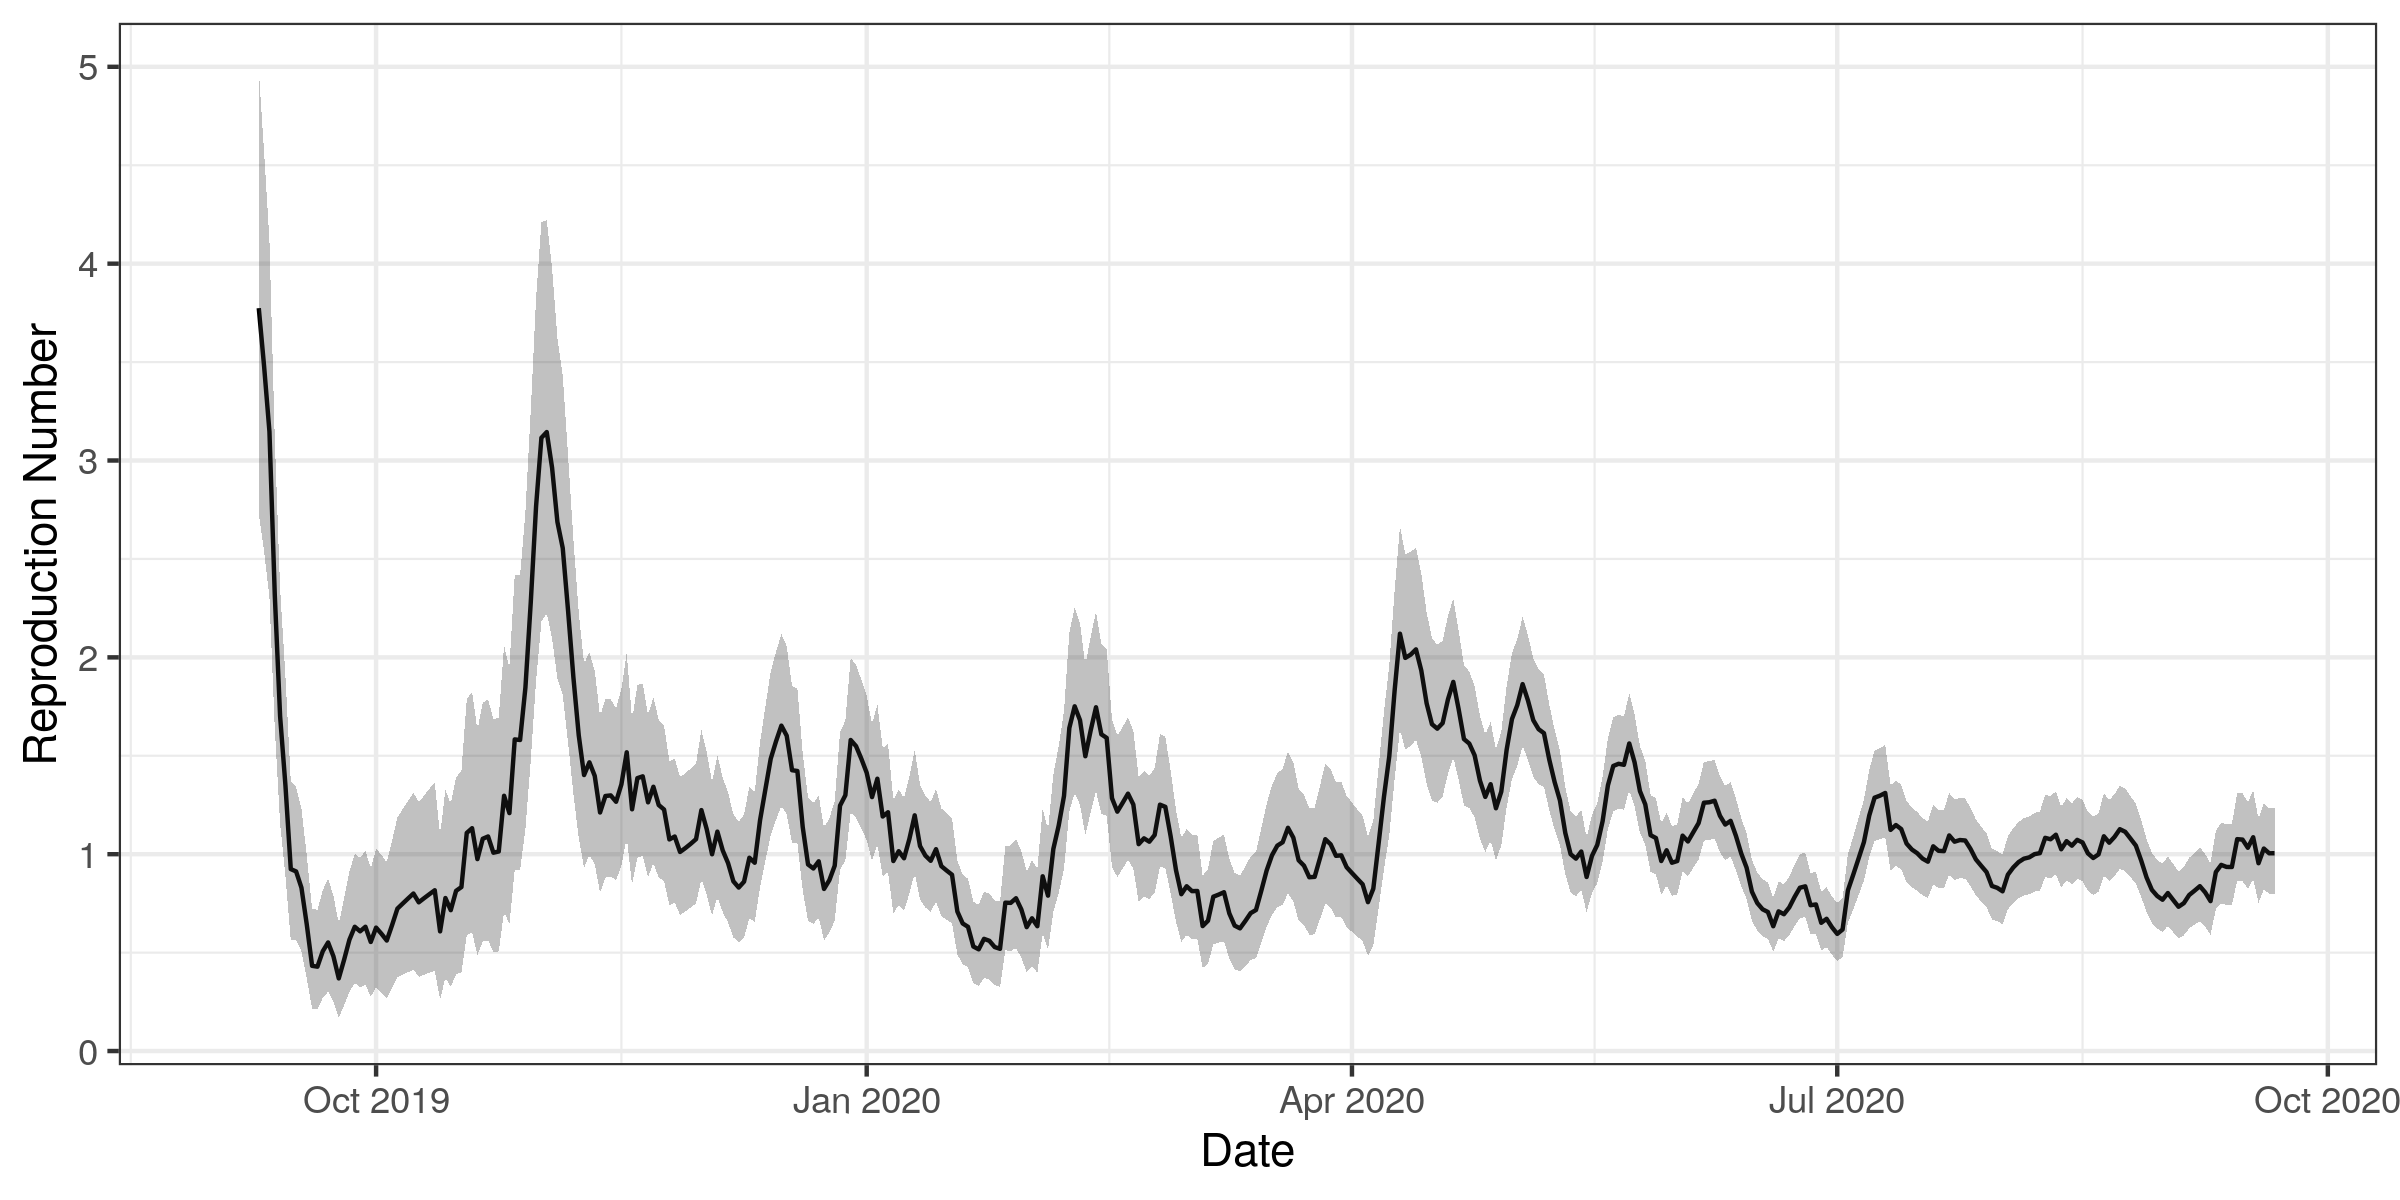
\includegraphics[width=\textwidth]{../output/nat_Rs.png}
  \caption{Mean estimated reproduction number as a function of time, with the shaded region showing the 95\% credible interval.}
  \label{fig:rep_num}
\end{subfigure}
\caption{The three figures show the number of cases and the reproduction number as a function of time and health zone.}
\label{fig:nat_outbreak}
\end{figure}

\subsection{National-level forecasts}
The first step in modelling the outbreak on the national level was to find the best fitting value of the dispersion parameter for the negative binomial models. We found that the dispersion parameter that gives the smallest RPS score for one-day-ahead predictions for the negative binomial models was $k\approx8$, but a fairly large range of parameters gave similar scores. We therefore chose to use $k=8$ for the negative binomial distributions both for the national and health zone forecasts.

All four of the models were fitted on incidence data from 395 days of national data and then used to provide short-term forecasts. The calibration and proper scoring rules scores for the four models for different forecasting horizons can be seen in Table \ref{tab:nat_evo} for weekly forecasting horizons up to four weeks. We also show the evolution of calibration, bias, RPS and the centrality of PIT values as a function of the forecasting horizon in Figure \ref{fig:national_scores}.
% latex table generated in R 3.6.1 by xtable 1.8-4 package
<<<<<<< HEAD
% Sat Sep  7 08:33:09 2019
=======
% Tue Sep 10 13:43:43 2019
>>>>>>> 6c96552641a3c339d41f2f58414064ece613e460
\begin{table}[ht]
\centering
\begin{tabular}{rlrrrrrrr}
  \hline
 & model & horizon & sharpness & bias & crps & dss & centrality & calibration \\ 
  \hline
<<<<<<< HEAD
1 & Negative Binomial Semilocal &   1 & 4.08 & -0.03 & 1.87 & 3.30 & 0.55 & 0.19 \\ 
  2 & Negative Binomial Latest &   1 & 4.14 & -0.00 & 1.82 & 3.26 & 0.56 & 0.17 \\ 
  3 & Poisson Semilocal &   1 & 2.93 & 0.01 & 1.87 & 3.32 & 0.43 & 0.00 \\ 
  4 & Poisson Latest &   1 & 2.97 & 0.05 & 1.82 & 3.24 & 0.42 & 0.00 \\ 
  5 & Negative Binomial Semilocal &   7 & 4.83 & -0.07 & 1.80 & 3.41 & 0.66 & 0.00 \\ 
  6 & Negative Binomial Latest &   7 & 4.33 & 0.01 & 2.36 & 3.94 & 0.47 & 0.00 \\ 
  7 & Poisson Semilocal &   7 & 4.19 & -0.02 & 1.72 & 3.23 & 0.59 & 0.01 \\ 
  8 & Poisson Latest &   7 & 3.08 & 0.06 & 2.47 & 4.31 & 0.36 & 0.00 \\ 
  9 & Negative Binomial Semilocal &  14 & 5.98 & -0.10 & 2.56 & 4.62 & 0.63 & 0.00 \\ 
  10 & Negative Binomial Latest &  14 & 4.62 & 0.02 & 2.82 & 4.74 & 0.41 & 0.00 \\ 
  11 & Poisson Semilocal &  14 & 5.78 & -0.06 & 2.52 & 4.54 & 0.60 & 0.00 \\ 
  12 & Poisson Latest &  14 & 3.28 & 0.09 & 2.99 & 5.32 & 0.29 & 0.00 \\ 
  13 & Negative Binomial Semilocal &  21 & 7.55 & -0.13 & 3.24 & 5.69 & 0.65 & 0.00 \\ 
  14 & Negative Binomial Latest &  21 & 5.12 & 0.01 & 4.07 & 5.57 & 0.31 & 0.00 \\ 
  15 & Poisson Semilocal &  21 & 7.67 & -0.10 & 3.26 & 5.88 & 0.65 & 0.00 \\ 
  16 & Poisson Latest &  21 & 3.53 & 0.06 & 4.54 & 6.85 & 0.24 & 0.00 \\ 
  17 & Negative Binomial Semilocal &  28 & 9.14 & -0.16 & 4.77 & 7.43 & 0.67 & 0.00 \\ 
  18 & Negative Binomial Latest &  28 & 5.87 & 0.03 & 5.30 & 7.38 & 0.30 & 0.00 \\ 
  19 & Poisson Semilocal &  28 & 9.64 & -0.13 & 4.89 & 7.12 & 0.66 & 0.00 \\ 
  20 & Poisson Latest &  28 & 3.88 & 0.08 & 6.00 & 9.08 & 0.22 & 0.00 \\ 
=======
1 & Negative Binomial Semilocal &   1 & 4.08 & -0.65 & 1.87 & 3.30 & 0.05 & 0.19 \\ 
  2 & Negative Binomial Latest &   1 & 4.14 & -0.65 & 1.82 & 3.26 & 0.06 & 0.16 \\ 
  3 & Poisson Semilocal &   1 & 2.93 & -0.65 & 1.87 & 3.32 & -0.07 & 0.00 \\ 
  4 & Poisson Latest &   1 & 2.97 & -0.65 & 1.82 & 3.24 & -0.08 & 0.00 \\ 
  5 & Negative Binomial Semilocal &   7 & 4.83 & -0.65 & 1.80 & 3.41 & 0.16 & 0.00 \\ 
  6 & Negative Binomial Latest &   7 & 4.33 & -0.65 & 2.36 & 3.94 & -0.04 & 0.00 \\ 
  7 & Poisson Semilocal &   7 & 4.19 & -0.65 & 1.72 & 3.23 & 0.09 & 0.01 \\ 
  8 & Poisson Latest &   7 & 3.08 & -0.65 & 2.47 & 4.31 & -0.14 & 0.00 \\ 
  9 & Negative Binomial Semilocal &  14 & 5.98 & -0.66 & 2.56 & 4.62 & 0.14 & 0.00 \\ 
  10 & Negative Binomial Latest &  14 & 4.62 & -0.66 & 2.82 & 4.74 & -0.08 & 0.00 \\ 
  11 & Poisson Semilocal &  14 & 5.78 & -0.66 & 2.52 & 4.54 & 0.10 & 0.00 \\ 
  12 & Poisson Latest &  14 & 3.28 & -0.66 & 2.99 & 5.32 & -0.21 & 0.00 \\ 
  13 & Negative Binomial Semilocal &  21 & 7.55 & -0.67 & 3.24 & 5.69 & 0.15 & 0.00 \\ 
  14 & Negative Binomial Latest &  21 & 5.12 & -0.67 & 4.07 & 5.57 & -0.19 & 0.00 \\ 
  15 & Poisson Semilocal &  21 & 7.67 & -0.67 & 3.26 & 5.88 & 0.16 & 0.00 \\ 
  16 & Poisson Latest &  21 & 3.53 & -0.67 & 4.54 & 6.85 & -0.26 & 0.00 \\ 
  17 & Negative Binomial Semilocal &  28 & 9.14 & -0.68 & 4.77 & 7.43 & 0.17 & 0.00 \\ 
  18 & Negative Binomial Latest &  28 & 5.87 & -0.68 & 5.30 & 7.38 & -0.20 & 0.00 \\ 
  19 & Poisson Semilocal &  28 & 9.64 & -0.68 & 4.89 & 7.12 & 0.16 & 0.00 \\ 
  20 & Poisson Latest &  28 & 3.88 & -0.68 & 6.00 & 9.08 & -0.28 & 0.00 \\ 
>>>>>>> 6c96552641a3c339d41f2f58414064ece613e460
   \hline
\end{tabular}
\caption{Model evaluations for predictions when all the models are fitted on the combined data from all the health zones.} 
\label{tab:nat_evo}
\end{table}



\begin{figure}[h!]
\begin{subfigure}{0.5\textwidth}
  \centering
  % include first image
  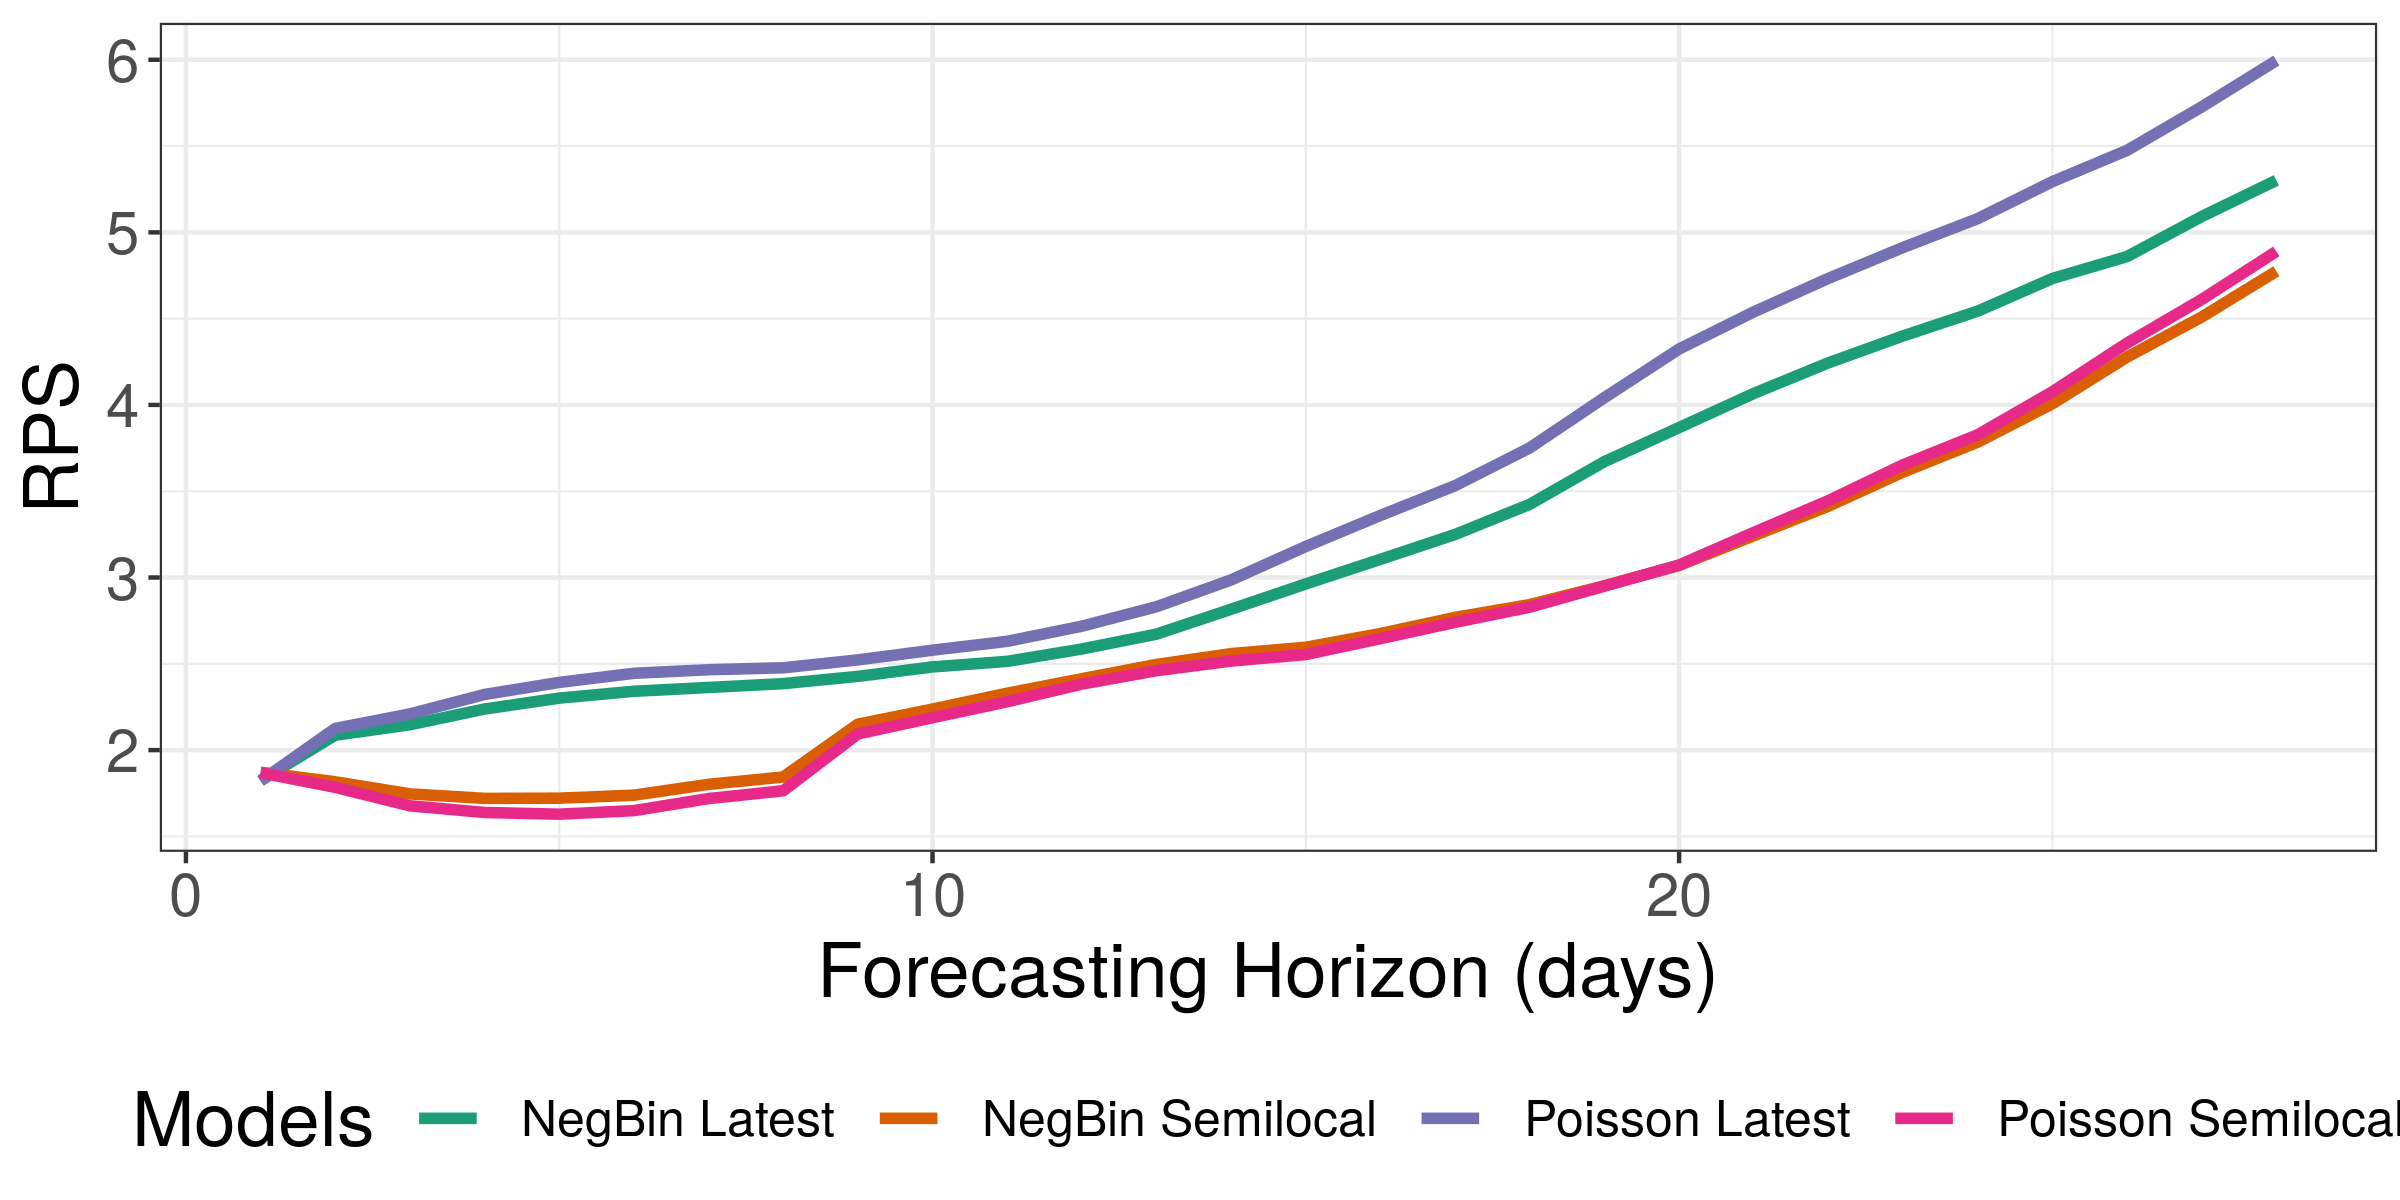
\includegraphics[width=\linewidth]{../output/national_crps.png}  
  \caption{Ranked Probability Score}
  \label{fig:sub-first}
\end{subfigure}
\begin{subfigure}{0.5\textwidth}
  \centering
  % include second image
  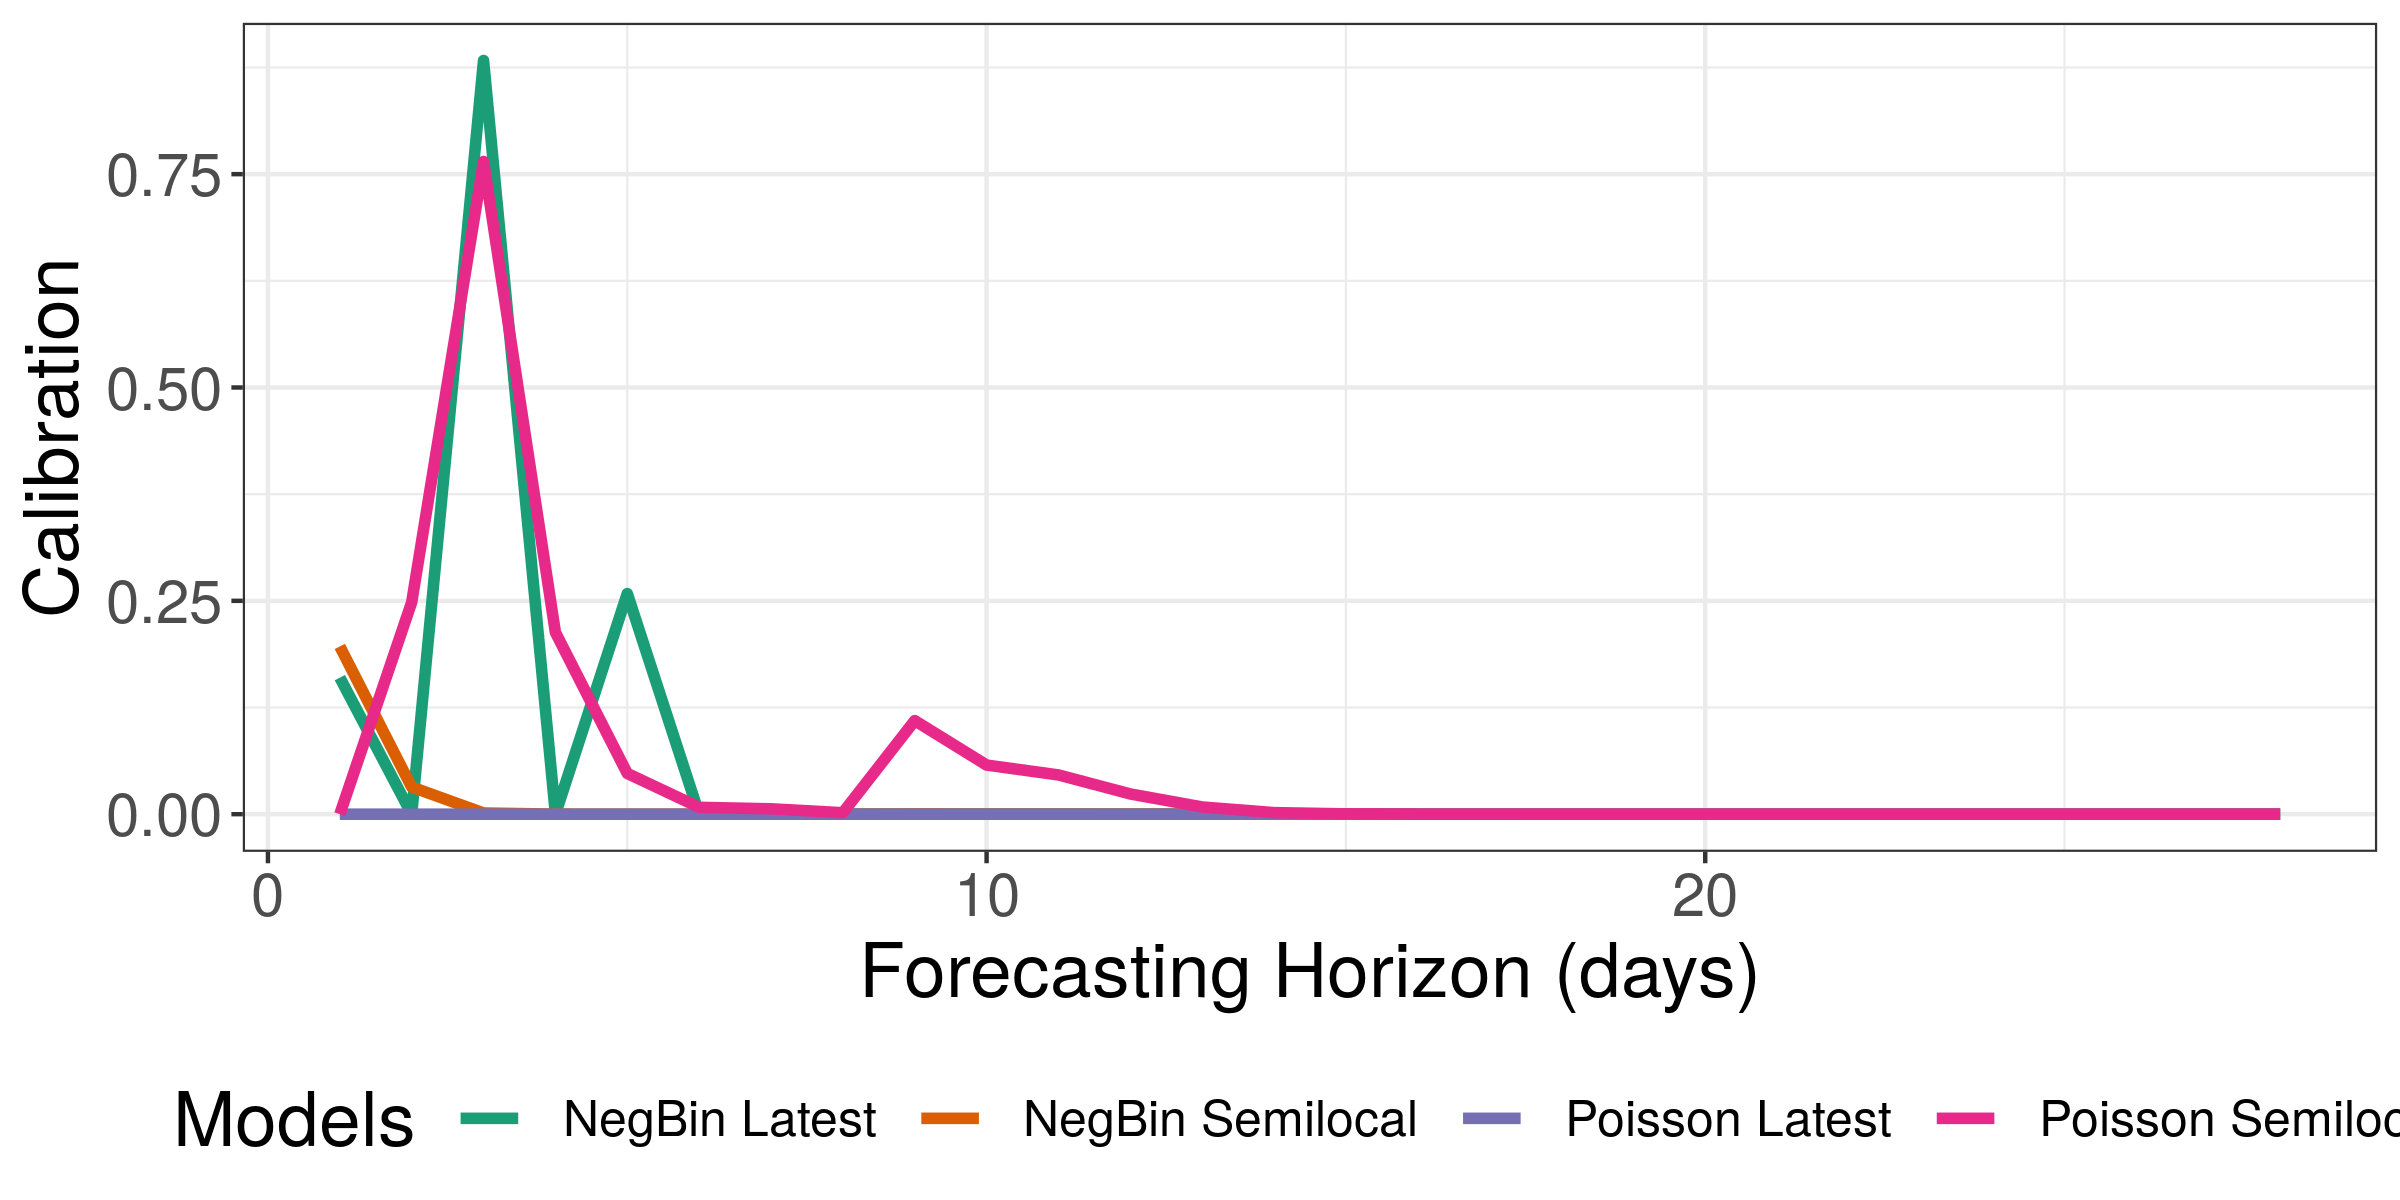
\includegraphics[width=\linewidth]{../output/national_calibration.png}  
  \caption{P-value for calibration of PIT values}
  \label{fig:sub-second}
\end{subfigure}

\begin{subfigure}{0.5\textwidth}
  \centering
  % include second image
  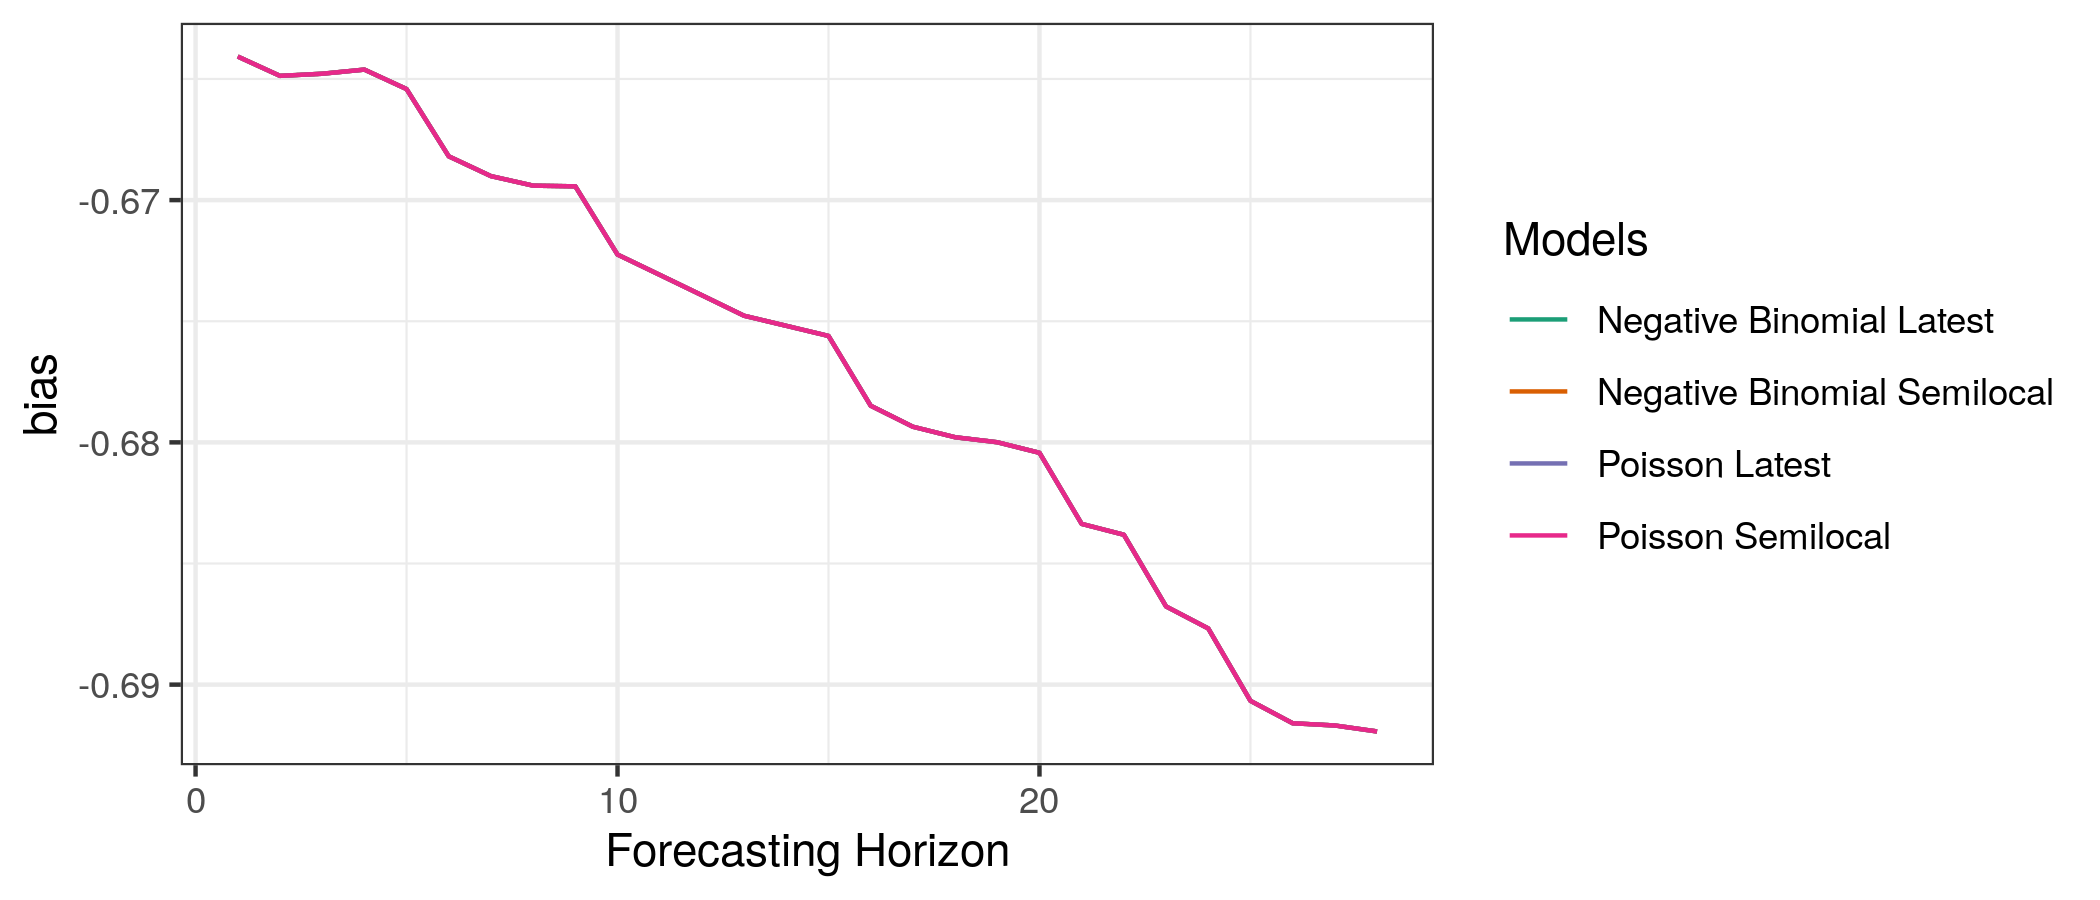
\includegraphics[width=\linewidth]{../output/national_bias.png}  
  \caption{Bias}
  \label{fig:sub-third}
\end{subfigure}
\begin{subfigure}{0.5\textwidth}
  \centering
  % include second image
  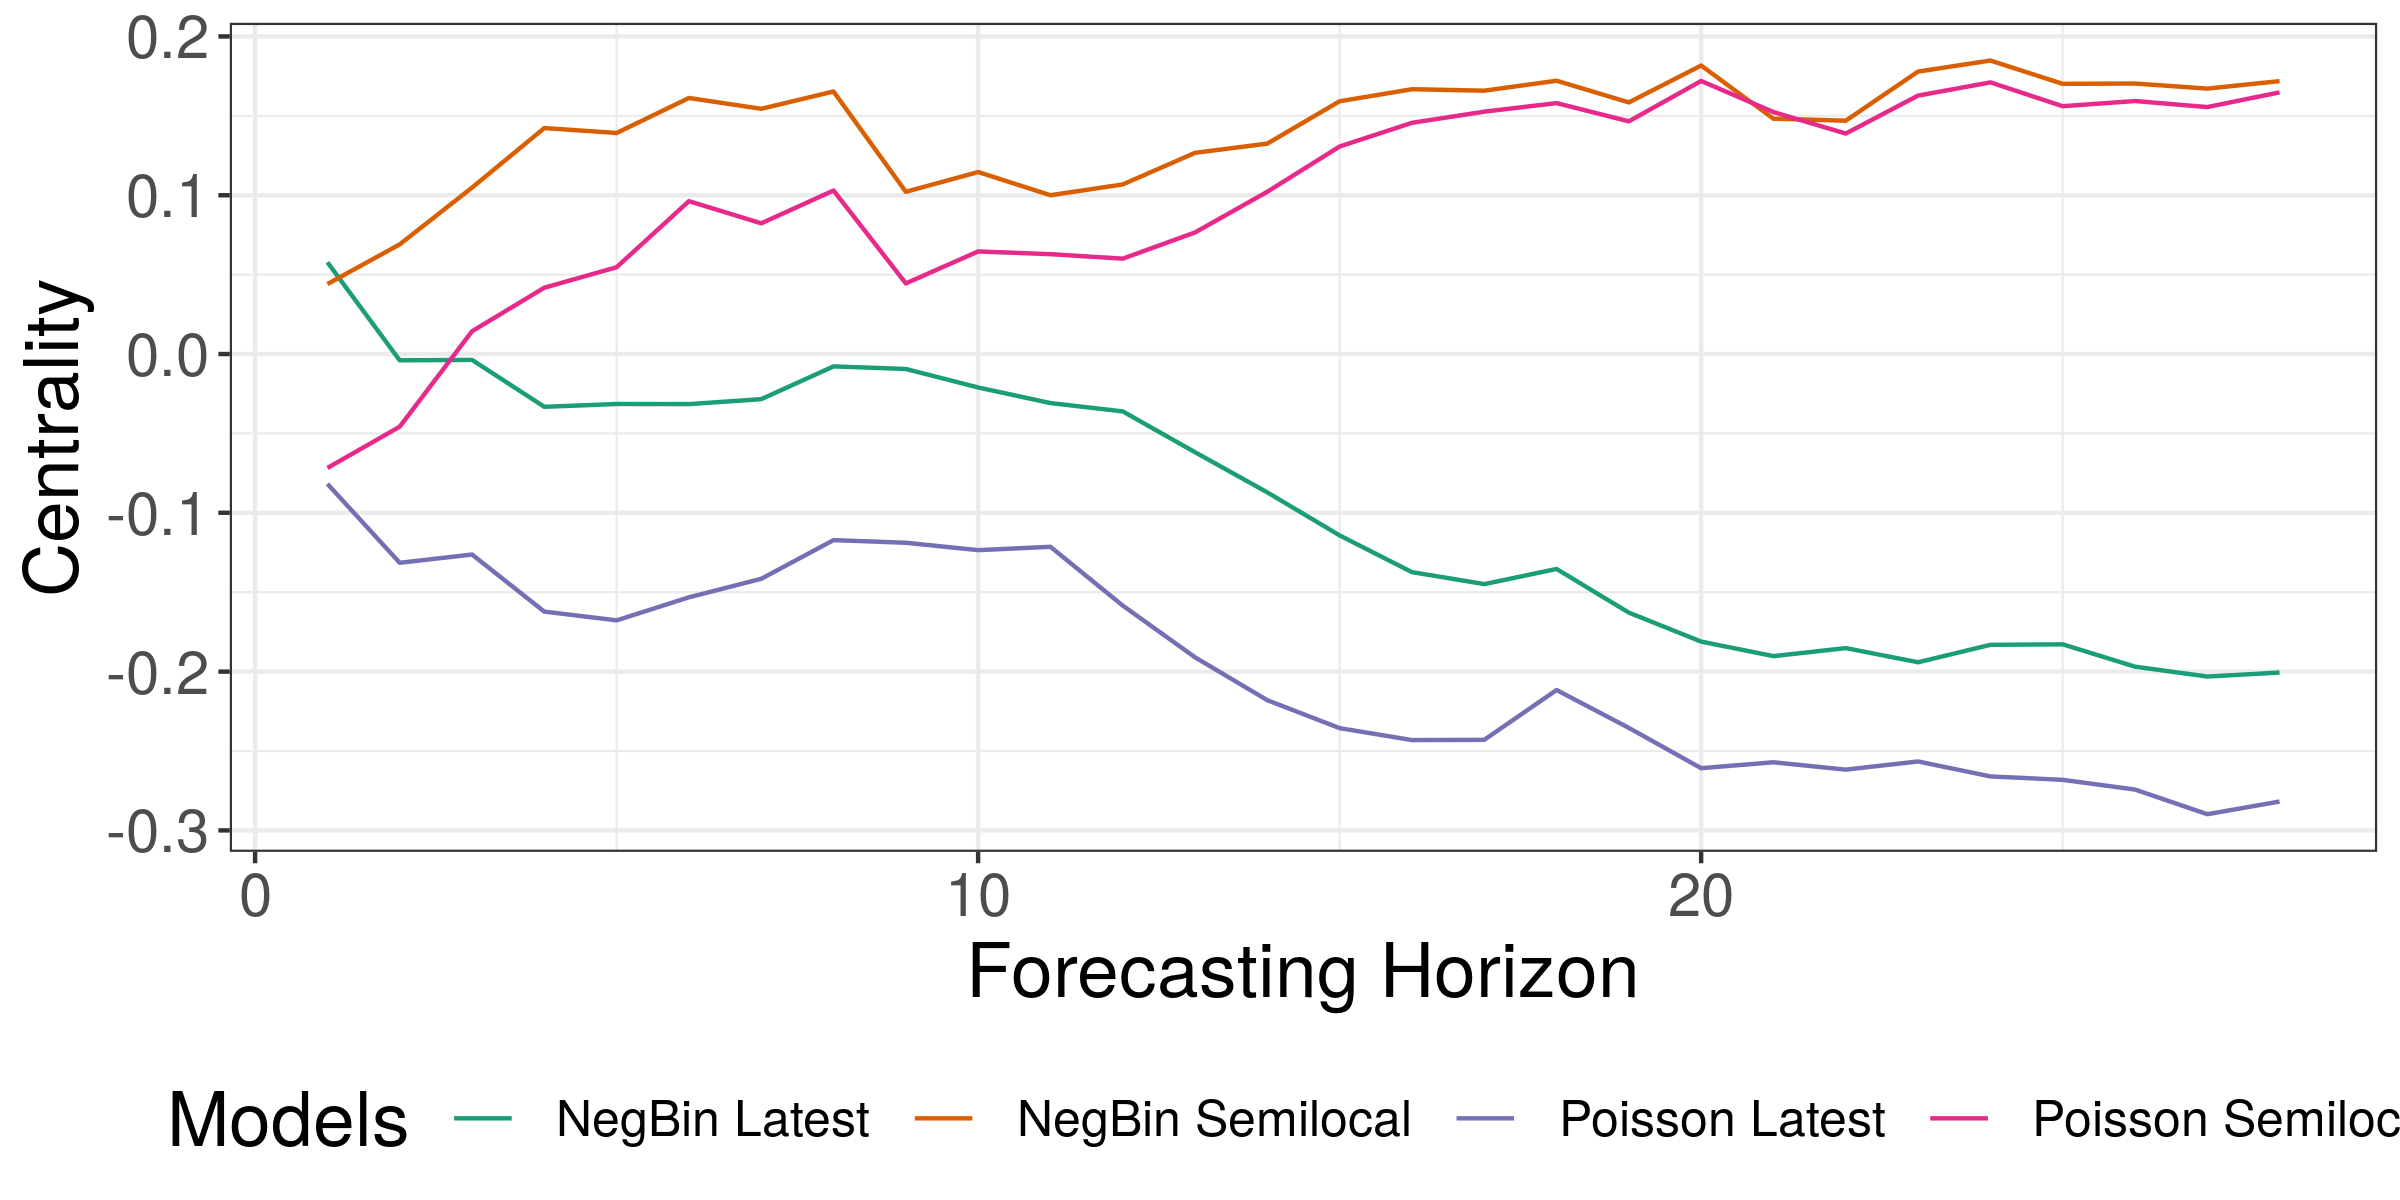
\includegraphics[width=\linewidth]{../output/national_centrality.png}  
  \caption{Centrality of PIT values}
  \label{fig:nat_scores_4}
\end{subfigure}
  \caption{Evaluation of the four models as a function of forecasting horizon at the national level.}

  \label{fig:national_scores}
\end{figure}

Together they show that for next-day forecasts, the negative binomial offspring distribution is needed for a calibrated forecast as only the two negative binomial models are calibrated with a p-value larger than 0.1. We can also see that there are no big differences for one-day-ahead forecasts based on the method of forecasting the reproduction number. For longer forecasting horizons, the Poisson distribution with the semi-local time series prediction for $R_t$ is the best model and is calibrated up until a maximum of nine days even if it is not well calibrated for all the days before. This is the only model that is calibrated for longer forecasting horizons and it also has the lowest RPS and DSS scores. The Poisson model with a constant reproduction number could not provide any calibrated forecasts, the negative binomial model with a constant reproduction number was calibrated during the first 5 days, and the negative binomial model with a semi-local trend in the reproduction number was only calibrated for the first day.

The centrality of the PIT scores in Figure \ref{fig:nat_scores_4} gives us extra information about why the models become uncalibrated. A negative centrality means that the model has too little uncertainty, and we can see that this is the case for the two models based on using the latest reproduction number. The two models using the semi-local trend for the reproduction number are closer to zero centrality, but they have too much uncertainty since their centrality score is above zero. For the same method of forecasting the reproduction number, the negative binomial models always have a larger uncertainty, as we can also see from the sharpness figures. This is why the Poisson model is preferred at larger forecasting horizons. After about one week, the sharpness of the Poisson semi-local model has grown to be the same as the negative binomial model with a constant reproduction number. We can see how the semi-local models quickly become less sharp, while the sharpness of the constant models does not change as much with the forecasting horizon. The two semi-local models have a small negative bias indicating that on average they underestimate the incidence.

In Figure \ref{fig:nat_pred} we show 28-day forecasts every 50 days for the semi-local Poisson model and the corresponding forecasts for the reproduction number. These results show the same pattern as the more formal evaluations. In the short term the model works quite well, but the amount of uncertainty often seems a bit too large for the reproduction number forecasts. We also forecast the incidence for the 28 days following the 1st of September 2019 in Figure \ref{fig:nat_pred}. Here the model predicts a slightly decreasing median reproduction number and a fairly steady incidence through the month of September. We expect between 10--15 cases per day over the next month. 

\begin{figure}[h!]
\begin{subfigure}{\textwidth}
  \centering
  % include first image
  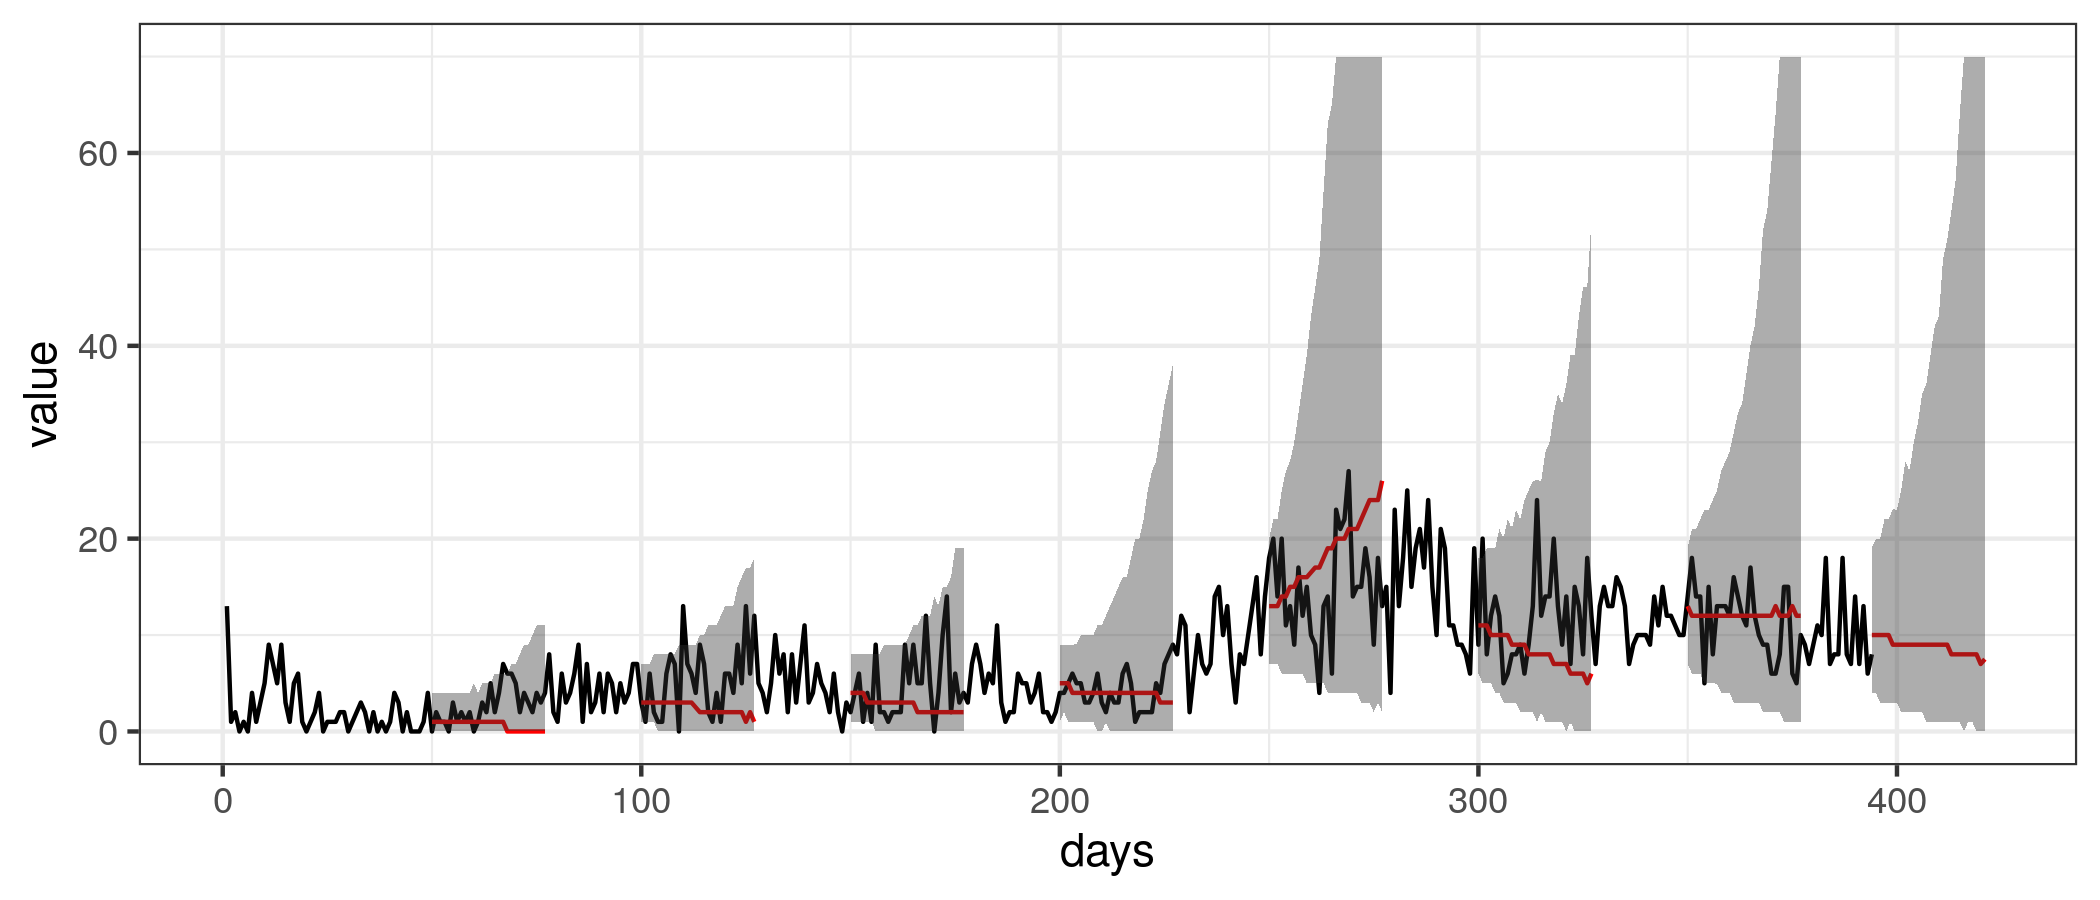
\includegraphics[width=0.9\linewidth, height=7cm]{../output/national_predictions.png}  
  \caption{Forecasted and predicted incidence for the semi-local Poisson model}
  \label{fig:sub-first}
\end{subfigure}

\begin{subfigure}{\textwidth}
  \centering
  % include second image
  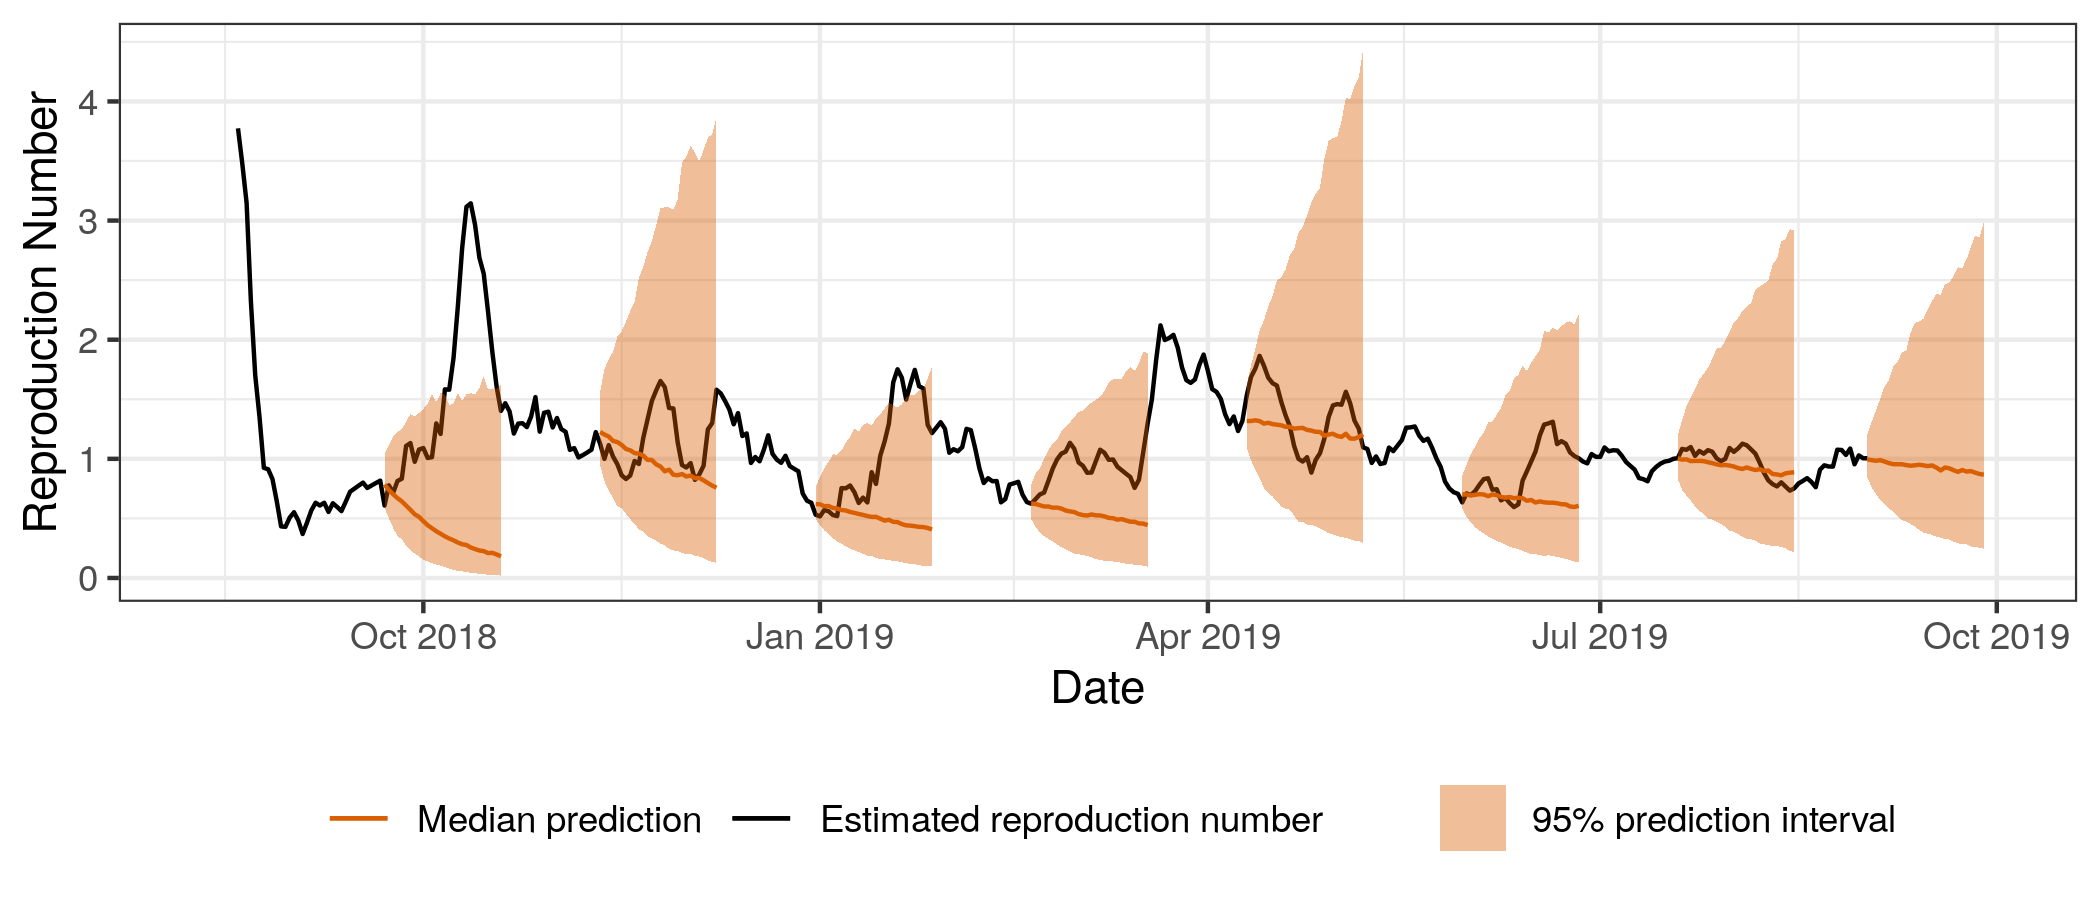
\includegraphics[width=0.9\linewidth, height=7cm]{../output/national_Rs.png}  
  \caption{Forecasted and predicted reproduction numbers for the semi-local Poisson model}
  \label{fig:sub-second}
\end{subfigure}
  \caption{Median forecast with 95\% prediction intervals and observed values for incidence and reproduction number for the semi-local Poisson model.}

  \label{fig:nat_pred}
\end{figure}

\subsection{Sub-national forecasts}

We fitted all four models separately for each health zone that had more than one case of Ebola. The performance of the models varied significantly from health zone to health zone. Table \ref{tab:best_model} shows the best model(s) for each health zone, how large a forecasting horizon we can have without ruling out calibration, and the total number of confirmed cases in the health zone. There is a large difference ranging from health zones where the forecasts are calibrated for 28 days to health zones where not even the one-day-ahead predictions are calibrated. Even if the model is calibrated at 28 days, it does not mean that it is calibrated for all forecasting horizons less than 28 days. 


% latex table generated in R 3.6.1 by xtable 1.8-4 package
% Tue Sep 24 17:36:32 2019
\begin{table}[h!]
\centering
\begin{tabular}{|l|l|l|l|}
  \hline
Location & Largest Horizon & Best model & Cases \\ 
  \hline
Kayna & 28 & NegBin Semilocal & 22 \\ 
  Nyiragongo & 28 & NegBin Semilocal & 3 \\ 
  Tchomia & 28 & NegBin Semilocal & 2 \\ 
  Lolwa & 26 & All models & 3 \\ 
  Mwenga & 18 & All models & 6 \\ 
  Bunia & 17 & NegBin Semilocal & 4 \\ 
  Alimbongo & 12 & NegBin Semilocal & 5 \\ 
  national & 9 & Poisson Semilocal & 2942 \\ 
  Kayina & 7 & Poisson Semilocal & 10 \\ 
  Rwampara & 6 & NegBin Latest & 8 \\ 
  Lubero & 4 & NegBin Semilocal & 31 \\ 
  Musienene & 4 & Poisson Semilocal & 84 \\ 
  Kyondo & 3 & Poisson Semilocal & 22 \\ 
  Vuhovi & 3 & Poisson Semilocal & 103 \\ 
  Beni & 2 & Poisson Semilocal & 661 \\ 
  Biena & 2 & Poisson Latest & 16 \\ 
  Butembo & 2 & NegBin Semilocal & 279 \\ 
  Mabalako & 2 & NegBin Semilocal & 371 \\ 
  Kalunguta & NA & No calibrated model & 164 \\ 
  Katwa & NA & No calibrated model & 647 \\ 
  Mangurujipa & NA & No calibrated model & 20 \\ 
  Masereka & NA & No calibrated model & 50 \\ 
  Mutwanga & NA & No calibrated model & 31 \\ 
  Oicha & NA & No calibrated model & 55 \\ 
  Komanda & NA & No calibrated model & 43 \\ 
  Mambasa & NA & No calibrated model & 32 \\ 
  Mandima & NA & No calibrated model & 264 \\ 
   \hline
\end{tabular}
\caption{For each health zone we show the maximal forecasting horizon where we can not exclude calibration at the p=0.1 level. If multiple models are equally calibrated we chosse the one with smallest RPS. For some health zones there were no calibrated forecasts} 
\label{tab:best_model}
\end{table}


For all health zones apart from two, we find that the best model is a model with a semi-local trend in the reproduction number. Sometimes the Poisson models are better and sometimes the negative binomial models are better. The health zones where we get very well calibrated models at 28 days are health zones with small bursts of Ebola activity followed by long periods of no cases. Tchomia health zone is a good example of this and the forecasts can be seen in the Appendix. The models provide calibrated forecasts for some of the larger health zones where there is more sustained transmission, but not as well as on the national level. There are also some health zones with a large number of cases where the models do not work well. We show the predictions and the centrality measures for the Beni and Katwa health zones in Figure \ref{fig:beni_katwa}. The forecasts and evaluations for a selected number of other health zones can be seen in the Appendix. For both Beni and Katwa, the main reason the models are not well calibrated is that they overestimated their own uncertainty. This is especially the case in Katwa and explains why even the one-day-ahead prediction is not well calibrated. 

\begin{figure}[h!]
\begin{subfigure}{0.5\textwidth}
  \centering
  % include first image
  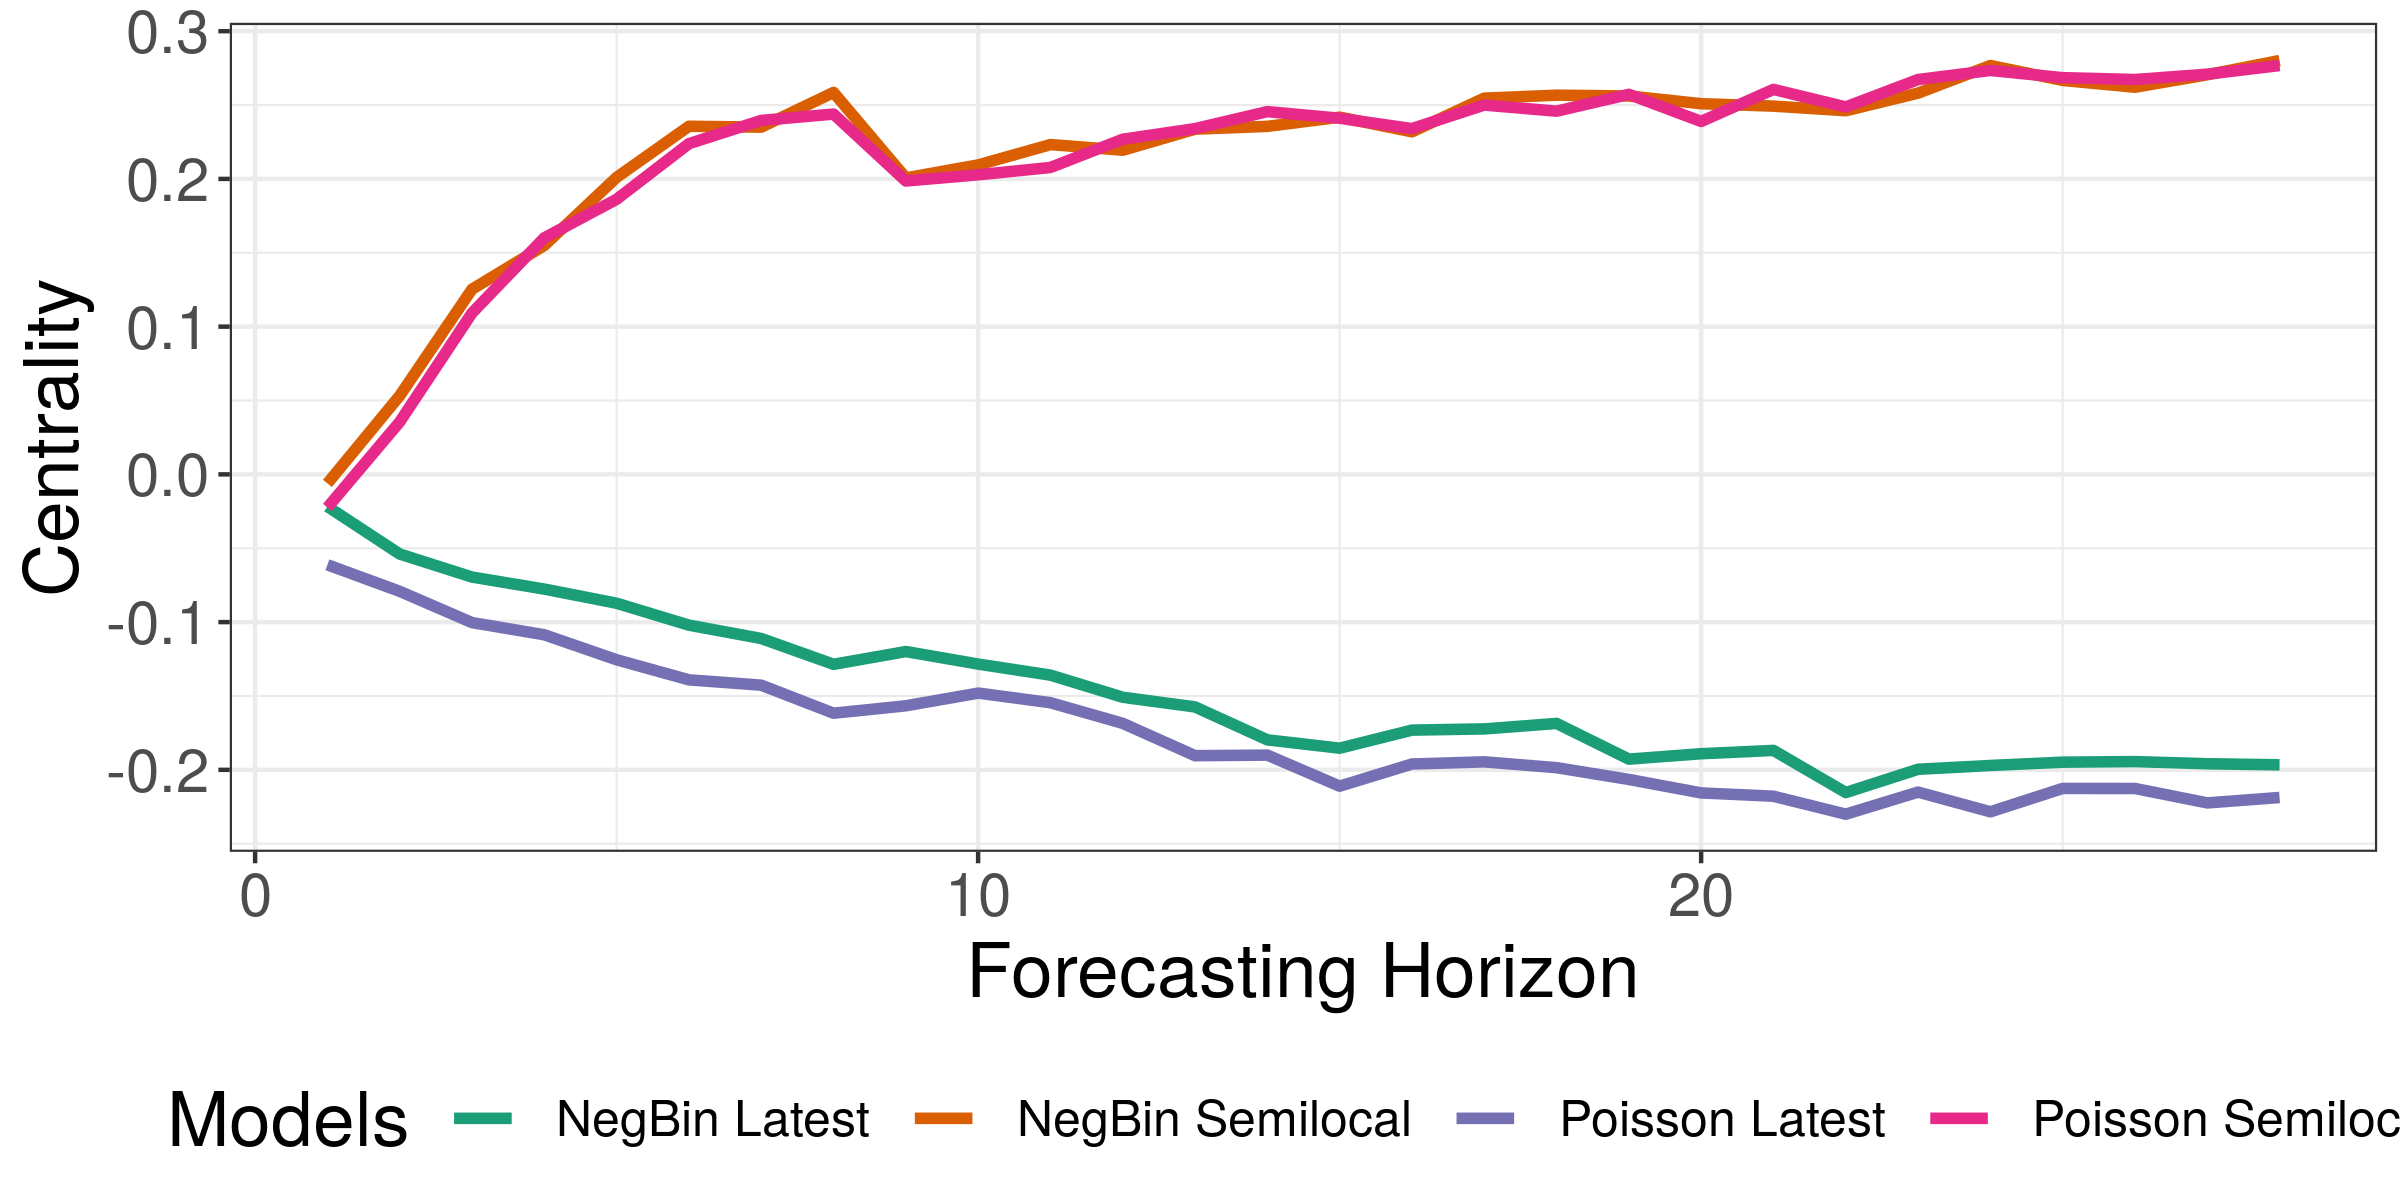
\includegraphics[width=\linewidth, ]{../output/Katwa_centrality.png}  
  \caption{Centrality of PIT values for the models in Katwa health zone }
  \label{fig:beni_katwa_1}
\end{subfigure}
\begin{subfigure}{0.5\textwidth}
  \centering
  % include second image
  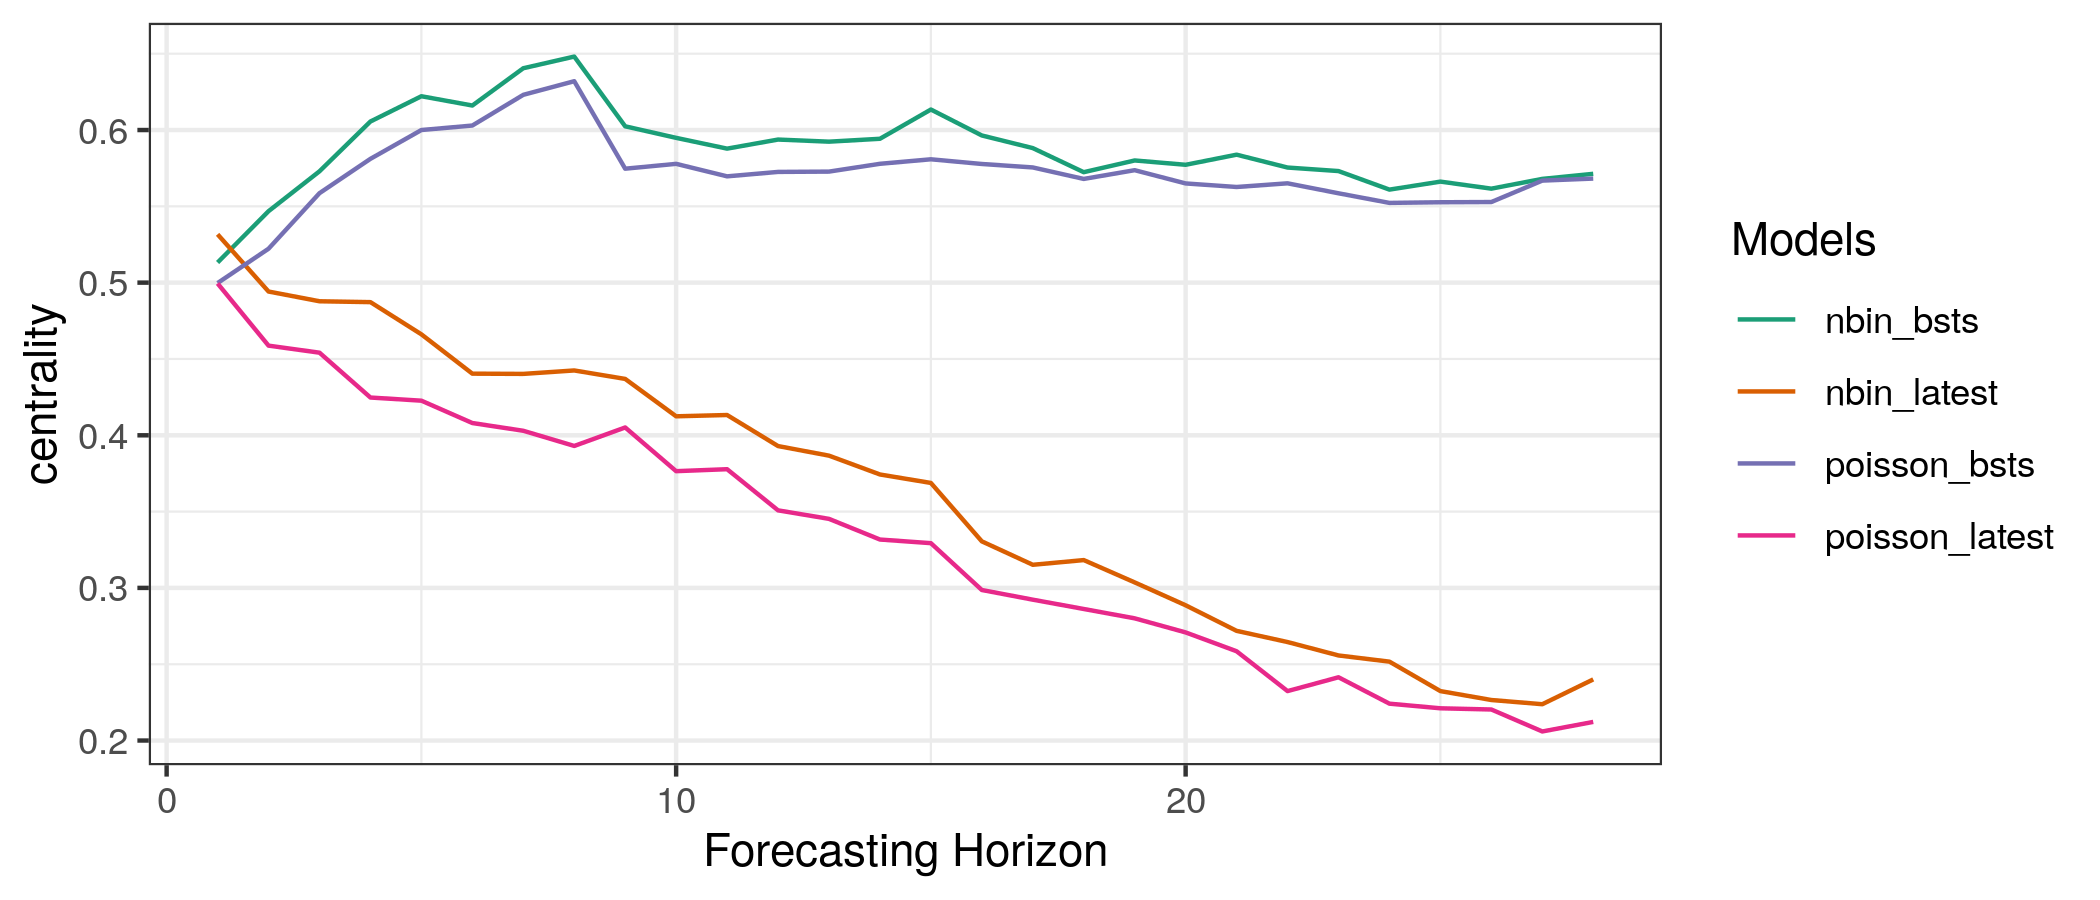
\includegraphics[width=\linewidth]{../output/Beni_centrality.png}  
  \caption{Centrality of PIT values for the models in Beni health zone}
  \label{fig:beni_katwa_2}
\end{subfigure}

\begin{subfigure}{\textwidth}
  \centering
  % include first image
  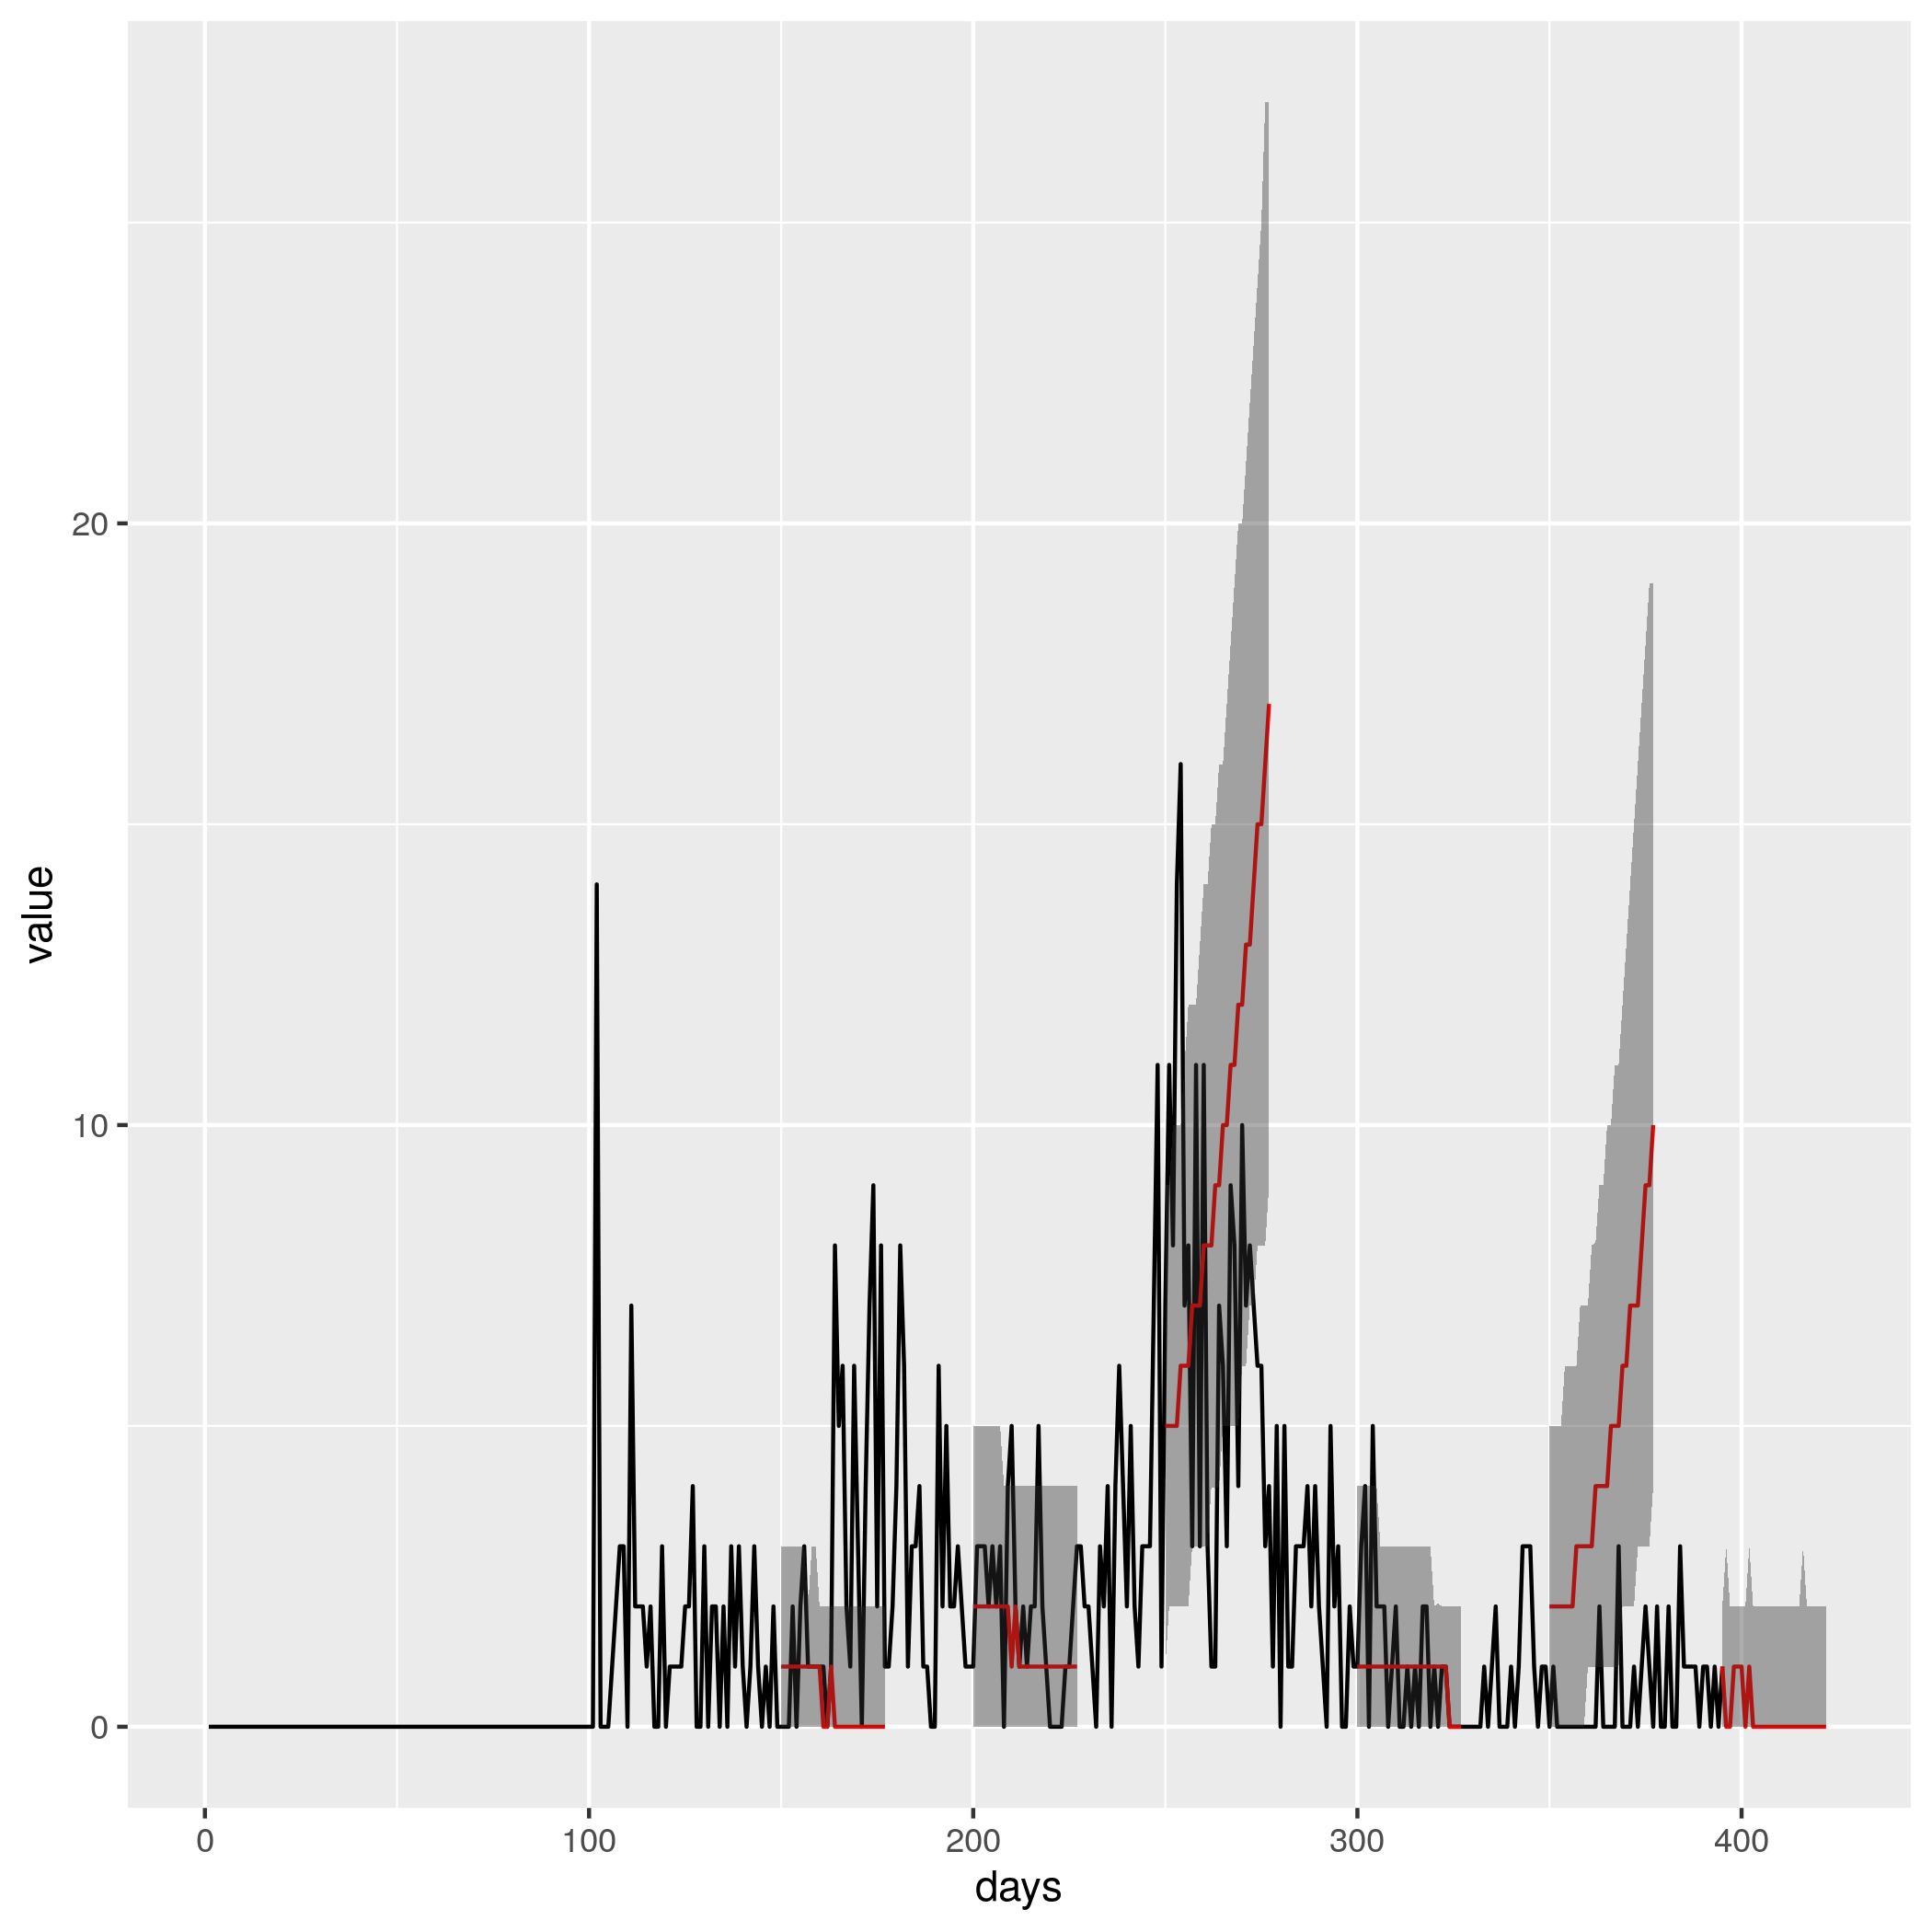
\includegraphics[width=0.9\linewidth, height=6.6cm]{../output/Katwa_predictions.png}  
  \caption{ Median forecast with 95\% prediction intervals and observed values for incidence for the Poisson semi-local model in Katwa}
  \label{fig:beni_katwa_3}
\end{subfigure}

\begin{subfigure}{\textwidth} 
  \centering
  % include second image
  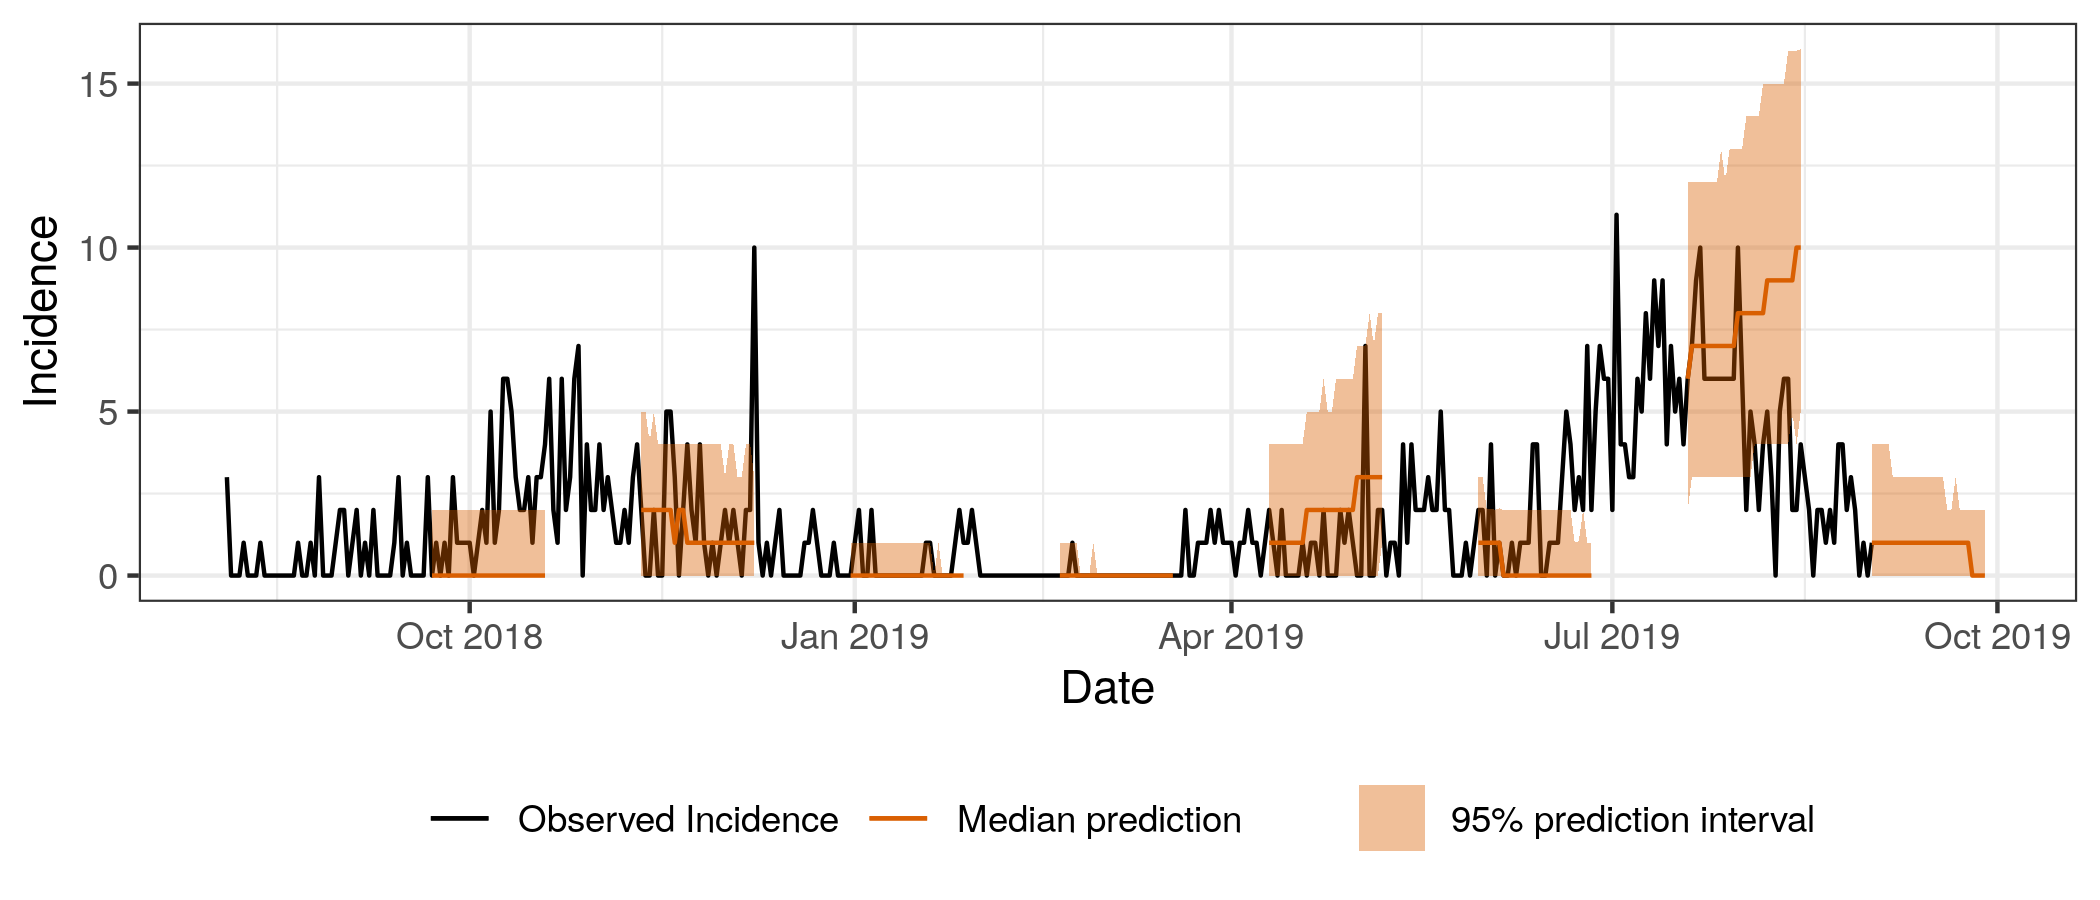
\includegraphics[width=0.9\linewidth, height=6.6cm]{../output/Beni_predictions.png}
  \caption{ Median forecast with 95\% prediction intervals and observed values for incidence for the Poisson semi-local model in Beni}
  \label{fig:beni_katwa_4}
\end{subfigure}
\caption{Evaluations and prediction for Katwa and Beni.}


\label{fig:beni_katwa}
\end{figure}

We used two methods to assess if the health zone model overall provided good forecasts. The first method was to combine the scores and PIT values, and we found that this gave clear evidence that the overall health zone model was uncalibrated at all forecasting horizons with p-values less than 0.001. The Ranked Probability Score and centrality from this combination of the scores in Figure \ref{fig:combined_hz_scores} shows that on the combined level the models with semi-local trend produce significantly better forecasts, but overestimate the uncertainty as they did on the national level. The combined bias also showed a positive bias indicating that on average the models forecast too large incidence. 

\begin{figure}[h!]
\begin{subfigure}{0.5\textwidth}
  \centering
  % include first image
  \includegraphics[width=\linewidth]{../output/hz_combined_crps.png}  
  \caption{Ranked Probability Score}
  \label{fig:sub-first}
\end{subfigure}
\begin{subfigure}{0.5\textwidth}
  \centering
  % include second image
  \includegraphics[width=\linewidth]{../output/hz_combined_centrality.png}  
  \caption{Centrality of the Randomised Probability Transform histogram}
  \label{fig:sub-second}
\end{subfigure}

  \caption{Ranked Probability Scores and centrality scores for the combined health-zone-level forecasts. RPS calculated as an average of scores from individual health zones and the centrality by combining all the randomised PIT values into one historgram.}

  \label{fig:combined_hz_scores}
\end{figure}



The second method to check the overall performance of the health zone model was by aggregating the forecasts from each health zone and comparing that to the national forecast model. Figure \ref{fig:nat_nat_comb} shows the comparison of the one-day-ahead predictions of the national-level model with the one-day-ahead predictions obtained by aggregating over all health zones when we used the semi-local Poisson model for all the locations. The predictions are fairly close, but when looking at the  calibration we find that the combined model is not calibrated and is also biased to predict too large incidence. The centrality scores for the combined models show that it actually underestimates the uncertainty at large forecasting horizons. 

\begin{figure}[h!]
  \centering
  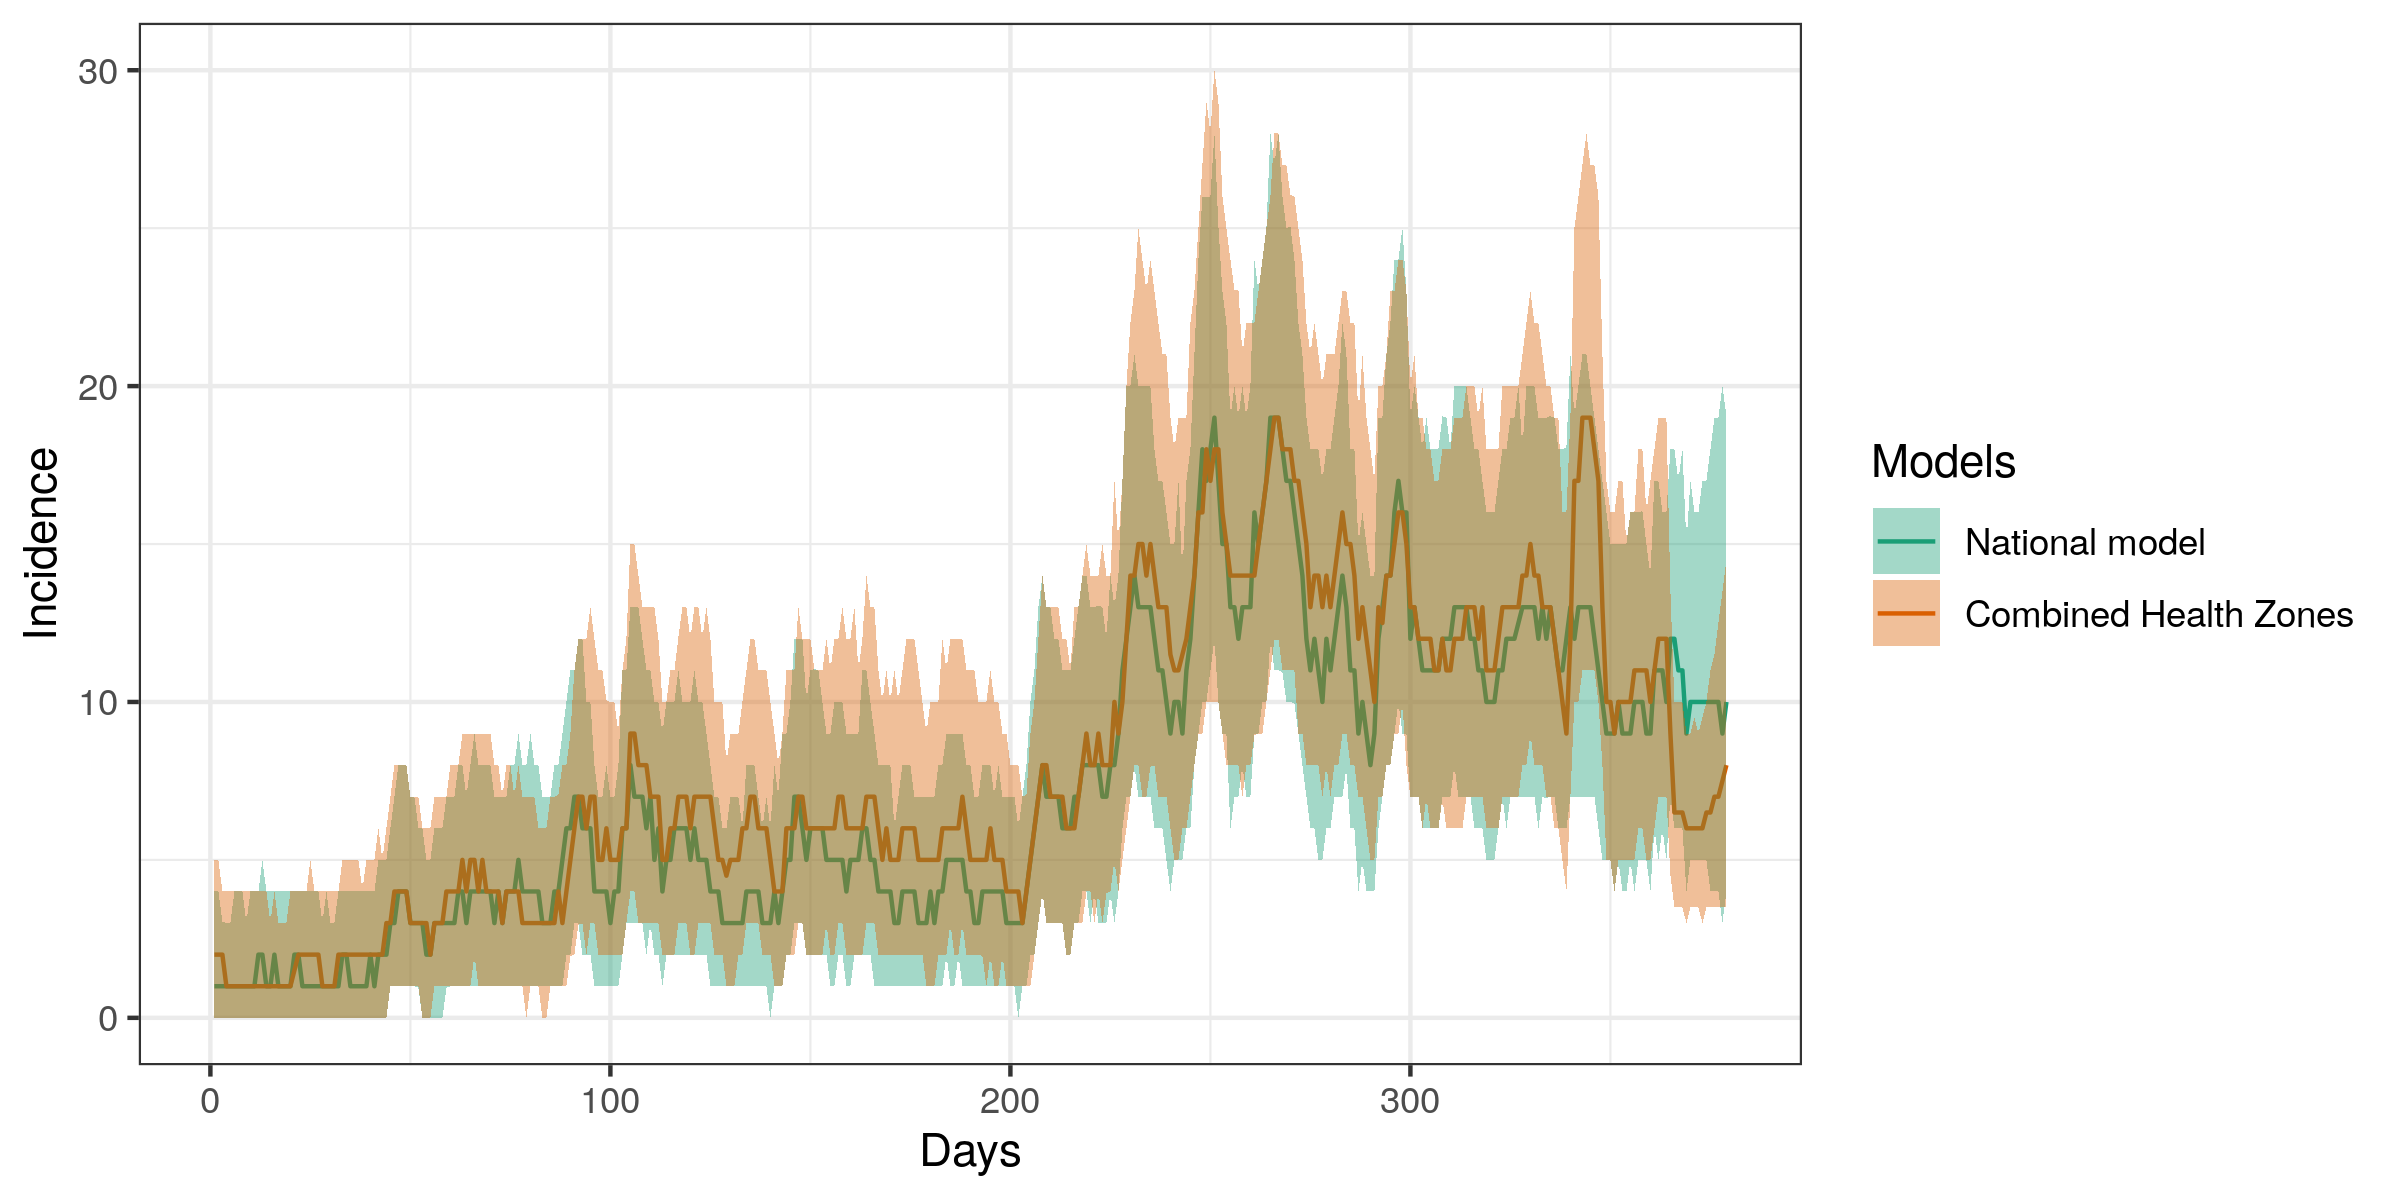
\includegraphics[width=0.9\linewidth]{../output/nat_combined.png}
  \caption{Median and 95\% prediction intervals for one-day-ahead predictions from the Poisson semi-local model for national level compared with the same model when summing up predictions from all health zones.}
  \label{fig:nat_nat_comb}
  
\end{figure}

\section{Discussion}


The ongoing Ebola outbreak in north-eastern DRC is the second largest Ebola outbreak in history and is of significant regional and international concern. As of the 1st of September 2019, the outbreak is not under control, as we can see both from the fact the reproduction number is not below one and that there are still plenty of new cases not on contact lists and multiple community deaths \cite{worldhealthorganisationDiseaseOutbreakNews}. In addition to the large number of confirmed Ebola cases, this outbreak has seen a high CFR of 66\% compared to 51\% in the West African outbreak \cite{rojekSystematicReviewMetaanalysis2019}. Both the long duration, difficulty of control and high CFR are likely due to the difficult context for the outbreak response. The affected area of DRC has a history of violent conflicts and mistrust of the central government and international organisations. This makes all parts of the response from finding cases and tracking contacts to ensuring early treatment and safe burials much more difficult. Based on the models investigated in this paper, it seems that the large increase of cases seen from March to June 2019 is over and there is hope that the outbreak can be controlled. However, the large uncertainty associated with the outbreak which is also reflected in the large uncertainty in the models makes long-term predictions very difficult if not impossible.

Compared to the estimates of the reproduction number in the West African Ebola outbreak \cite{WestAfricanEbola2015}, the reproduction number in the DRC outbreak has seen larger variations on short timescales and less clear patterns over longer timescales. In the previous outbreak, both Guinea and Liberia saw that the reproduction number peaked around two after a few months, followed by a long and slow decline. The current outbreak has been characterised by multiple short-term peaks or waves of higher reproduction number, with the peaks reaching over 3 at certain times. It is possible that the different patterns from the different outbreaks can be explained by the characteristics of the outbreak response. The West African response was slower to get properly started, but once it did, the response was fairly uninterrupted. In the current outbreak, the response had a faster start, but has been interrupted due to the security situation which could explain the short term-peaks in reproduction number. The range of reproductive values seen is also similar to other previous Ebola outbreaks \cite{legrandUnderstandingDynamicsEbola2007}.

We find that on the national level the models with a semi-local trend for the reproduction number were calibrated out to a forecasting horizon of 9 days and significantly outperformed the simpler models based on a non-changing reproduction number. The length of the forecasting horizon is similar, but a bit shorter than the 2 weeks found in \cite{funkAssessingPerformanceRealtime2019}, with a semi-mechanistic model based on a SEIR model that included reporting delays. While direct comparisons are not possible between different outbreaks, it would be of interest if our model with much less deterministic structure can give fairly similar calibrated forecasting horizons. Other models have been used to forecast the current Ebola outbreak, e.g. \cite{kellyRealtimePredictions201820192019, akhmetzhanovAnalyzingForecastingEbola2019}. They use very different modelling techniques, and an appropriate comparison between the models would require comparing proper scoring rules scores using the same data. All the models presented in this paper can easily be run daily on a normal laptop to provide real-time predictions in an outbreak setting. 


The best model for the national outbreak is uncalibrated when forecasting more than 9 days forward because it overestimates the amount of uncertainty in the incidence. Depending on how the forecasts are used, it is possible that uncalibrated but over-dispersed forecasts can still be useful for planning purposes since they are conservative. An upper limit for an over-dispersed forecasts will give a conservative upper limit for future incidence. Forecasts based on under-dispersed models require a lot more care and should be treated with caution. Models that only provide point predictions or do not actively try to quantify the uncertainty are by definition underdispersed. The main reason for the over-dispersion in the semi-local models is likely the forecasting of the reproduction number. This model allows a large variation in the reproduction number over a fairly short time, but does not have any information about what range of reproduction numbers is actually feasible. In this outbreak we see fairly fast changes of the reproduction number, but the reproduction number is almost never larger than three. A model for the reproduction number than allows this fast variation and short peaks, but keeps the reproduction number within a more narrow band, might provide better forecasts.

To compare foreacasts and evaluate models for probabilistic forecasts, tests for calibration and the use of proper scoring rules is a crucial. The proper scoring rules are mainly useful for model comparissons, while the calibration gives an absolute measure for how well the forecast captures the uncertainty seen in the process. In this study, we found these tools crucial both for model selection and for the final interpretation of our model. Even a well calibrated model can make large forecasting errors if the underlying process changes in a way not seen during the time period used to fit and evaluate the model. Therefore it is always crucial to evaluate critically both the models and the metrics used to evaluate the models. We find that both the RPS and DSS scores give similar conclusions, but that calibration using the PIT values was especially valuable as an absolute measure of calibration. The introduction of the centrality measure of the PIT histograms gives additional valuable information and allows us to understand better how our models are failing if they are not well calibrated. The centrality is a fairly crude measure of this, and measures that also include other departures from uniformity of the PIT values could give additional information. 

We find that for one-day-ahead forecasts the negative binomial distribution is needed for a calibrated forecast. This indicates that a Poisson offspring distribution where everyone is always equally likely to transmit the disease in every small time step does not adequately describe the transmission process. We found a relatively large value for the $k$ parameter which gives a fairly modest increase in the variance, or degree of superspreading This increase in variance is much smaller than what was found when investigating transmission chains in the West African Ebola outbreak \cite{internationalebolaresponseteamExposurePatternsDriving2016}. It is possible that the variance is smaller in this outbreak, but this study should be taken as fairly weak evidence and a proper investigation of transmission chains would be needed. 

We could provide forecasts for all health zones with more than one case, but the quality was varying. For some health zones where there were very few cases and then a longer period with no transmission, the model managed fairly well, but for most health zones with a large number of cases the models were again too over-dispersed to provide calibrated predictions. Once our model has seen no new infections in a few weeks, it will predict close to zero new cases with essentially zero sharpness, irrespective of the current reproduction number. This behaviour works well when there are no new imported cases, as we can see in some of these health zones. Some of the well calibrated health zone forecasts only saw their first Ebola case quite late in the outbreak, giving many fewer data points to test the model. This can make it hard to reject calibration even if the model is uncalibrated. For almost all health zones, the models with semi-local trend were better than the models with a constant reproduction number. This was also the case when we combined all the forecasts from all the health zones where the combined RPS showed that the semi-local-trend models performed significantly better. Overall, the health-zone-level forecasts were not well calibrated when we combined the PIT values or when we aggregated the forecasts to compare against the national level incidence. It is clear that our model works much better on the national than the sub-national level.  

%% Model assesment


The models and forecasts in this report have multiple limitations. First, using a data source that only includes daily updated cumulative case counts has many disadvantages compared to a line list of all cases. A line list would give a much more accurate data on of the date of the onset of disease, and it would remove the problem with negative incidence rates after corrections and any problems with having to interpolate incidence rates. It is a strength of the modelling approach that it can be used on less than ideal data and still give reasonable short-term forecasts. The stringent tests of calibration can give us confidence in the forecasts even without perfect data. This is of key importance in outbreak situations where having up-to-date line lists of cases can be difficult or impossible. In these situations, we could still hope that the approaches in this report could give reasonable forecasts. 

The models in their current form also have several limitations. As previously discussed, the semi-local-trend models seem to predict too much variance in the reproduction number which leads to over-dispersed predictions. There are also clear limitations when the models are used on the health-zone level since the spread between health zones is not modelled. Each health zone is modelled independently as if it were the whole outbreak. We only model the spread of the disease after it has been introduced to a health zone. It is possible that this is partly the reason for the uncalibrated forecasts on the health zone level. At he national level we do not have this limitation, but it makes it very difficult to use the current model to study the spatial spread of the disease. Due to the flexibility of the model structure, it would be fairly straightforward to improve the models by incorporating an additional force of infection term that gives the force of infection from outside the health zone. There are multiple options for how to model the spatial dependence that would all easily fit into our model structure. This includes spread from adjacent health zones, using a gravity model where the amount of spread between health zones is based on the populations \cite{haynesGravitySpatialInteraction1985} or, if available, data on travel between health zones could be used. Without this spread term, the model cannot be used to forecast probabilities for the spread of Ebola to new health zones. In addition, the current way of estimating the time-varying reproduction number requires at least 17 days of data, which means that we need at least 17 days of data in a health zone to be able to forecast.

In addition to improvements related to the spatial spread, it would be beneficial to combine the separate parts of the model into one generative model. This means that the estimation of the reproduction number could be included into the modelling of the incidence. One promising way of doing this is a full Bayesian generative model. One of the main benefits of a generative model is that it models the whole data generation process and would allow us to simulate whole outbreaks. For future work, it would also be very interesting to investigate different models for the time evolution of the reproduction number. A full Bayesian treatment would also allow us to model uncertainty in the parameters of the offspring distribution and in the serial interval. It could even include imputation for missing data using the general modelling framework presented here.

In this report we used a semi-mechanistic model with fairly few assumptions about the exact mechanism of disease transmission. The flexibility of the reproduction number in this model allows us to fit complicated incidence histories that could not have been easily fit by traditional compartmental models. The benefit of the structure we do have in the model is that we ensure that the model correctly models certain basic facts about the outbreak like the serial interval and that all the parameters are interpretable. More structure is likely to make the model better if the assumptions in the model are true, but will often make it impossible to get a good fit when assumptions are wrong. The basic structure included in our models is also likely to describe a large number of other infectious diseases. Therefore, they could easily be adopted to other diseases and other contexts without any real changes in the model structure. We would need a different serial interval, but the rest of the model could be used as it is. Another benefit of adding more structure to a model, for example a SEIR structure is that it is easier to model the results of interventions like vaccination\footnote{Using the fact that $R_t=R_o*s(t)$ in a compartmental model of the SEIR type, it would likely be possible to also model some simple interventions in the models considered in this report.}. One key aspect to consider when choosing models for an outbreak situation is that perhaps more than one model should be used during the outbreak. At the start of the outbreak when the important mechanisms of disease transmission and population behaviours are less well known, a model with less mechanistic structure is perhaps the most useful. Once we learn more about the outbreak, we can add more structure to the model. In many forecasting challenges it has been shown that an ensemble of models performs better than individual models \cite{dietterichEnsembleMethodsMachine2000, yaoUsingStackingAverage2018}. This was also found in the RAPPID modelling competition for Ebola \cite{viboudRAPIDDEbolaForecasting2018}. Therefore, combining multiple models with different strengths could give a better overall forecast. For example, a combination of the negative binomial model with a constant reproduction number, which did well for early forecasts, with the Poisson semi-local model, which did better for slightly longer forecasts, could give an even better model.

Theoretically it should be possible to forecast infectious disease outbreaks on the timescale of individual outbreaks \cite{scarpinoPredictabilityInfectiousDisease2019}. The models in this report and other disease forecasting models still have a long way to go to achieve this goal. For the current Ebola outbreak ther are many additional sources of data that are not curently used in our models. These includes deaths, community deaths versus deaths in treatment centres, contacts followed up, vaccinations, data on response activities etc. It is possible that combining these additional data sources together with improved modelling techniques we could significantly increase forecasting horizon where we can provide calibrated predictions. 





\section{Conclusions}
We presented a probabilistic disease modelling and forecasting framework based on a modified branching process with a time-varying reproduction number. When we modelled the reproduction number with a semi-local trend, the models could give well calibrated forecasts for the 2018--2019 Ebola outbreak in DRC for forecasting horizons of nine days. The models provide easy-to-interpret forecasts of incidence and reproduction number. They could could also provide good incidence forecasts for some health zones at the sub-national level. At both the national and the sub-national level, forecasts based on a constanct reproduction underestimated the uncertainty and forecasts based on a semi-local trend for the reproduction number overestimated the uncertainty at longer forecasting horizons. 


\newpage

\bibliography{bibliography} 
\bibliographystyle{unsrturl}

\clearpage
\newpage

\appendix
\appendixpage
\addappheadtotoc
\addtocontents{toc}{\protect\setcounter{tocdepth}{0}}
This appendix shows the best fitting model and evaluation score for each health zone.

 \section{ Butembo }\begin{figure}[H]\begin{subfigure}{\textwidth}  \centering  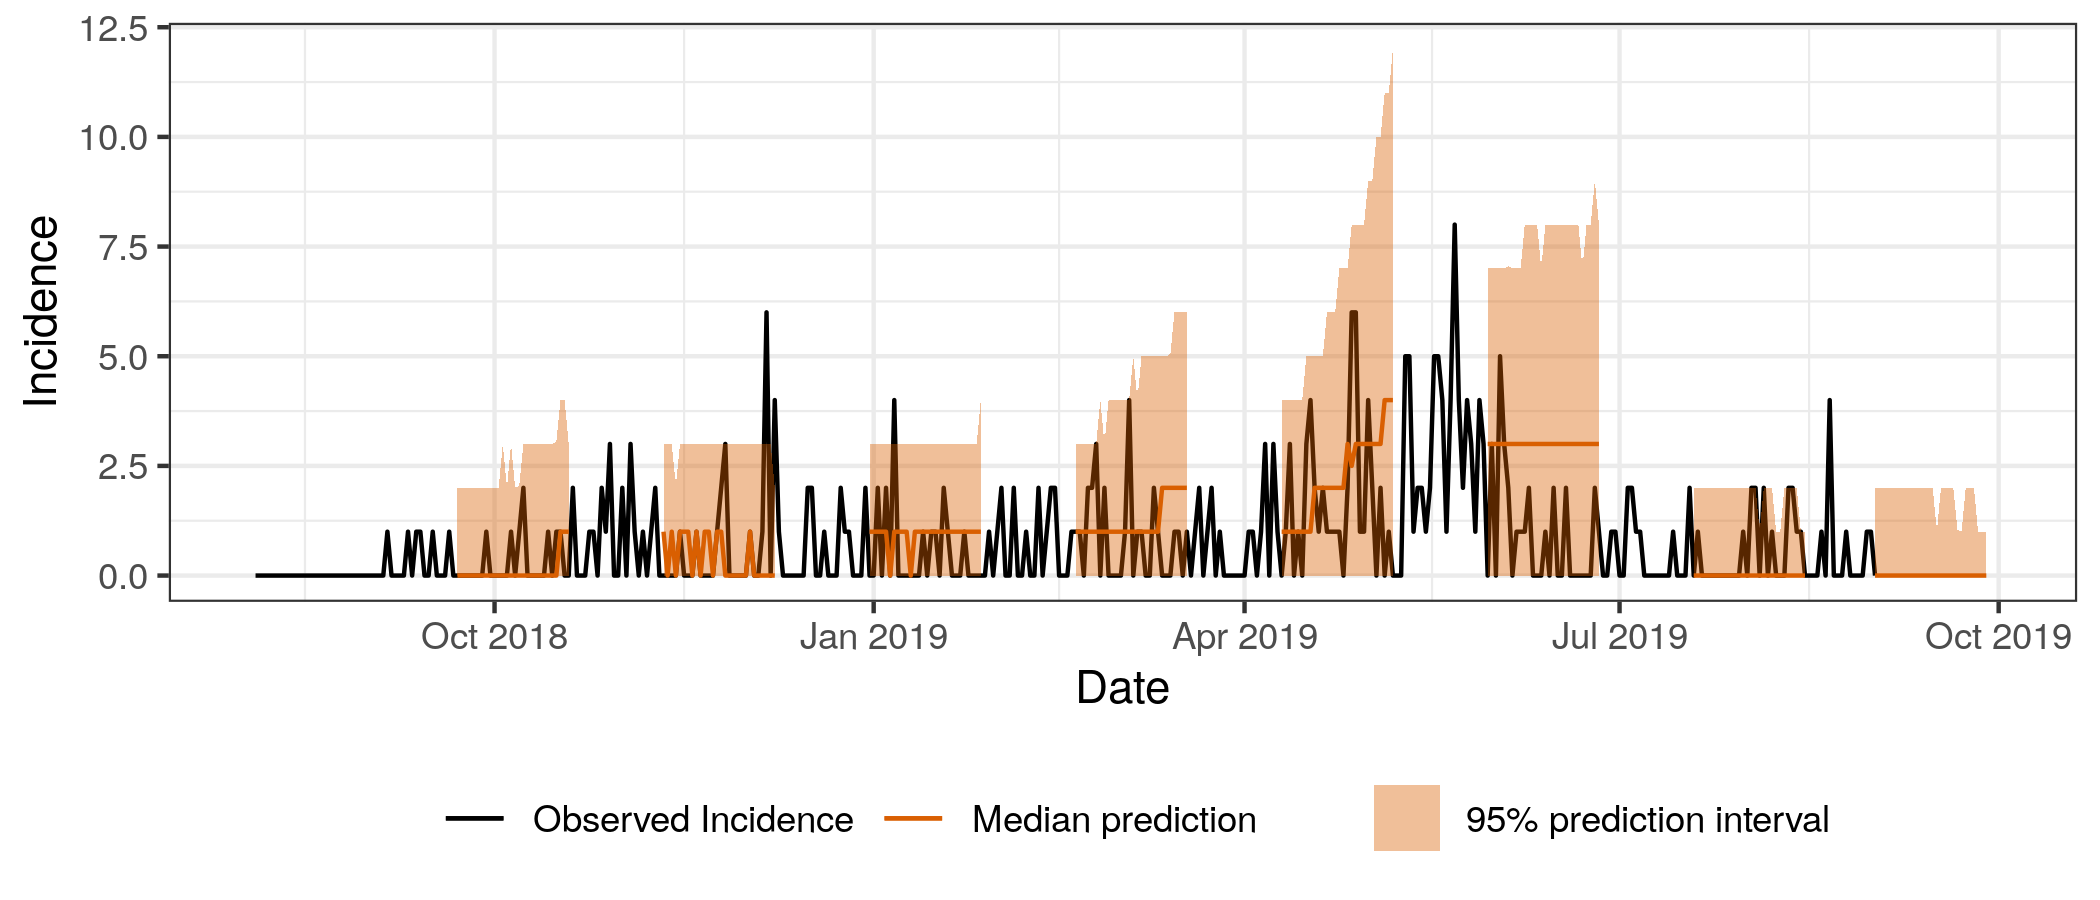
\includegraphics[width=0.9\linewidth, height=7cm]{../output/Butembo_predictions.png}  \caption{Forecasted and predicted incidence for the best fitting model}\end{subfigure}

\begin{subfigure}{\textwidth}  \centering  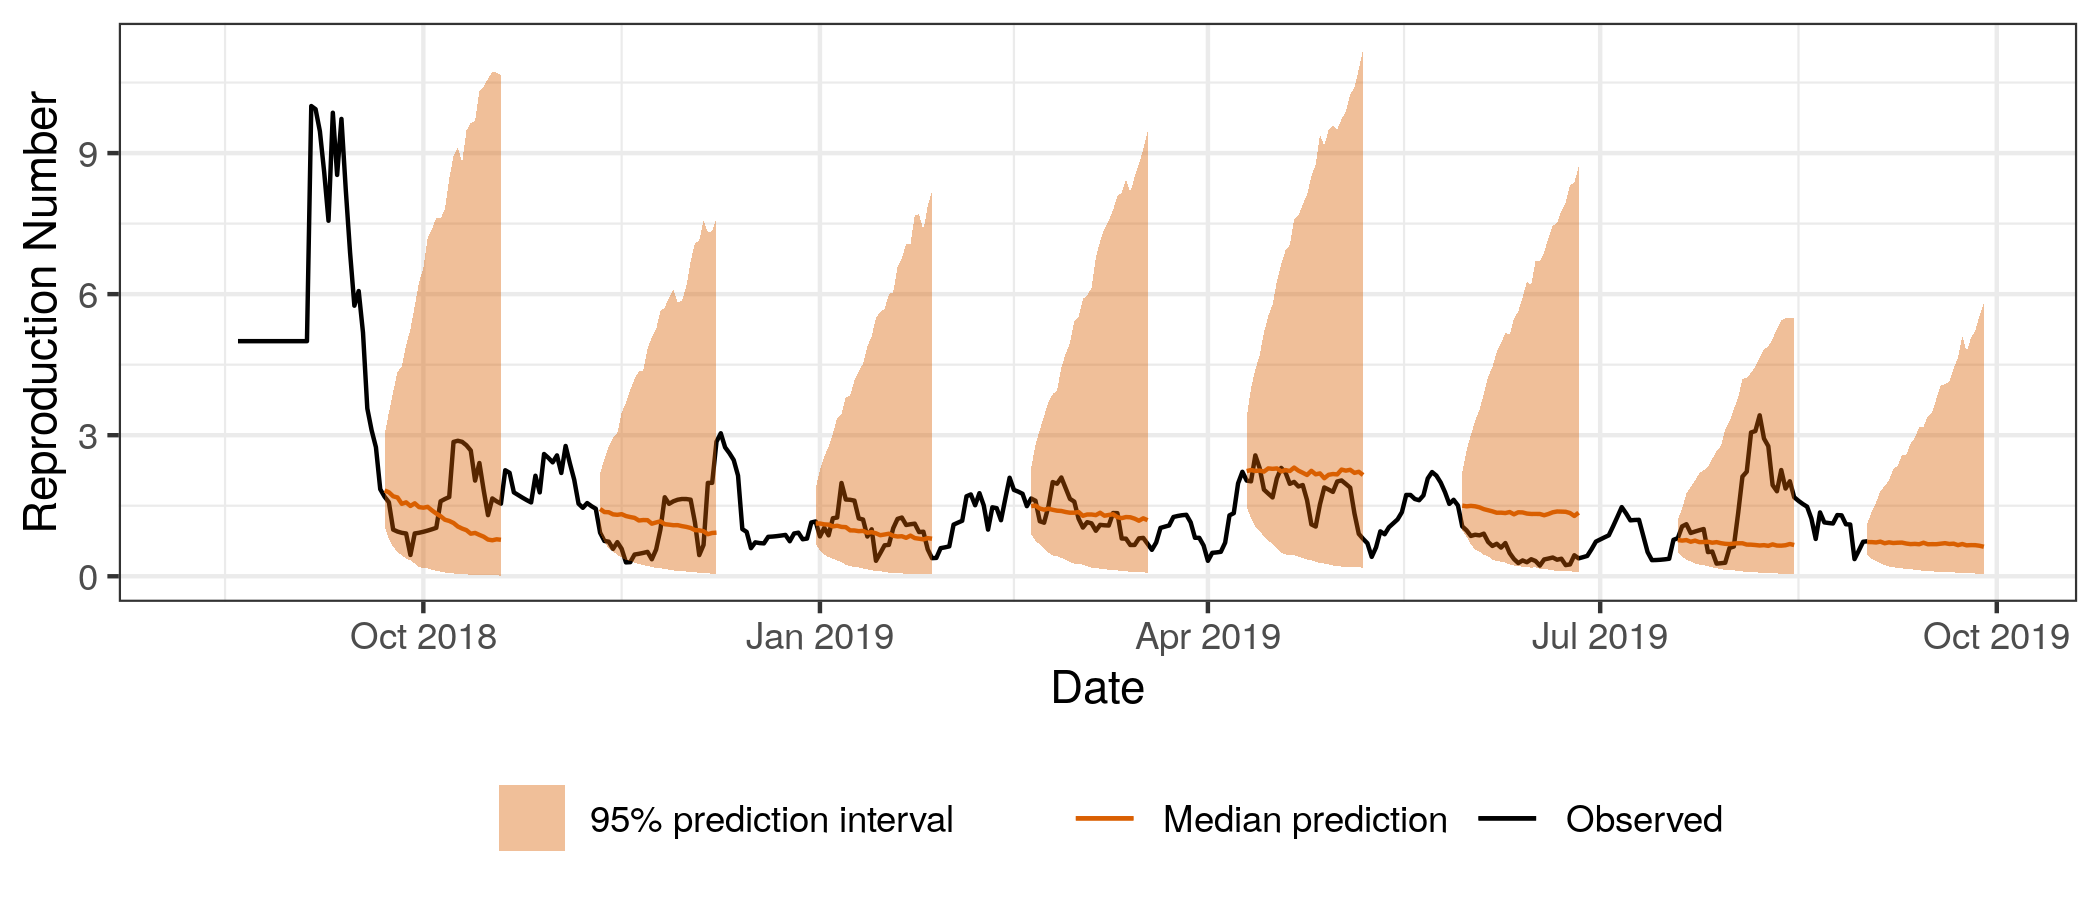
\includegraphics[width=0.9\linewidth, height=7cm]{../output/Butembo_Rs.png}  \caption{Forecasted and predicted repreoduction numbers for the best fitting model}\end{subfigure}  \caption{Median forecast with 95 \% prediction intervals and observed values for incidence and reproduction number for the best fitting model for Butembo.}\end{figure}

\begin{figure}[H]
\begin{subfigure}{0.5\textwidth}
  \centering
  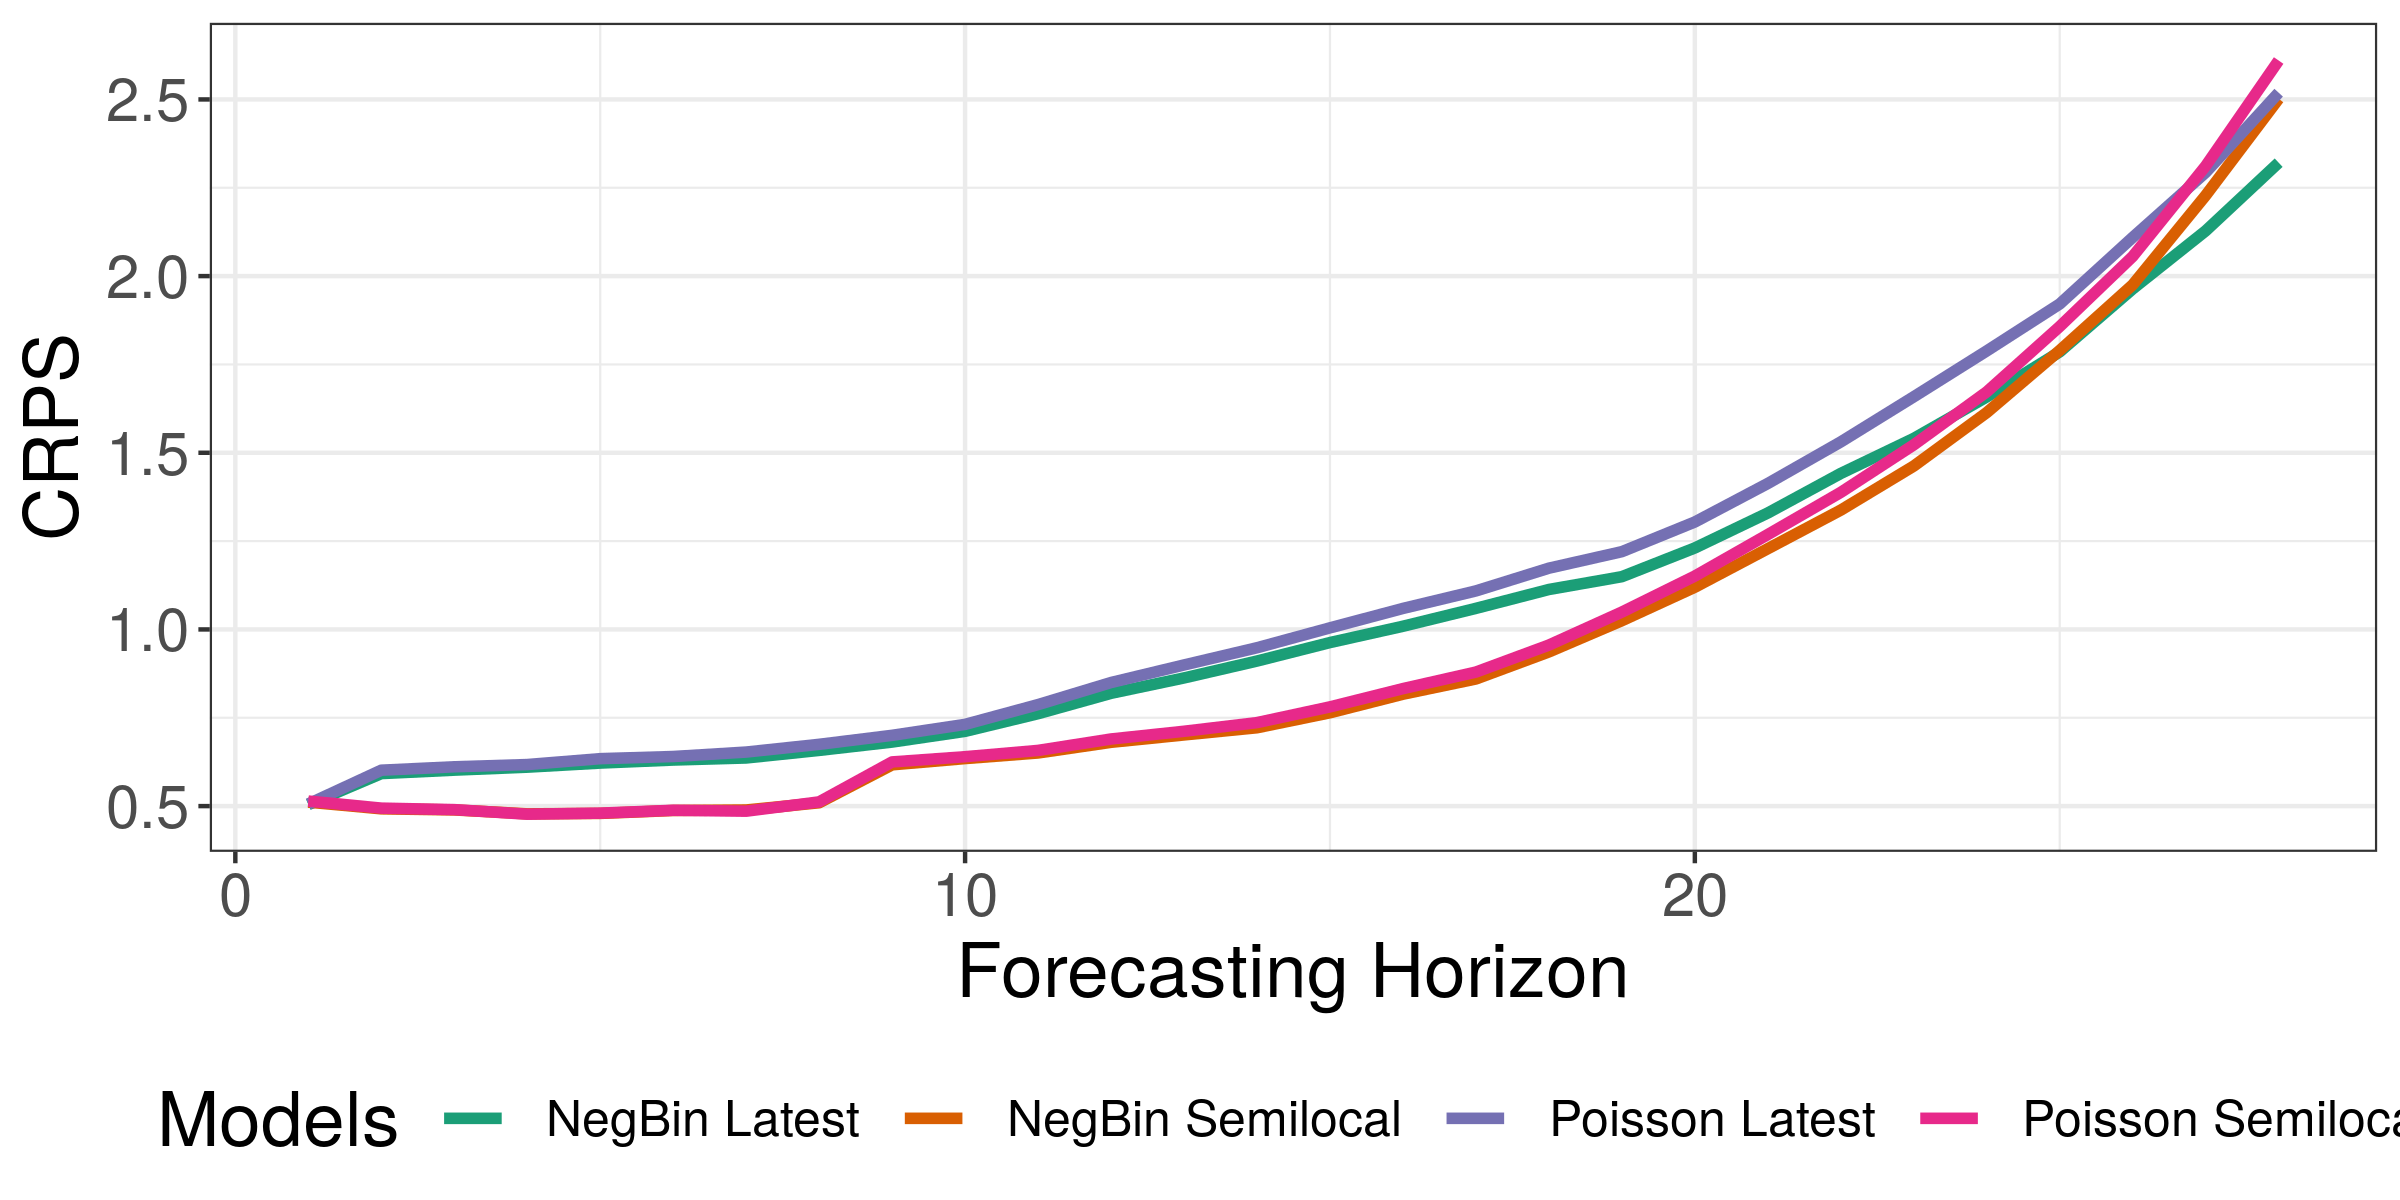
\includegraphics[width=\linewidth]{../output/Butembo_crps.png}  
  \caption{Contineously Ranked Probability Score}
  \label{Butembo_scores_1}
\end{subfigure}
\begin{subfigure}{0.5\textwidth}
  \centering
  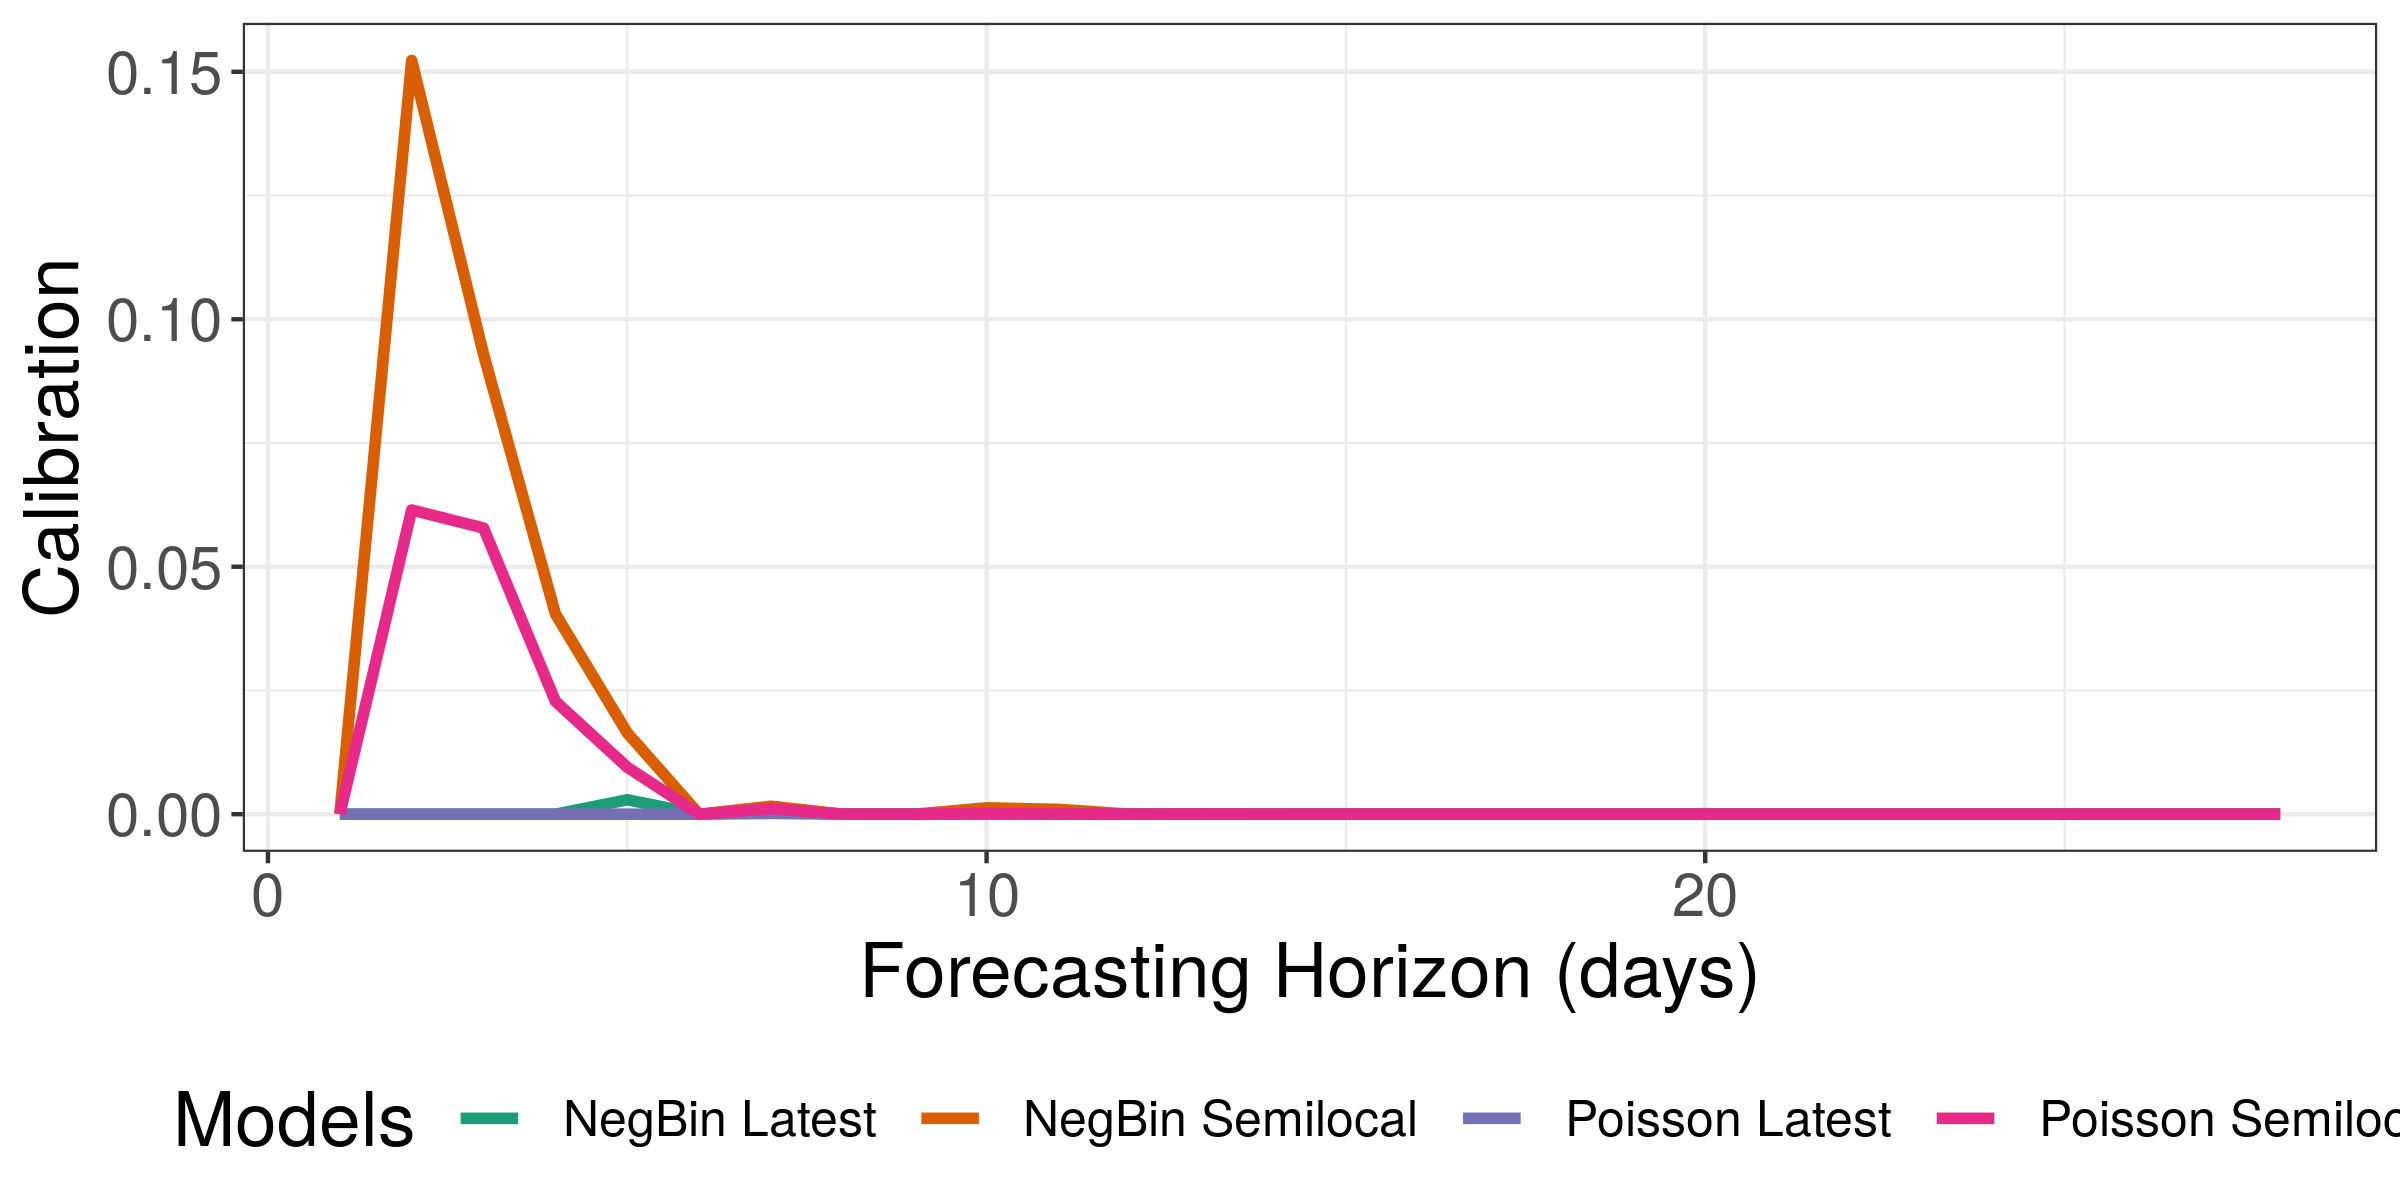
\includegraphics[width=\linewidth]{../output/Butembo_calibration.png}  
  \caption{Calibration p-value}
  \label{Butembo_scores_2}
\end{subfigure}

\begin{subfigure}{0.5\textwidth}
  \centering
  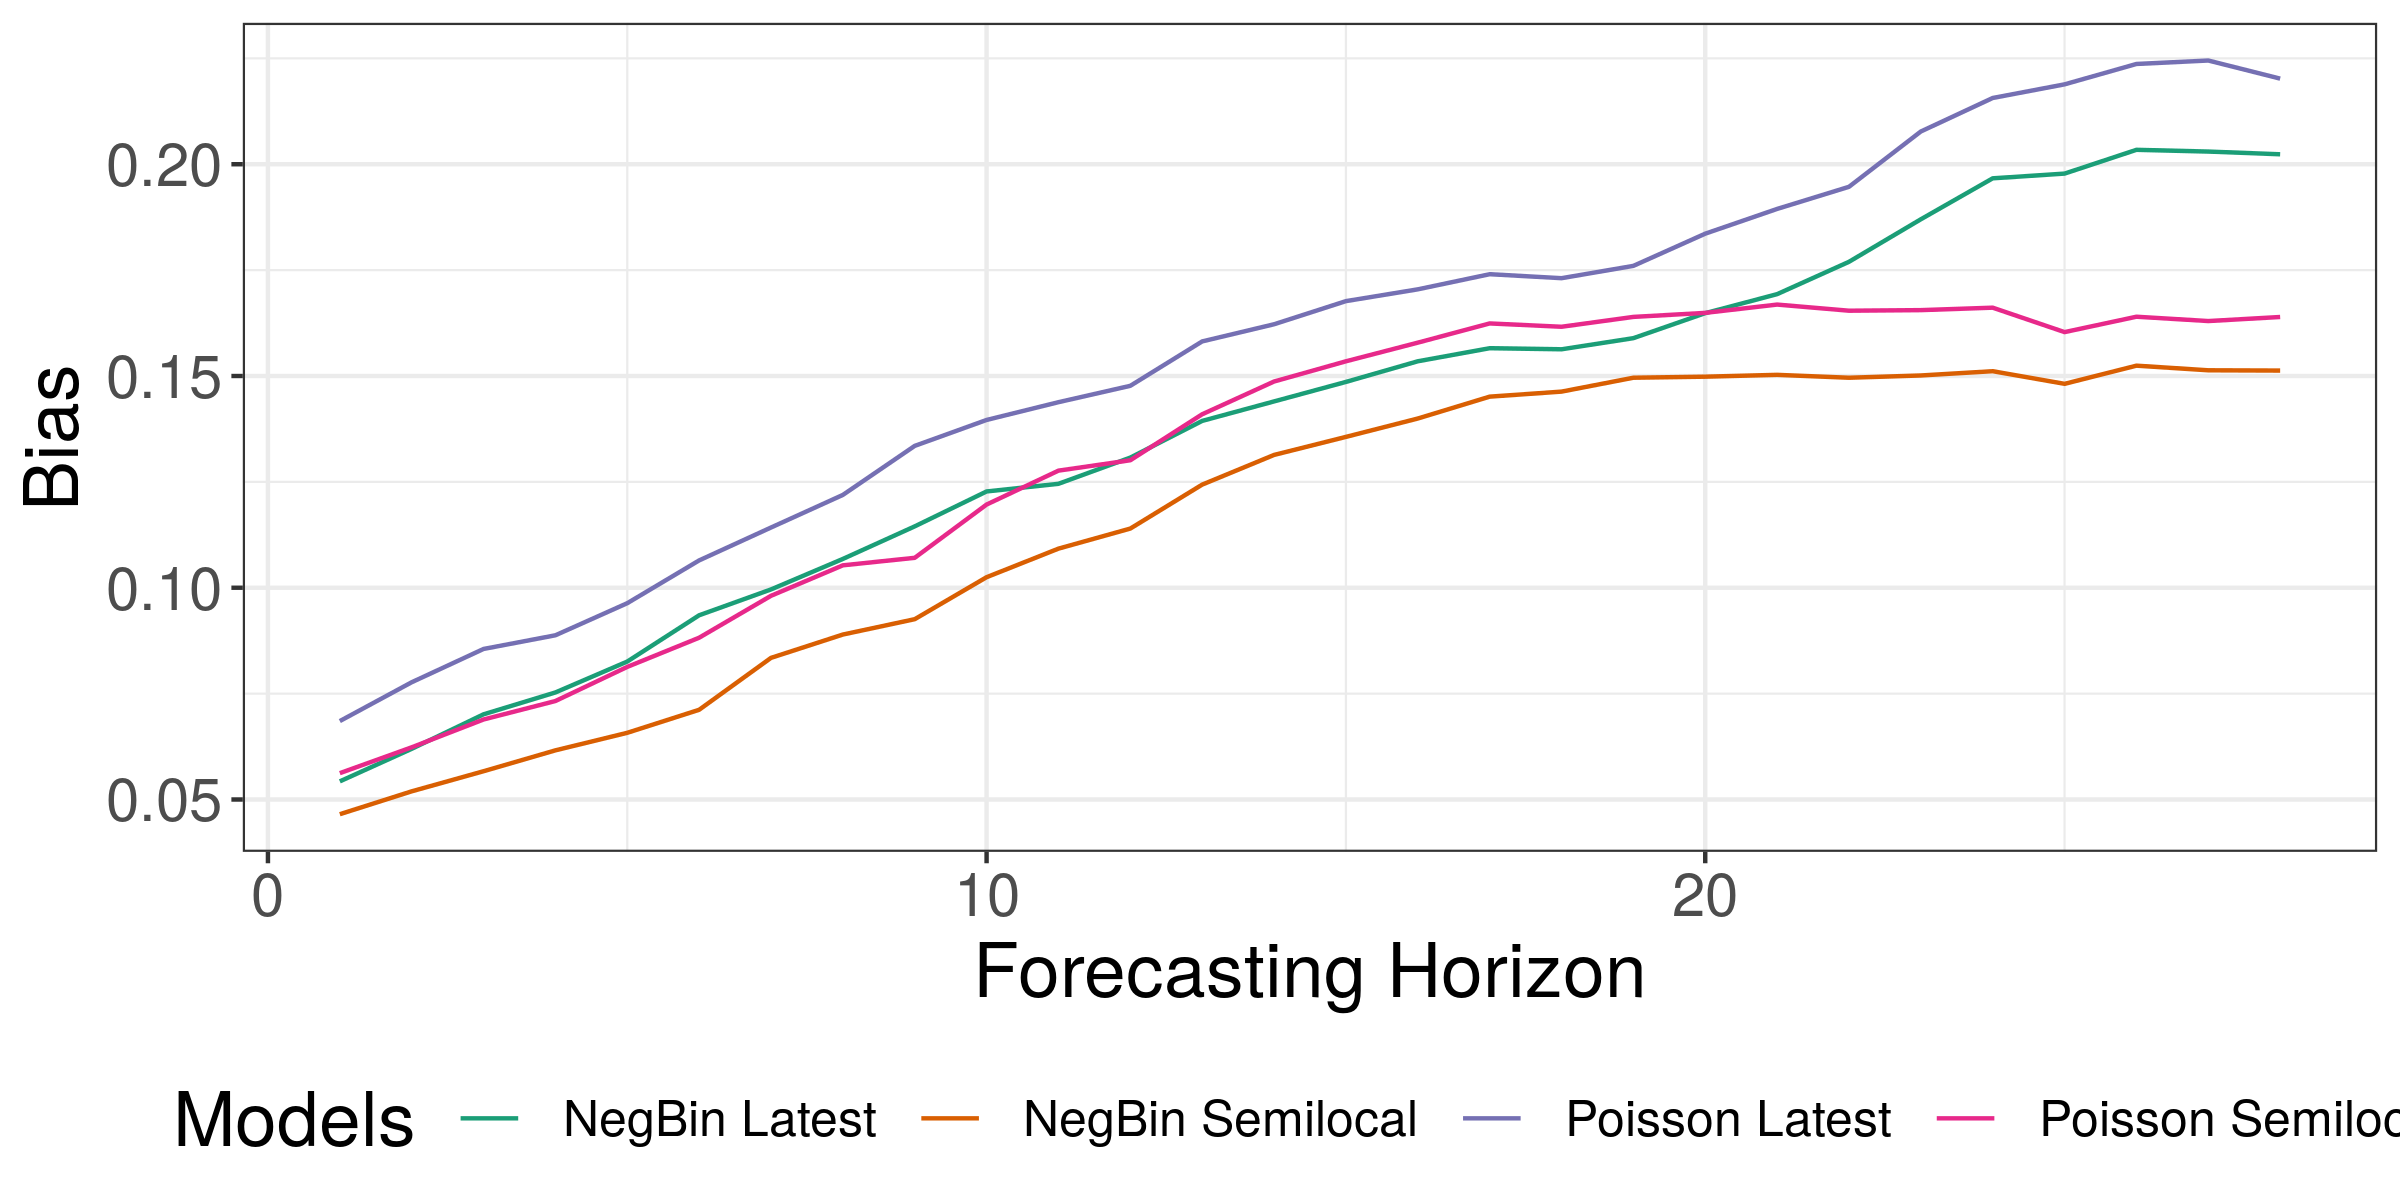
\includegraphics[width=\linewidth]{../output/Butembo_bias.png}  
  \caption{Bias}
  \label{fig:Butembo_scores_3}
\end{subfigure}
\begin{subfigure}{0.5\textwidth}
  \centering
  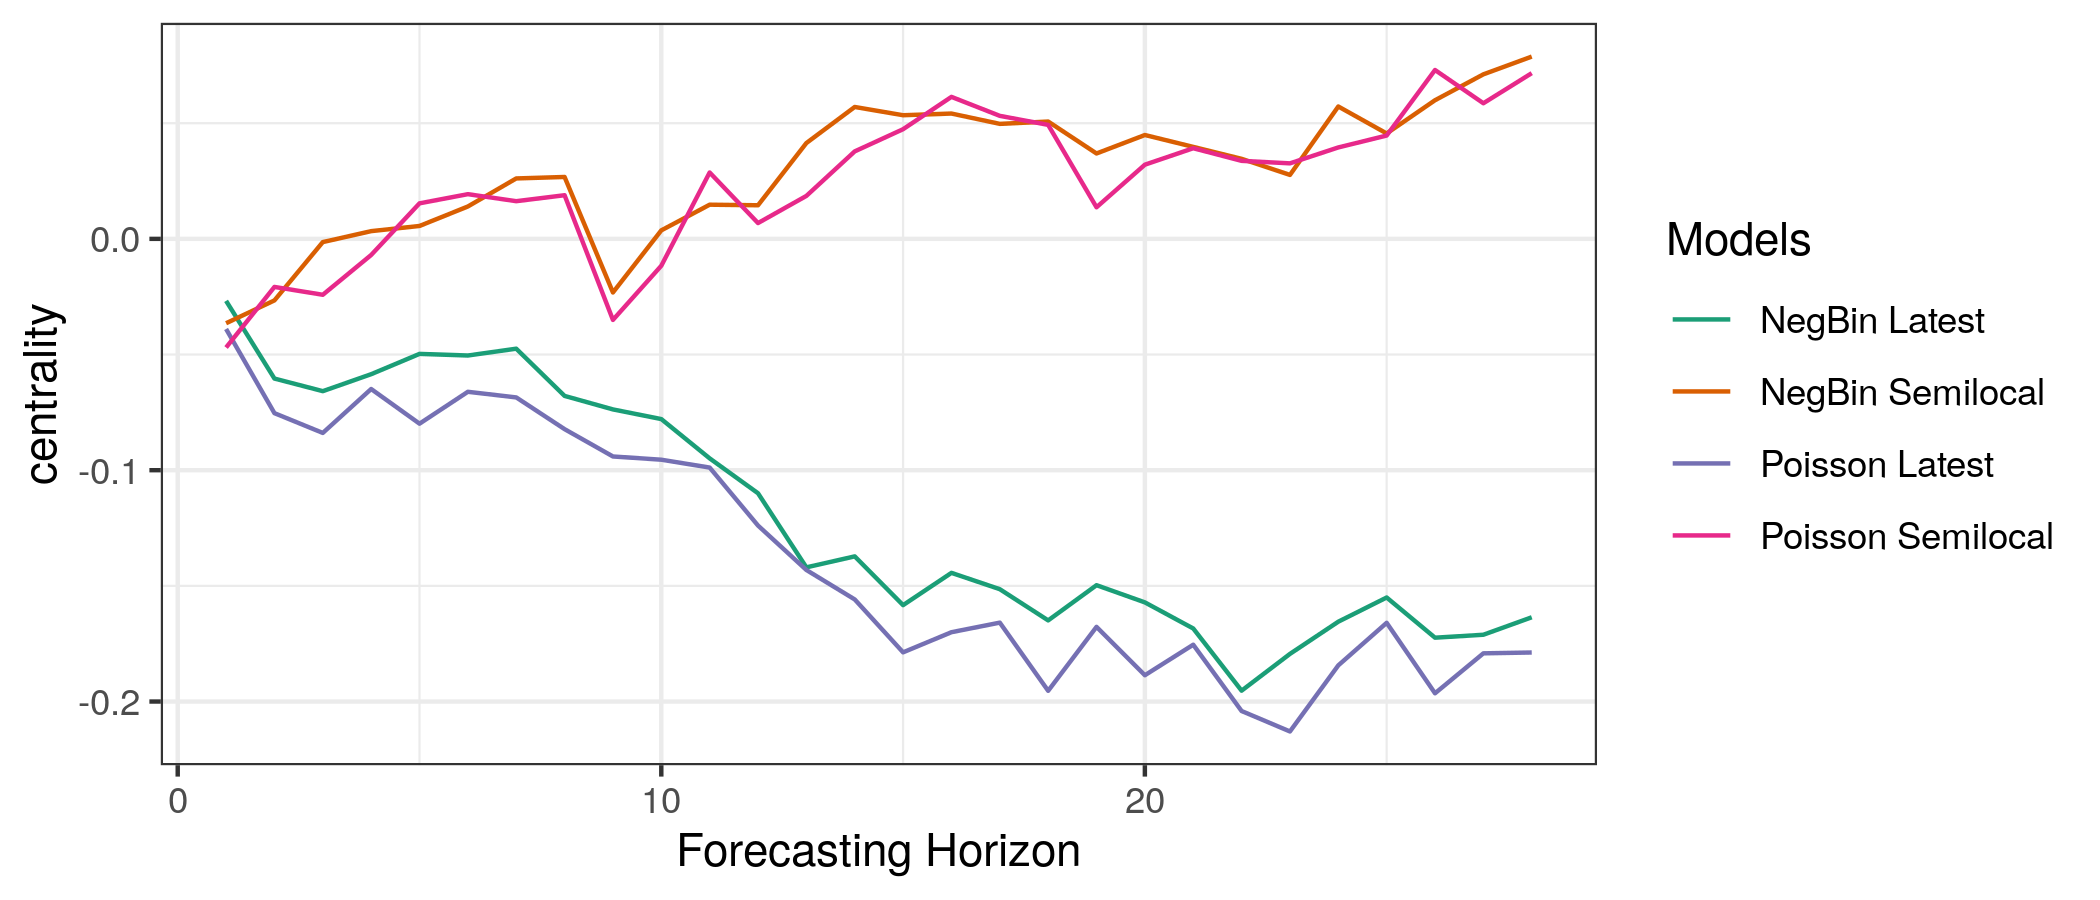
\includegraphics[width=\linewidth]{../output/Butembo_centrality.png}  
  \caption{Centrality of PIT values}
  \label{fig:Butembo_scores_4}
\end{subfigure}
  \caption{Scores for Butembo as a function of the forecasting horizon.}

  \label{fig:nat_scores}
\end{figure}
 \section{ Mabalako }\begin{figure}[H]\begin{subfigure}{\textwidth}  \centering  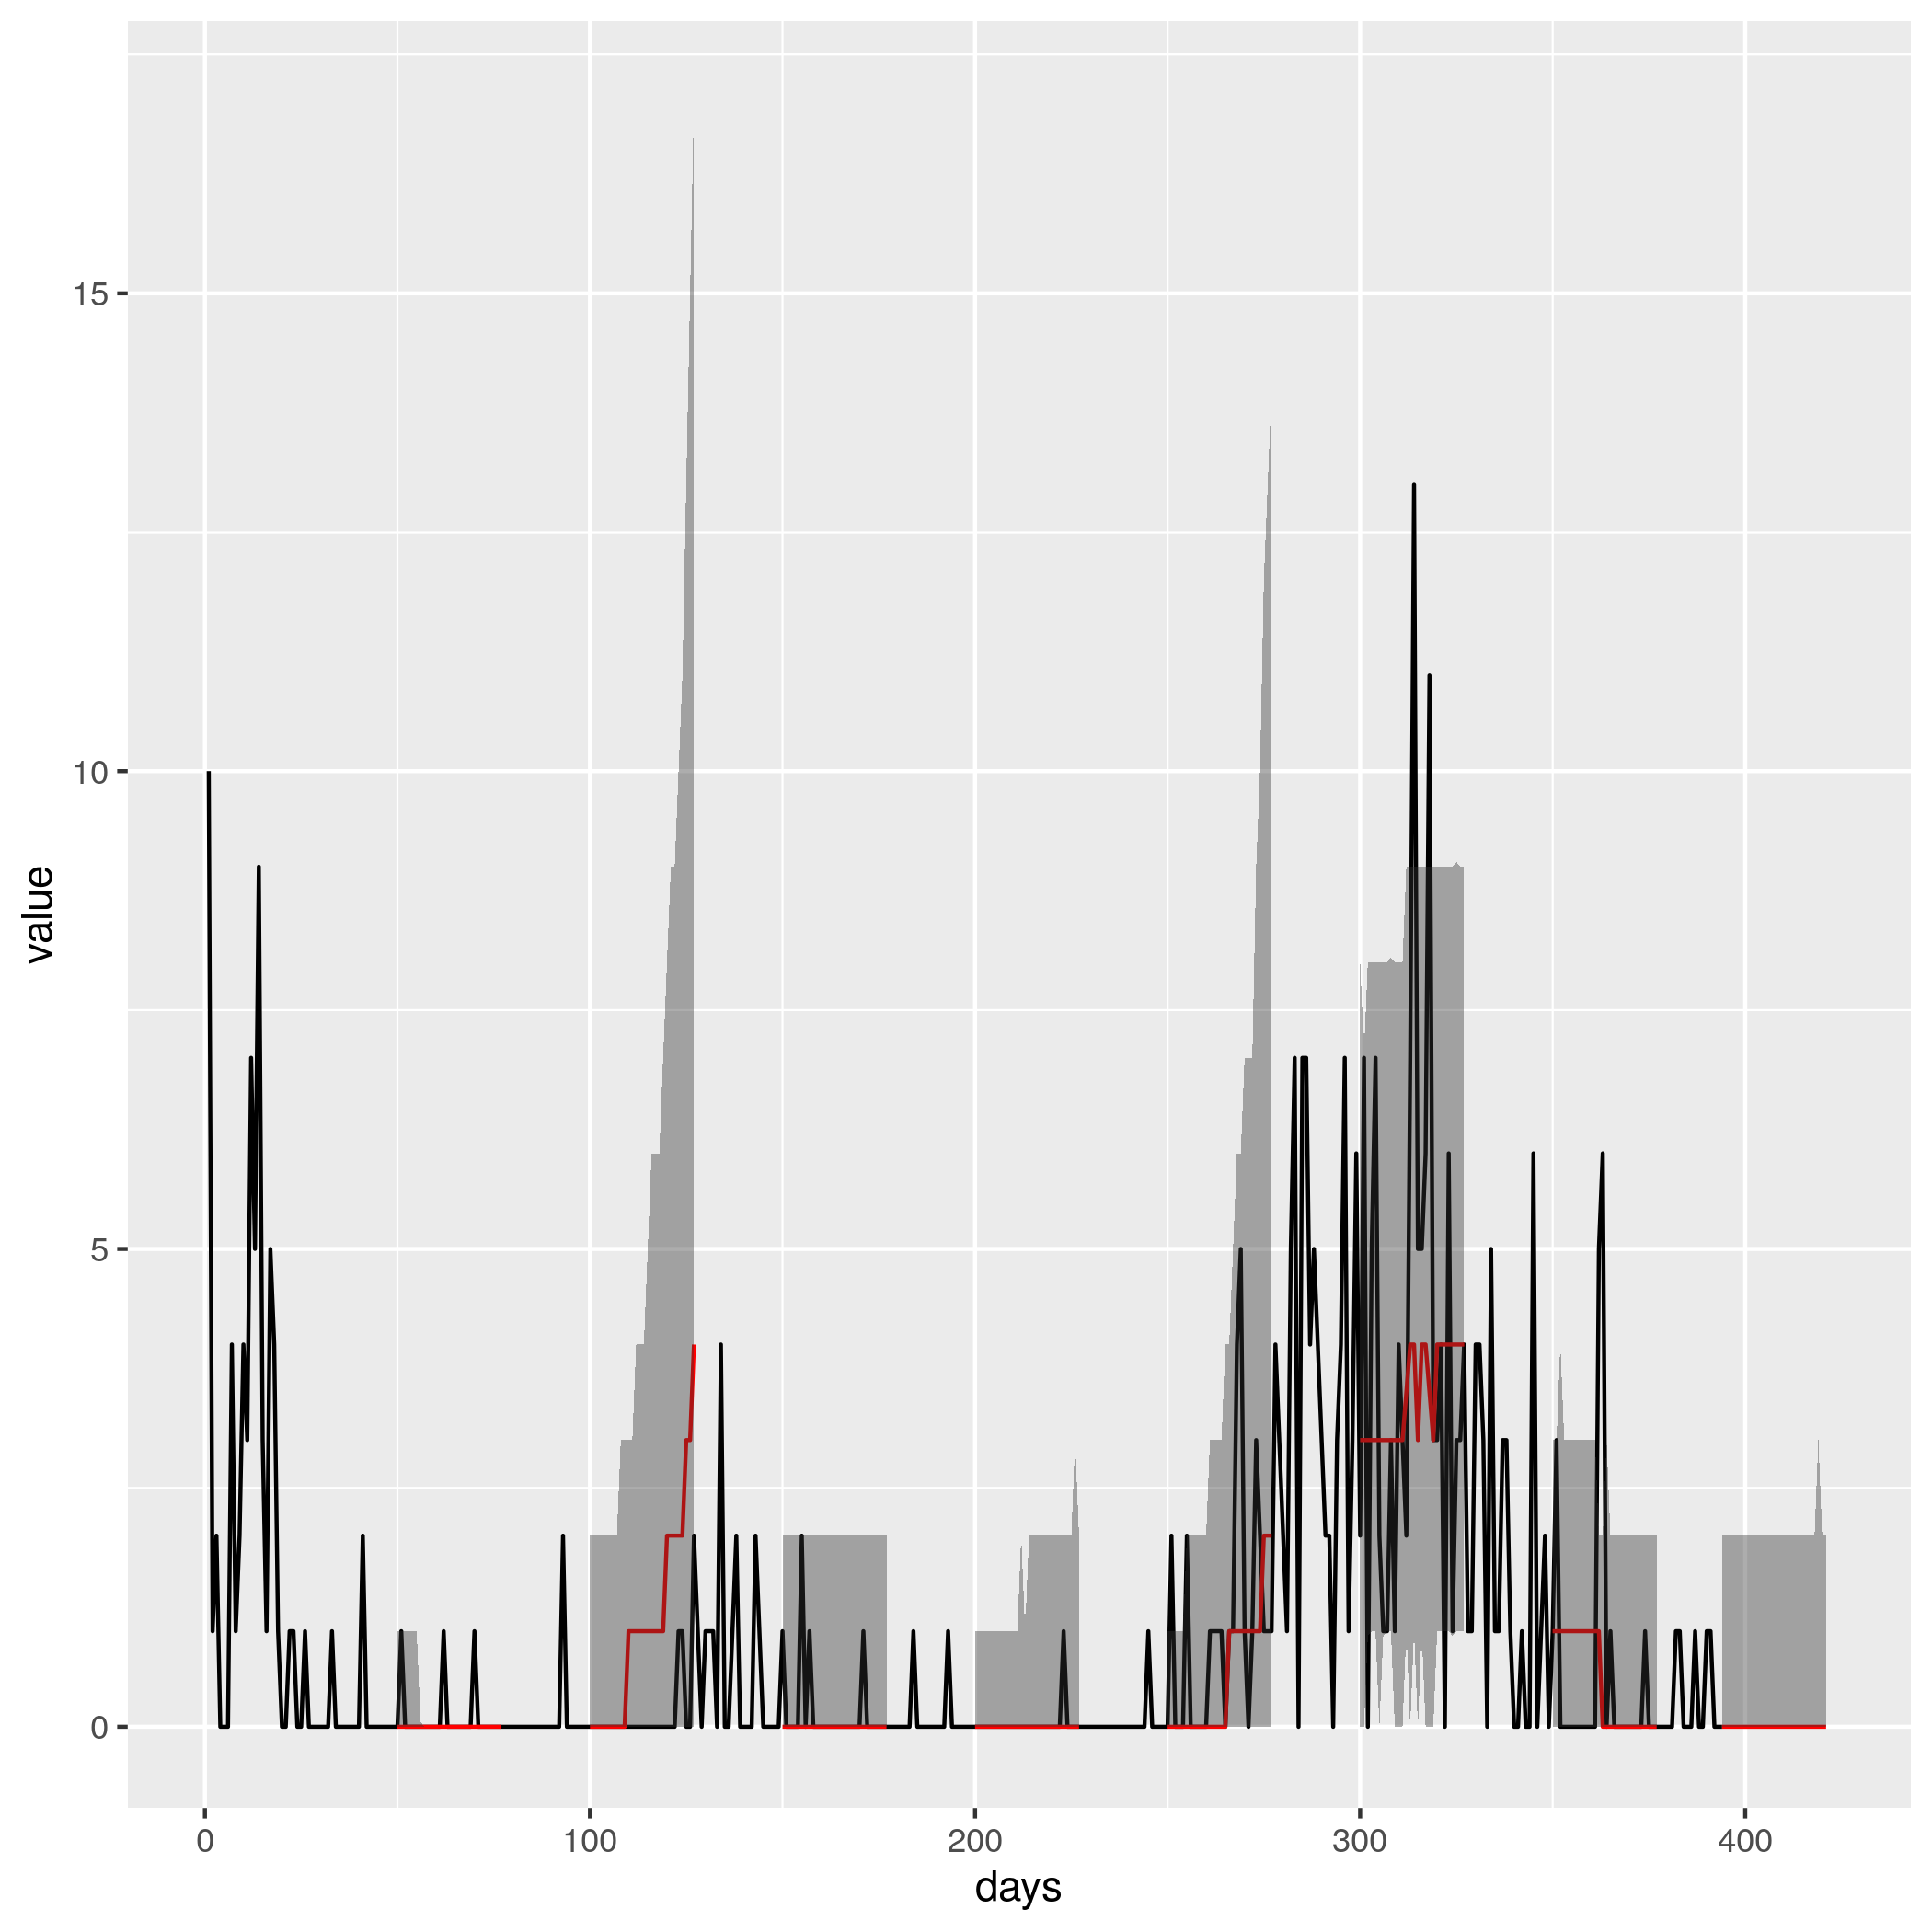
\includegraphics[width=0.9\linewidth, height=7cm]{../output/Mabalako_predictions.png}  \caption{Forecasted and predicted incidence for the best fitting model}\end{subfigure}

\begin{subfigure}{\textwidth}  \centering  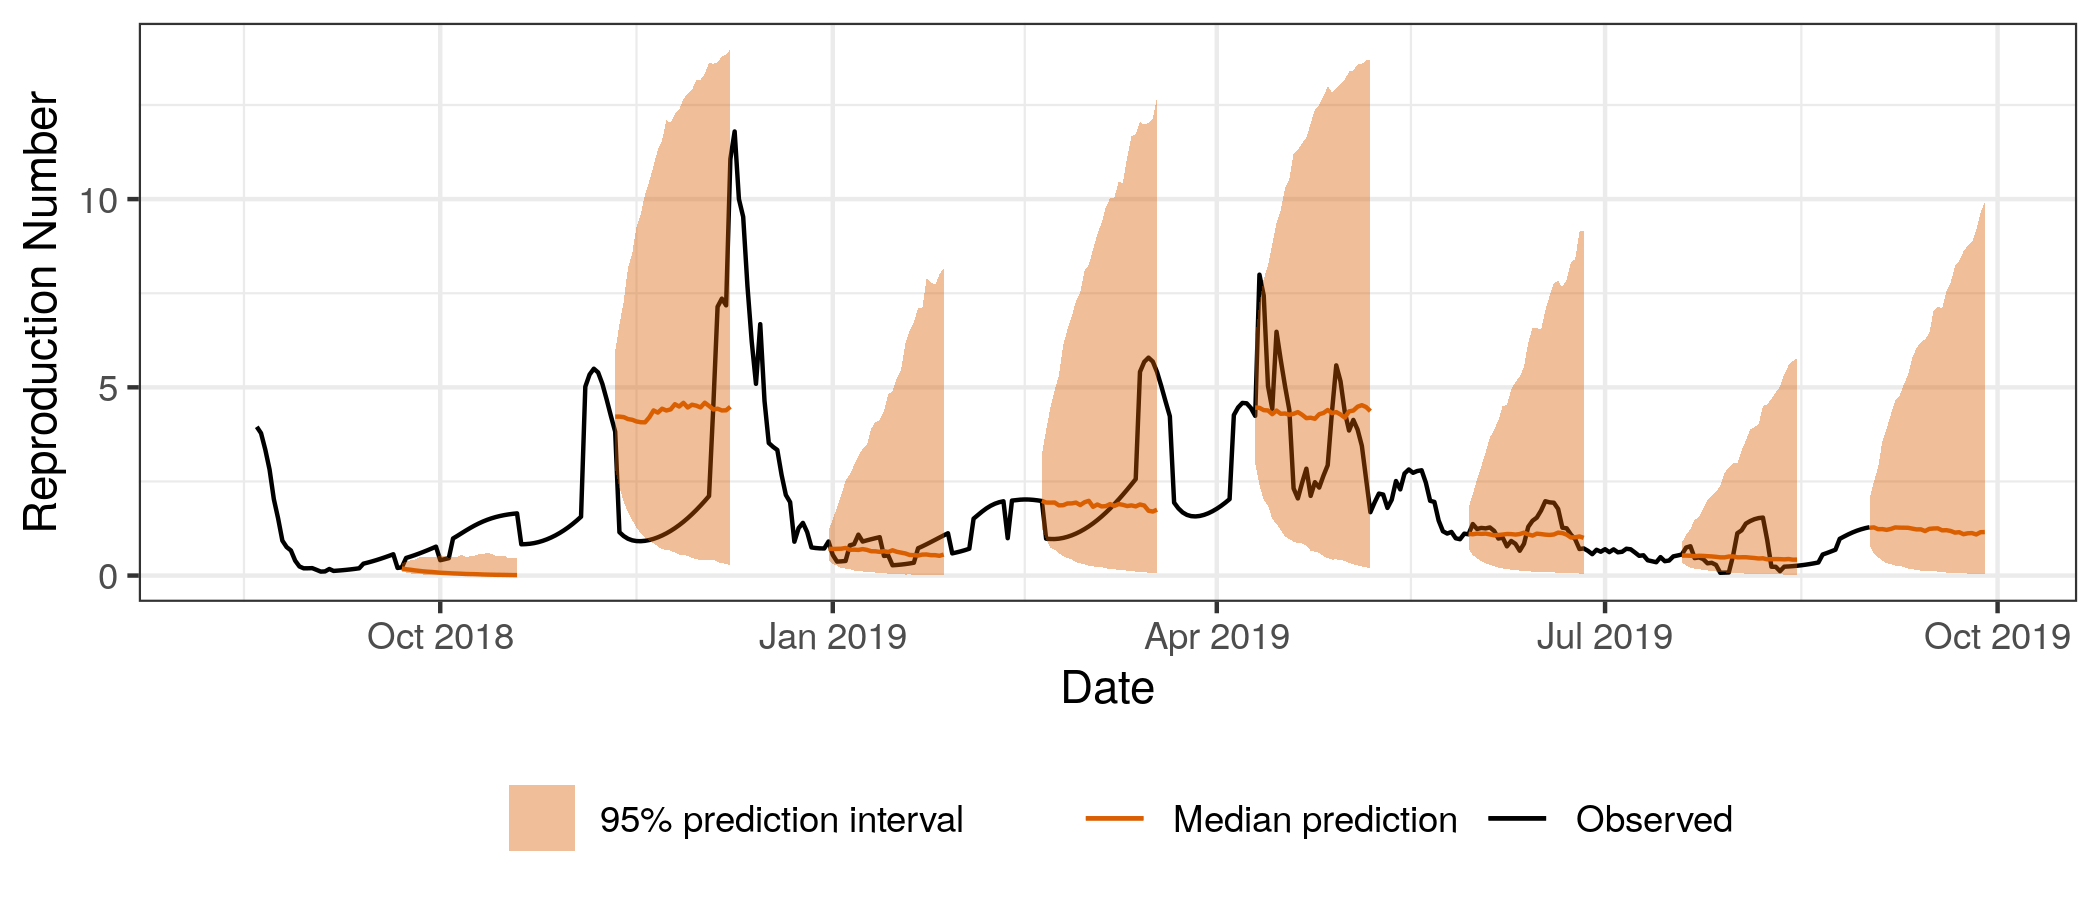
\includegraphics[width=0.9\linewidth, height=7cm]{../output/Mabalako_Rs.png}  \caption{Forecasted and predicted repreoduction numbers for the best fitting model}\end{subfigure}  \caption{Median forecast with 95 \% prediction intervals and observed values for incidence and reproduction number for the best fitting model for Mabalako.}\end{figure}

\begin{figure}[H]
\begin{subfigure}{0.5\textwidth}
  \centering
  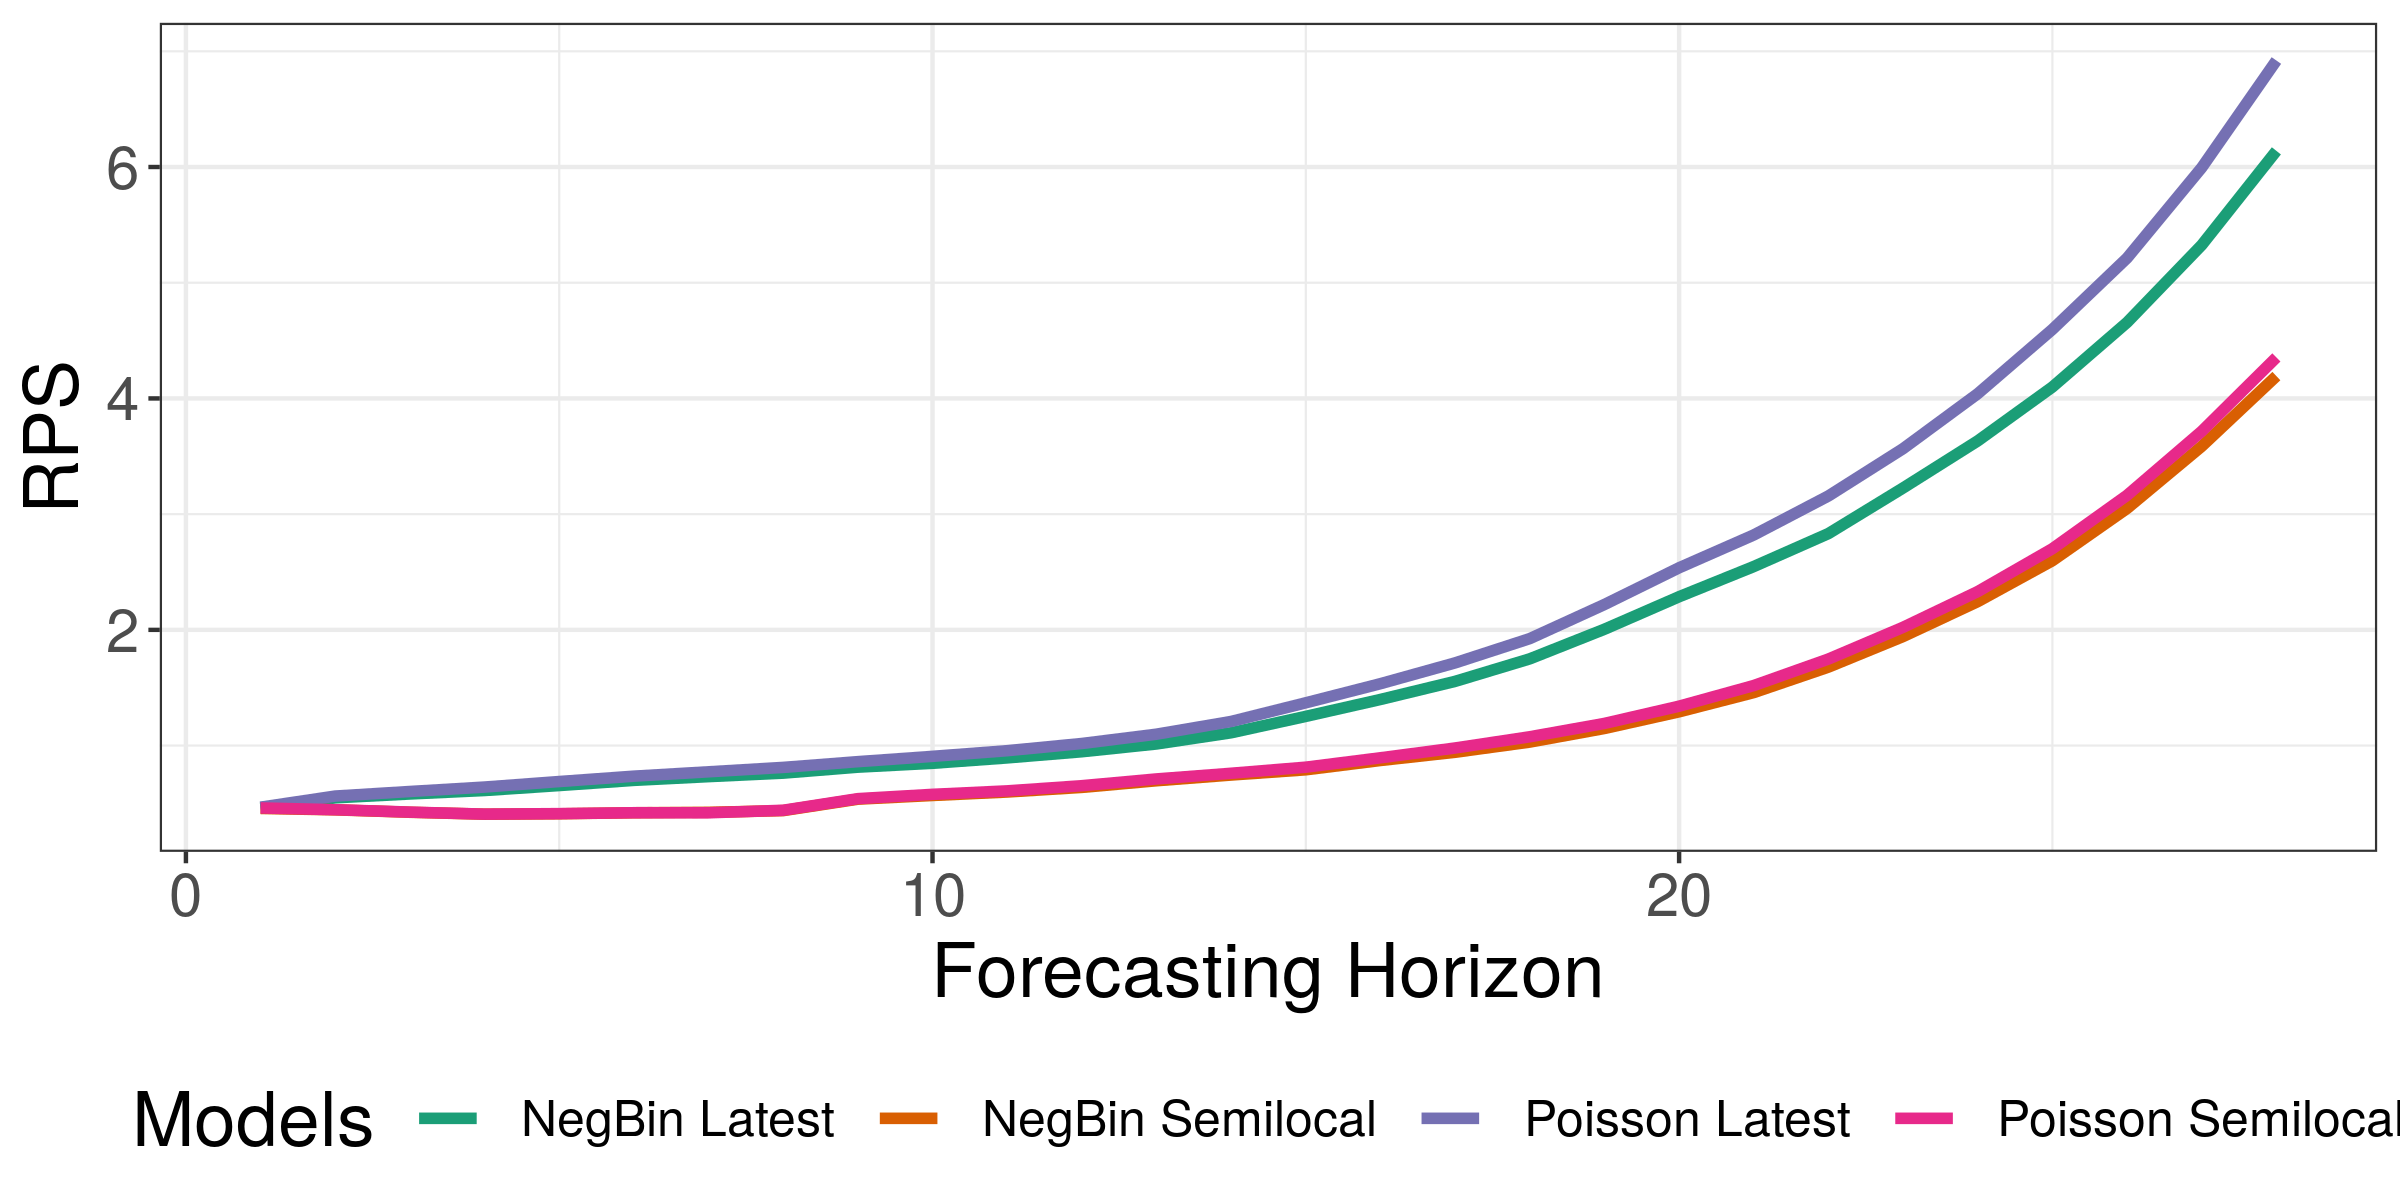
\includegraphics[width=\linewidth]{../output/Mabalako_crps.png}  
  \caption{Contineously Ranked Probability Score}
  \label{Mabalako_scores_1}
\end{subfigure}
\begin{subfigure}{0.5\textwidth}
  \centering
  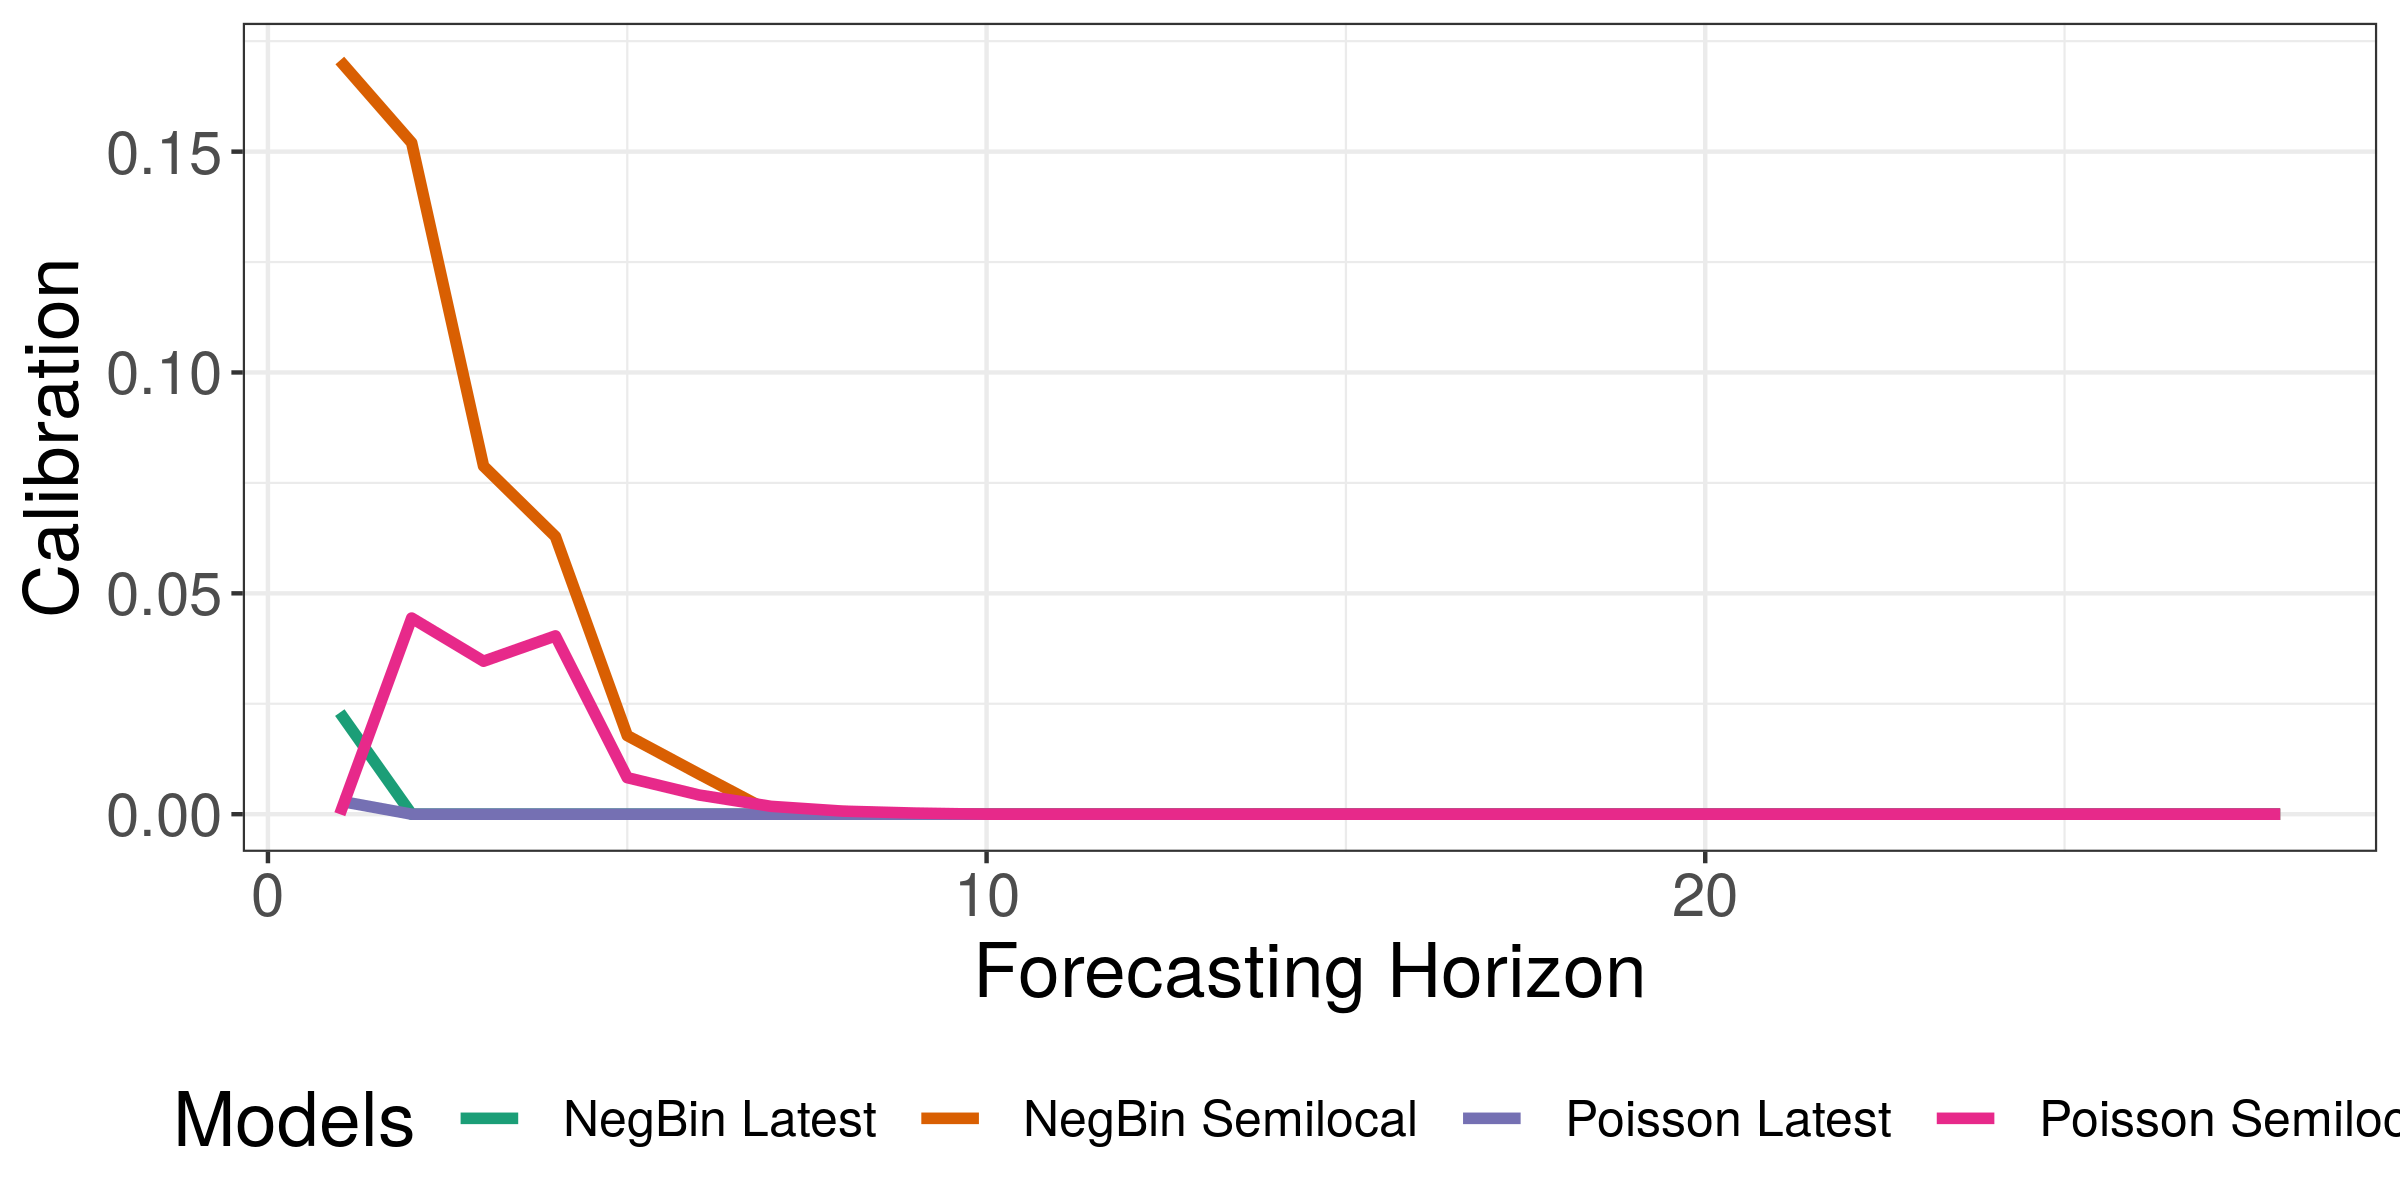
\includegraphics[width=\linewidth]{../output/Mabalako_calibration.png}  
  \caption{Calibration p-value}
  \label{Mabalako_scores_2}
\end{subfigure}

\begin{subfigure}{0.5\textwidth}
  \centering
  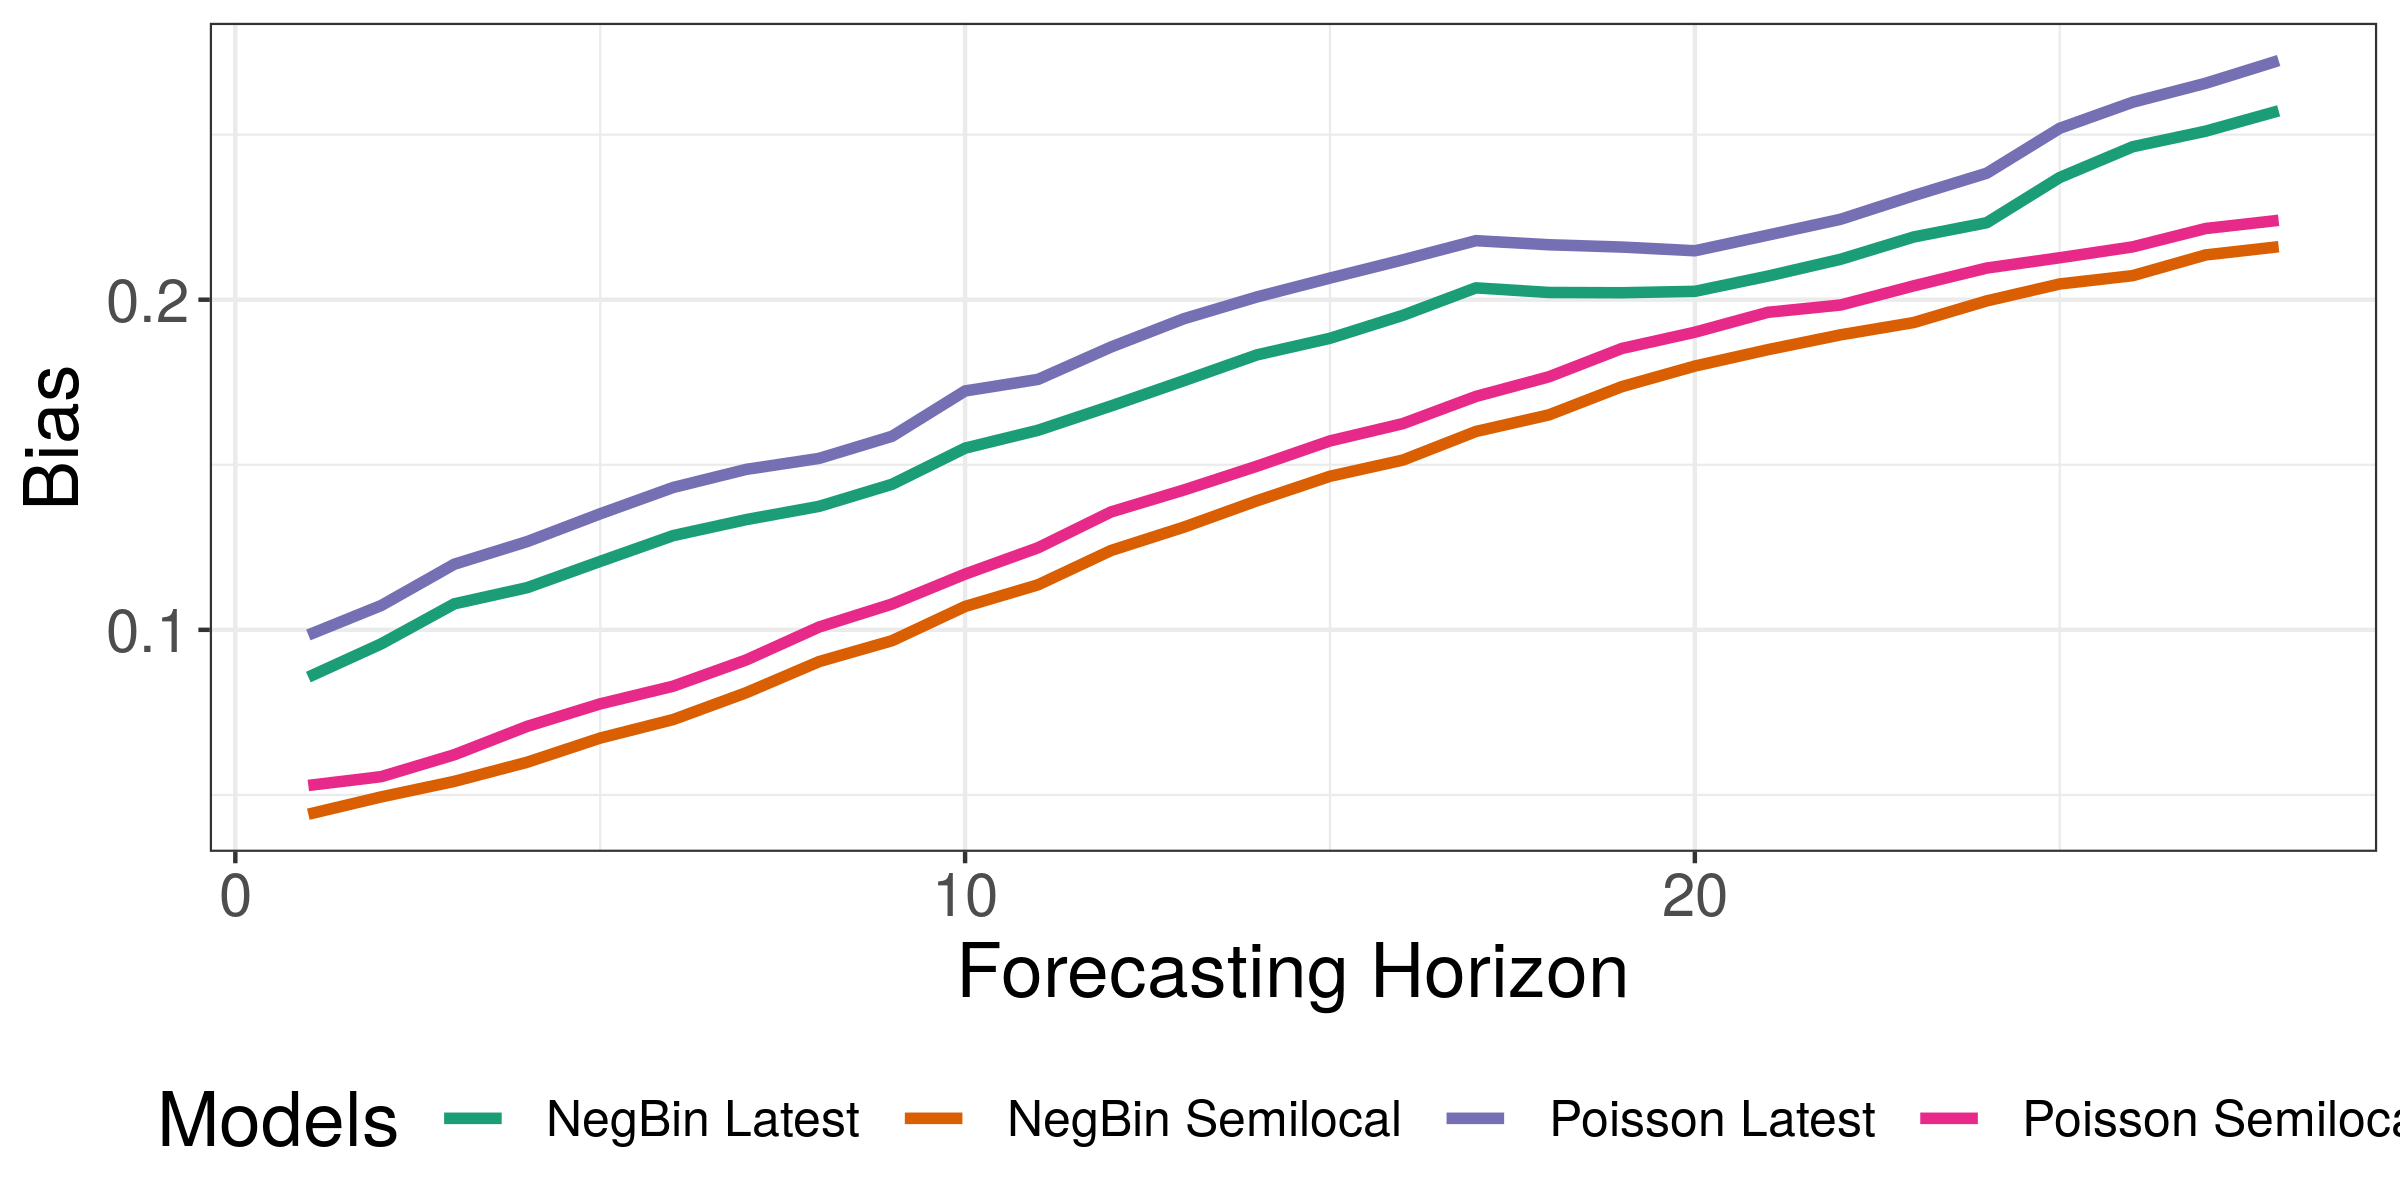
\includegraphics[width=\linewidth]{../output/Mabalako_bias.png}  
  \caption{Bias}
  \label{fig:Mabalako_scores_3}
\end{subfigure}
\begin{subfigure}{0.5\textwidth}
  \centering
  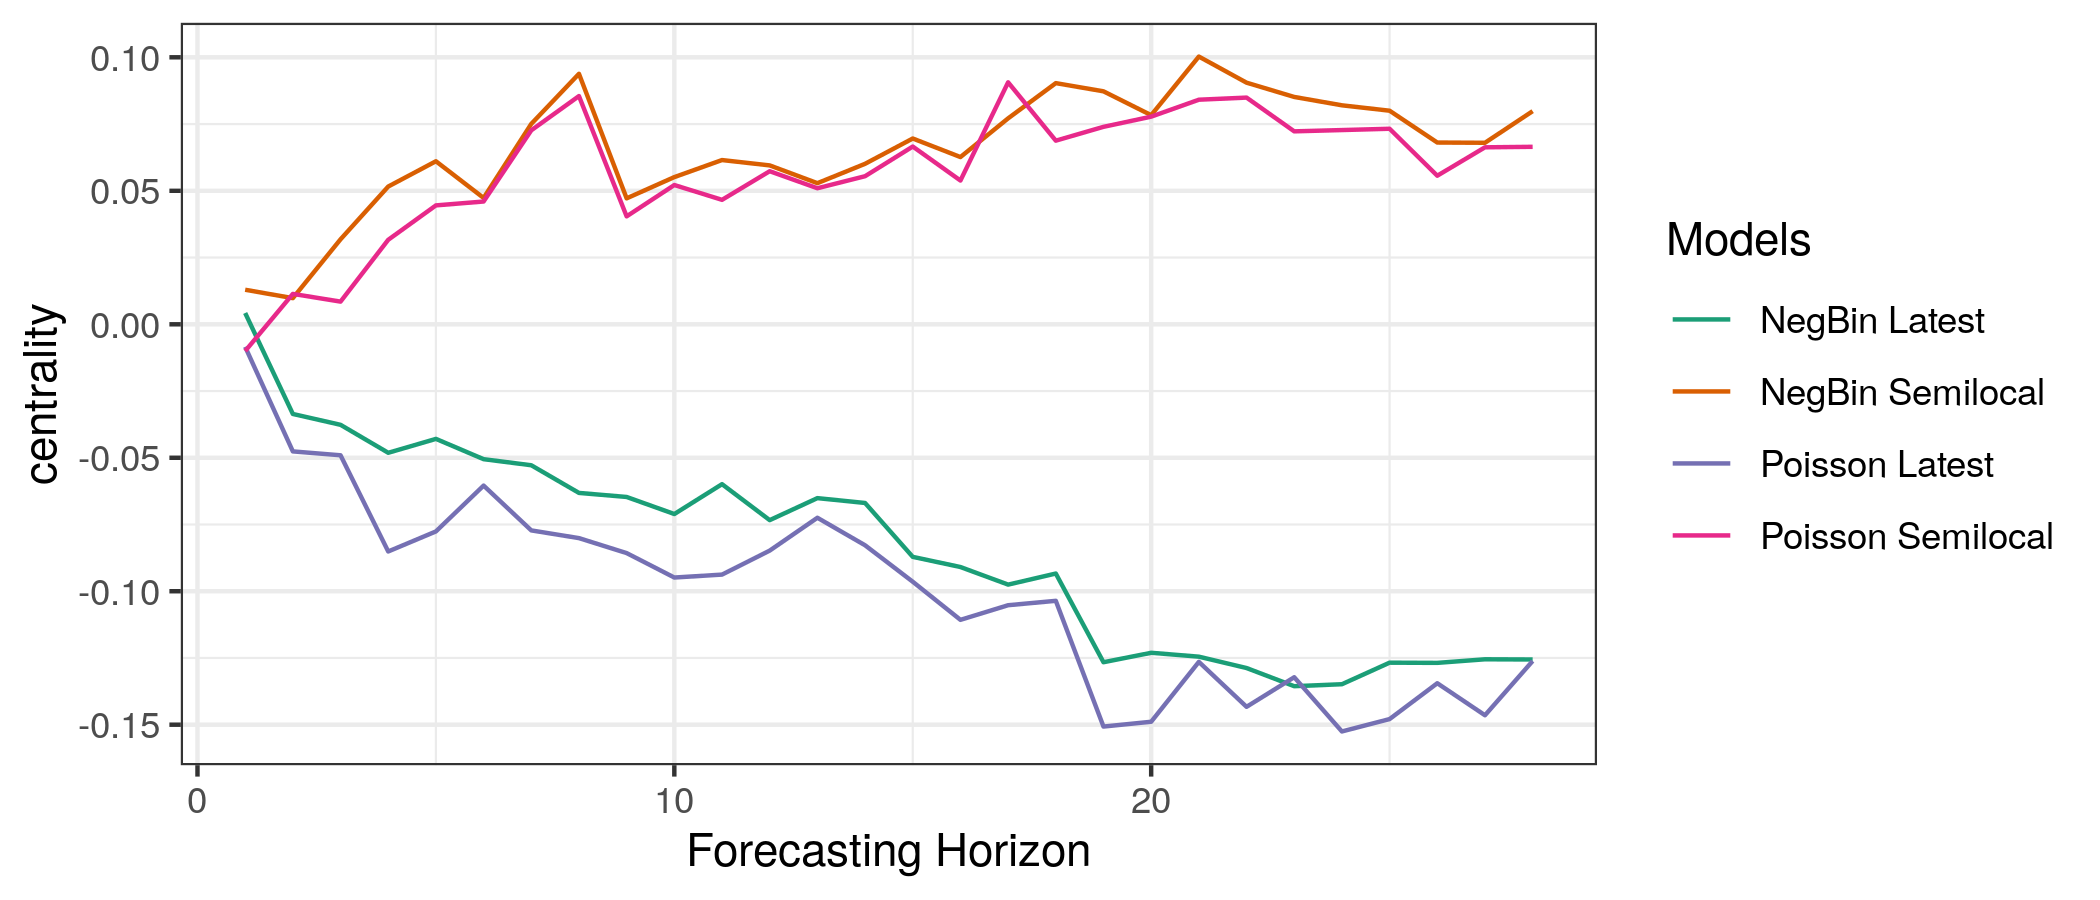
\includegraphics[width=\linewidth]{../output/Mabalako_centrality.png}  
  \caption{Centrality of PIT values}
  \label{fig:Mabalako_scores_4}
\end{subfigure}
  \caption{Scores for Mabalako as a function of the forecasting horizon.}

  \label{fig:nat_scores}
\end{figure}
 \section{ Tchomia }\begin{figure}[H]\begin{subfigure}{\textwidth}  \centering  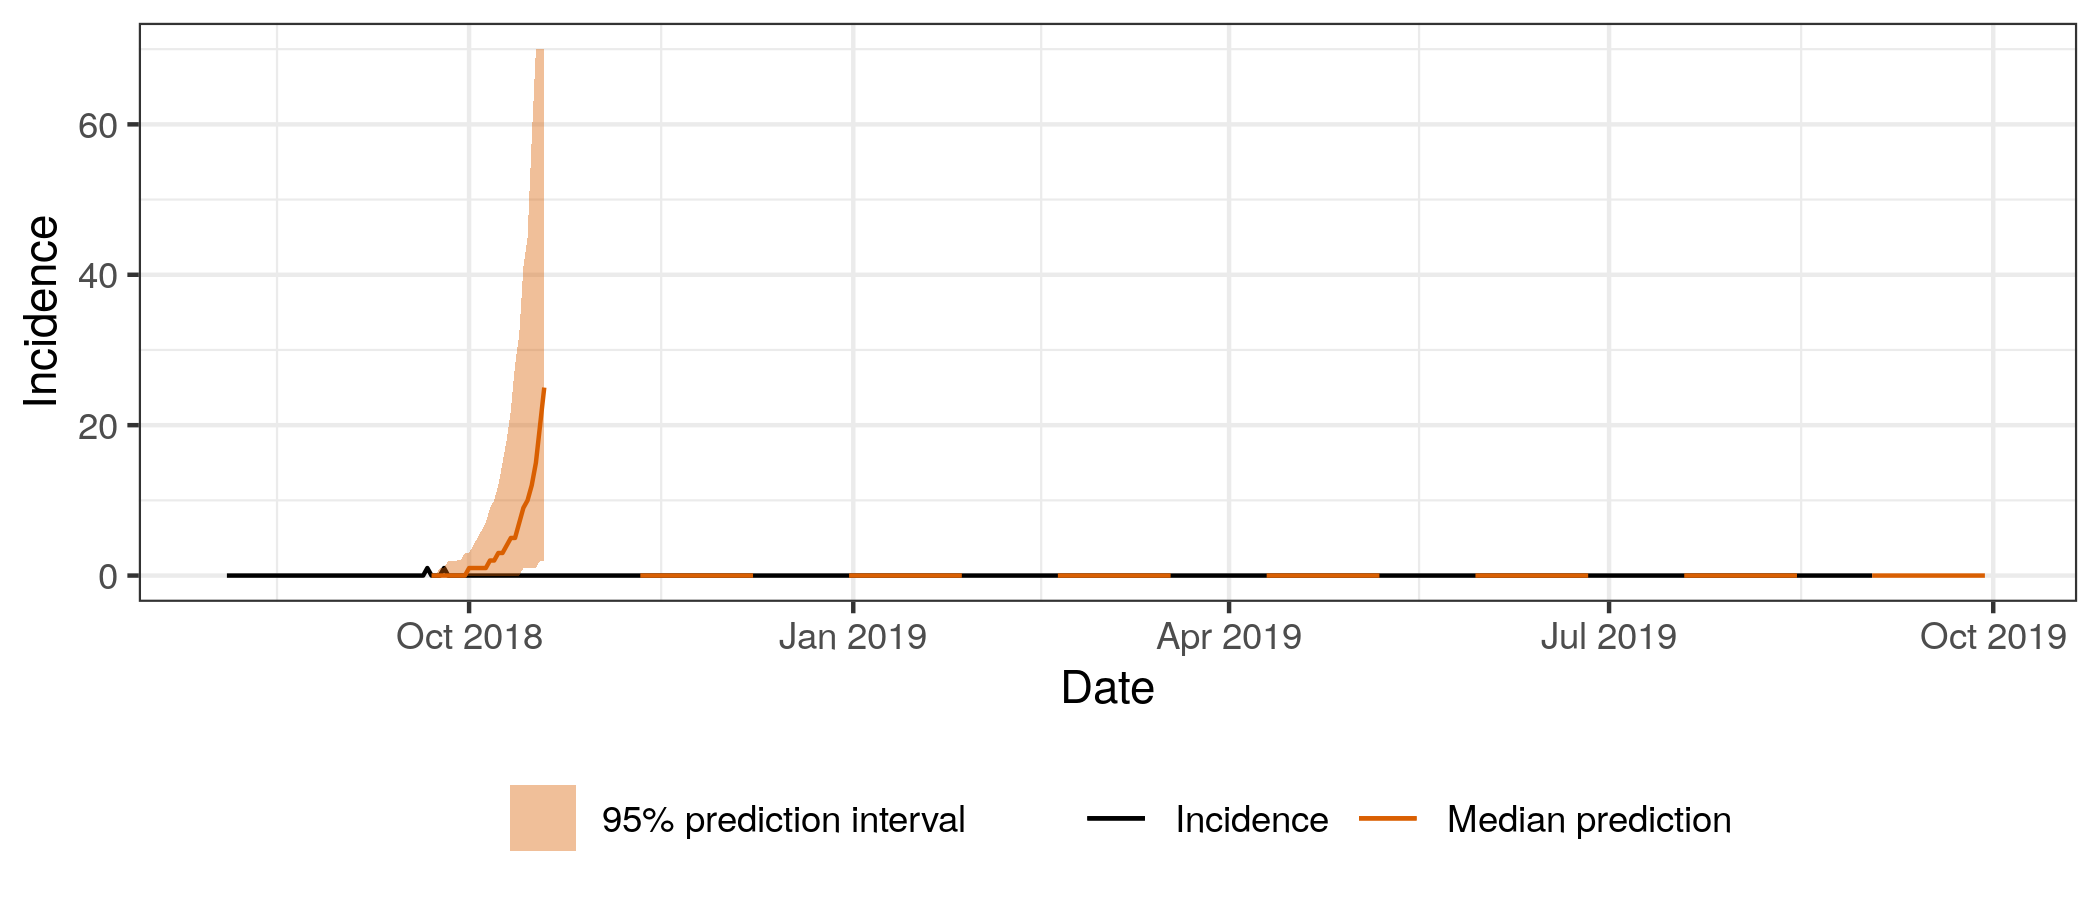
\includegraphics[width=0.9\linewidth, height=7cm]{../output/Tchomia_predictions.png}  \caption{Forecasted and predicted incidence for the best fitting model}\end{subfigure}

\begin{subfigure}{\textwidth}  \centering  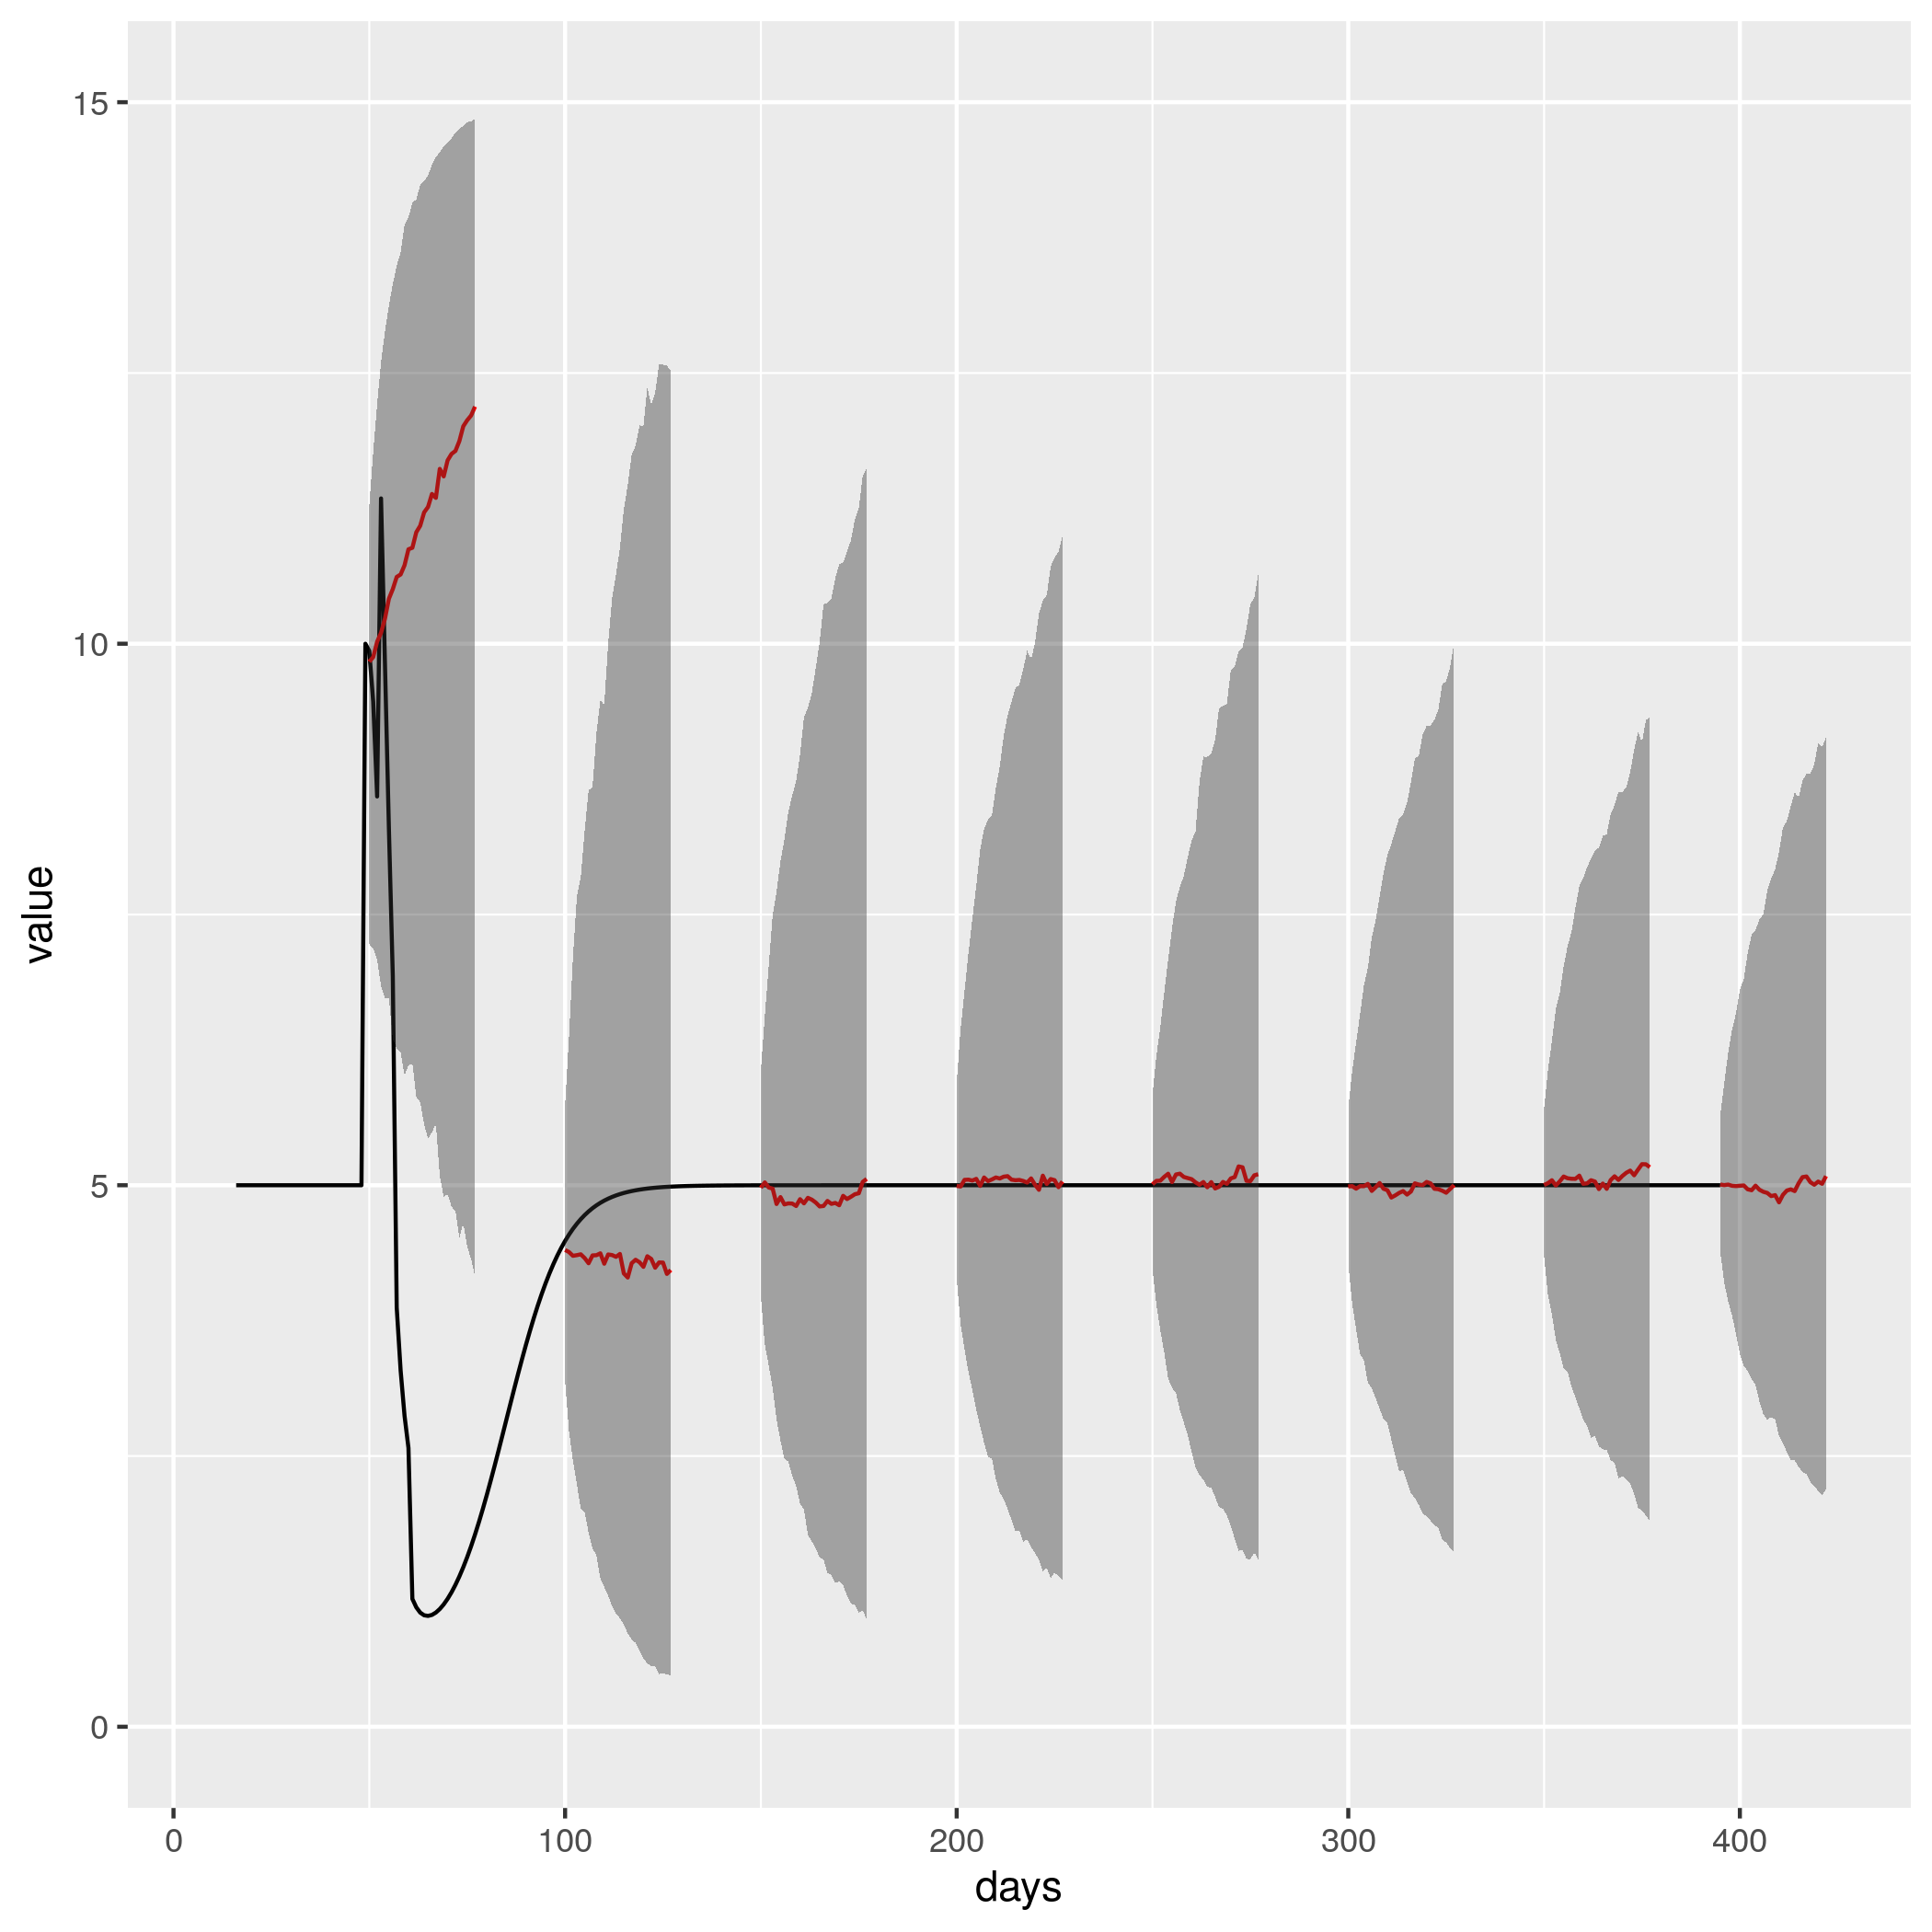
\includegraphics[width=0.9\linewidth, height=7cm]{../output/Tchomia_Rs.png}  \caption{Forecasted and predicted repreoduction numbers for the best fitting model}\end{subfigure}  \caption{Median forecast with 95 \% prediction intervals and observed values for incidence and reproduction number for the best fitting model for Tchomia.}\end{figure}

\begin{figure}[H]
\begin{subfigure}{0.5\textwidth}
  \centering
  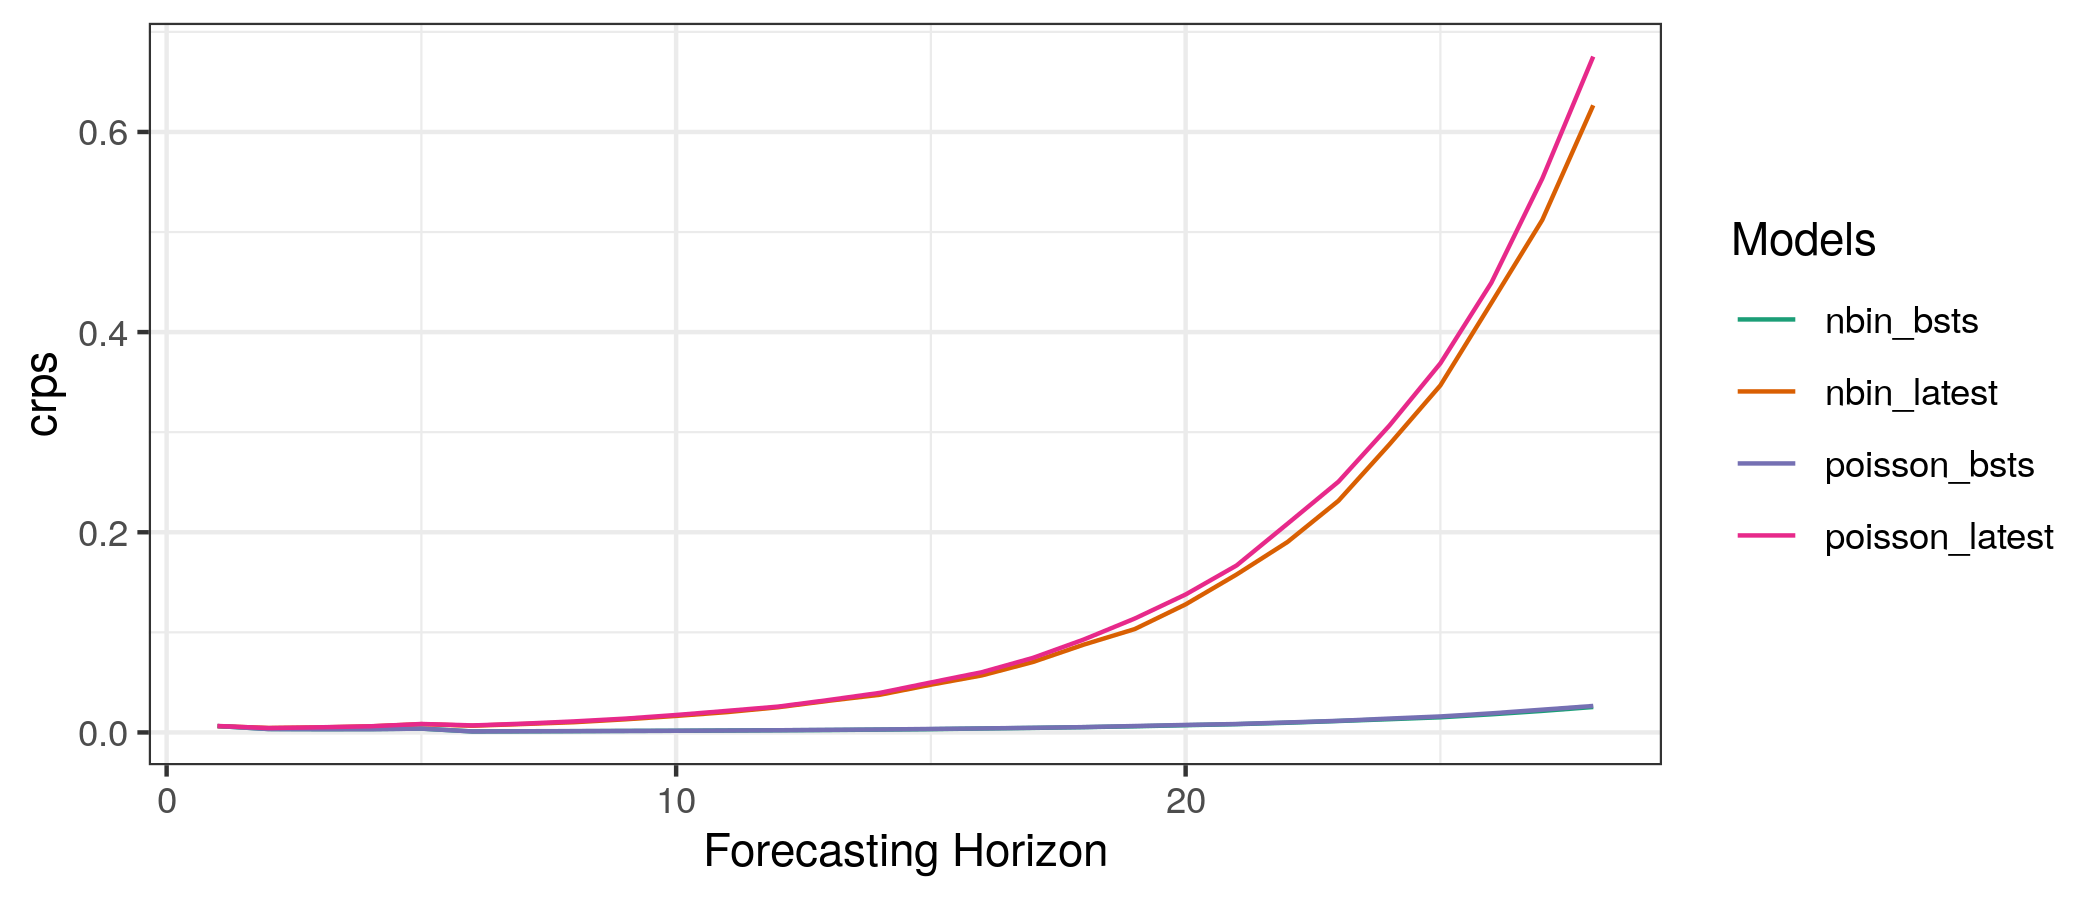
\includegraphics[width=\linewidth]{../output/Tchomia_crps.png}  
  \caption{Contineously Ranked Probability Score}
  \label{Tchomia_scores_1}
\end{subfigure}
\begin{subfigure}{0.5\textwidth}
  \centering
  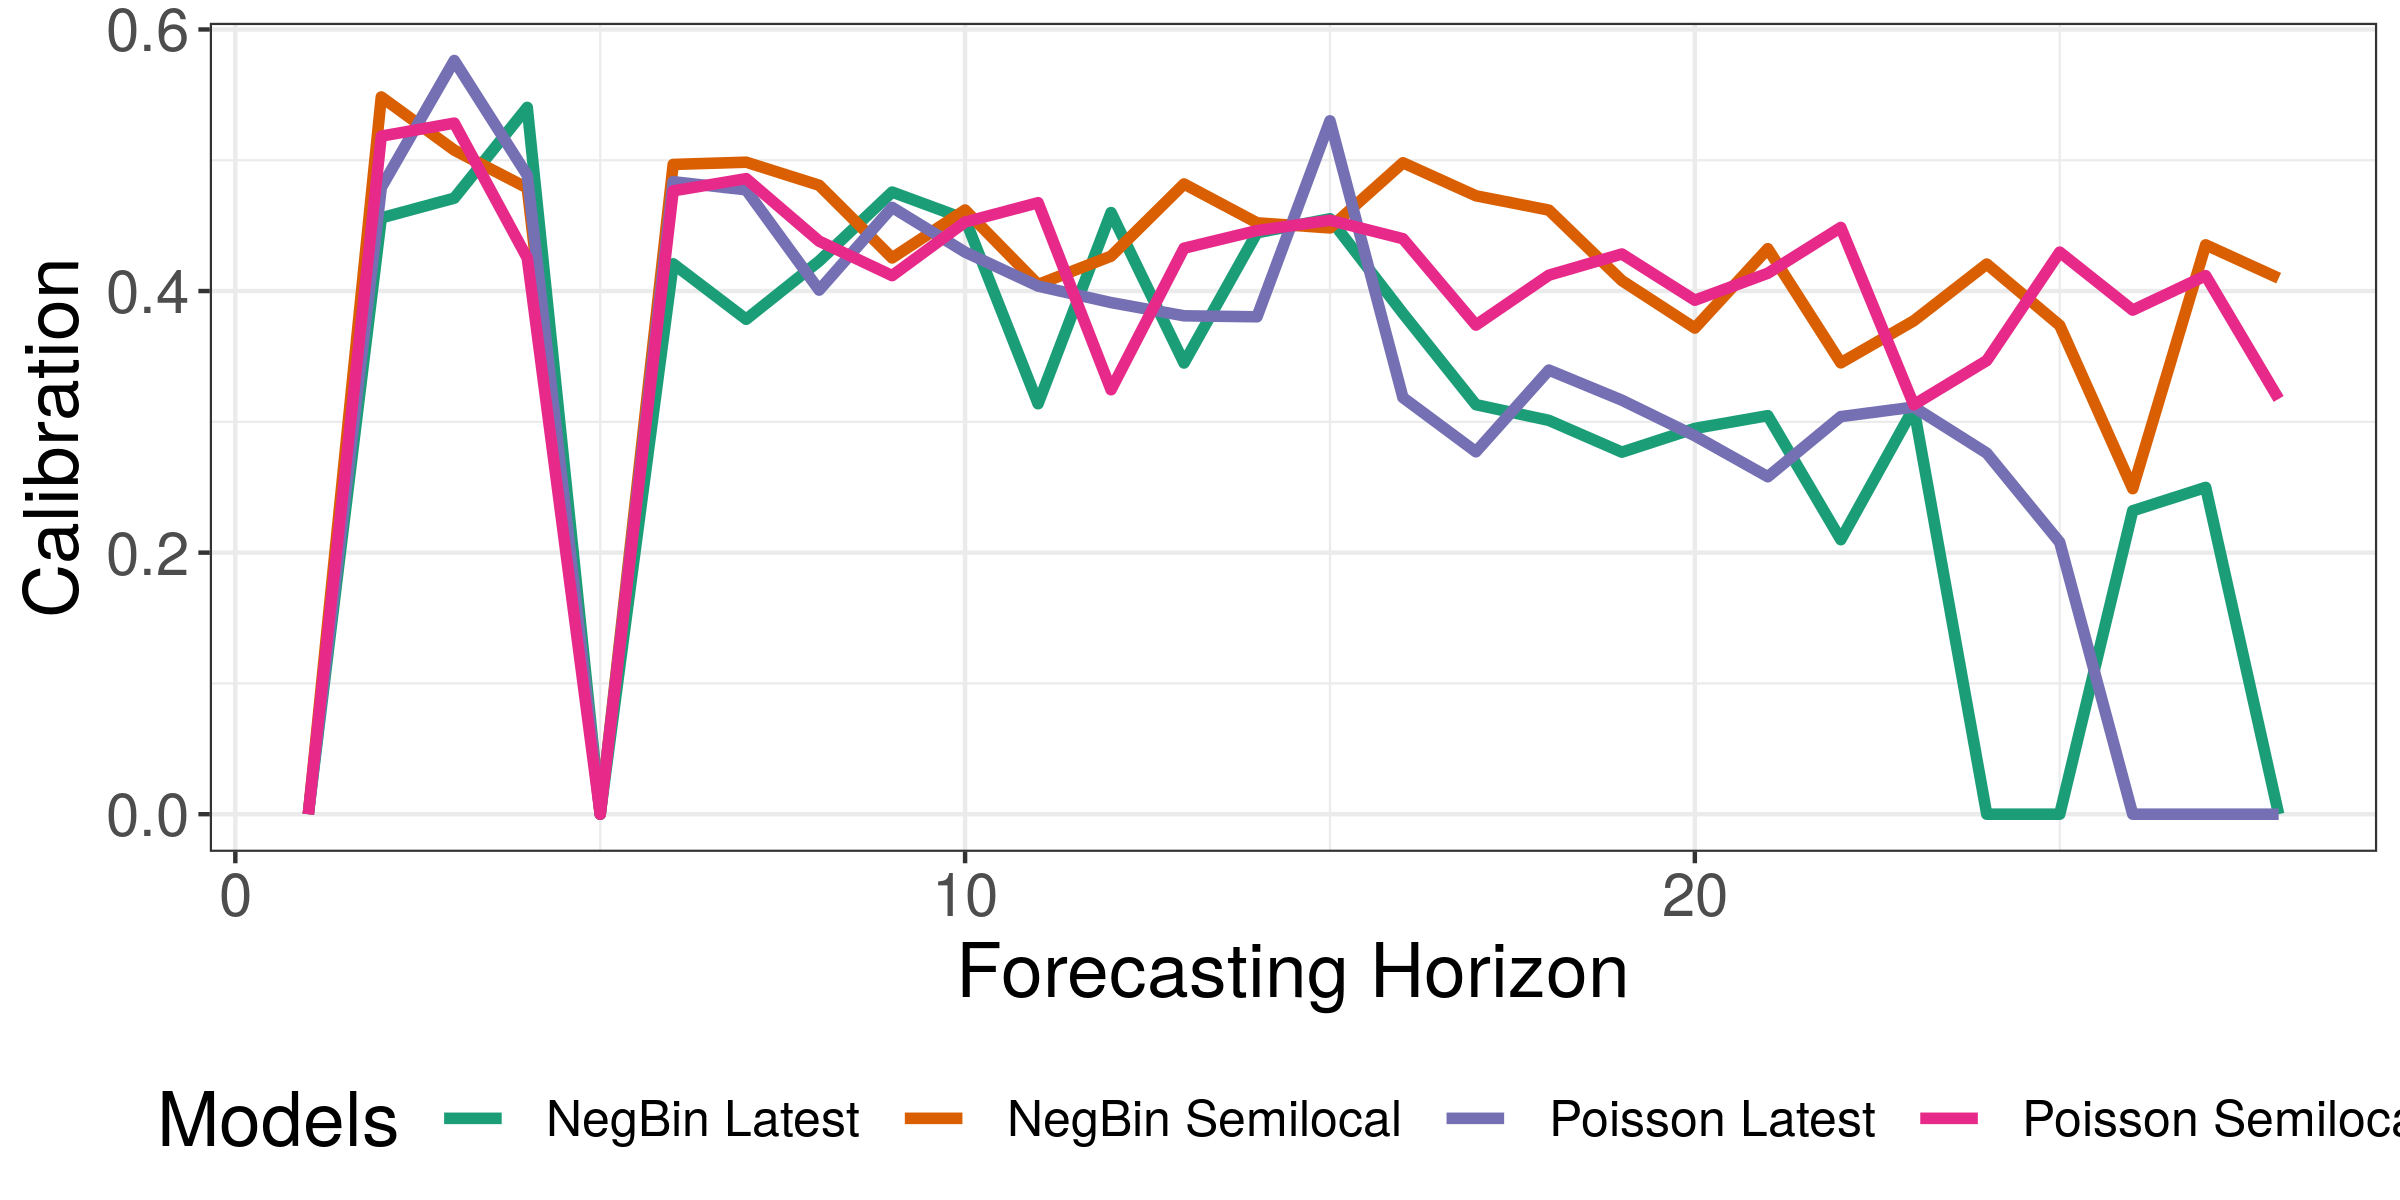
\includegraphics[width=\linewidth]{../output/Tchomia_calibration.png}  
  \caption{Calibration p-value}
  \label{Tchomia_scores_2}
\end{subfigure}

\begin{subfigure}{0.5\textwidth}
  \centering
  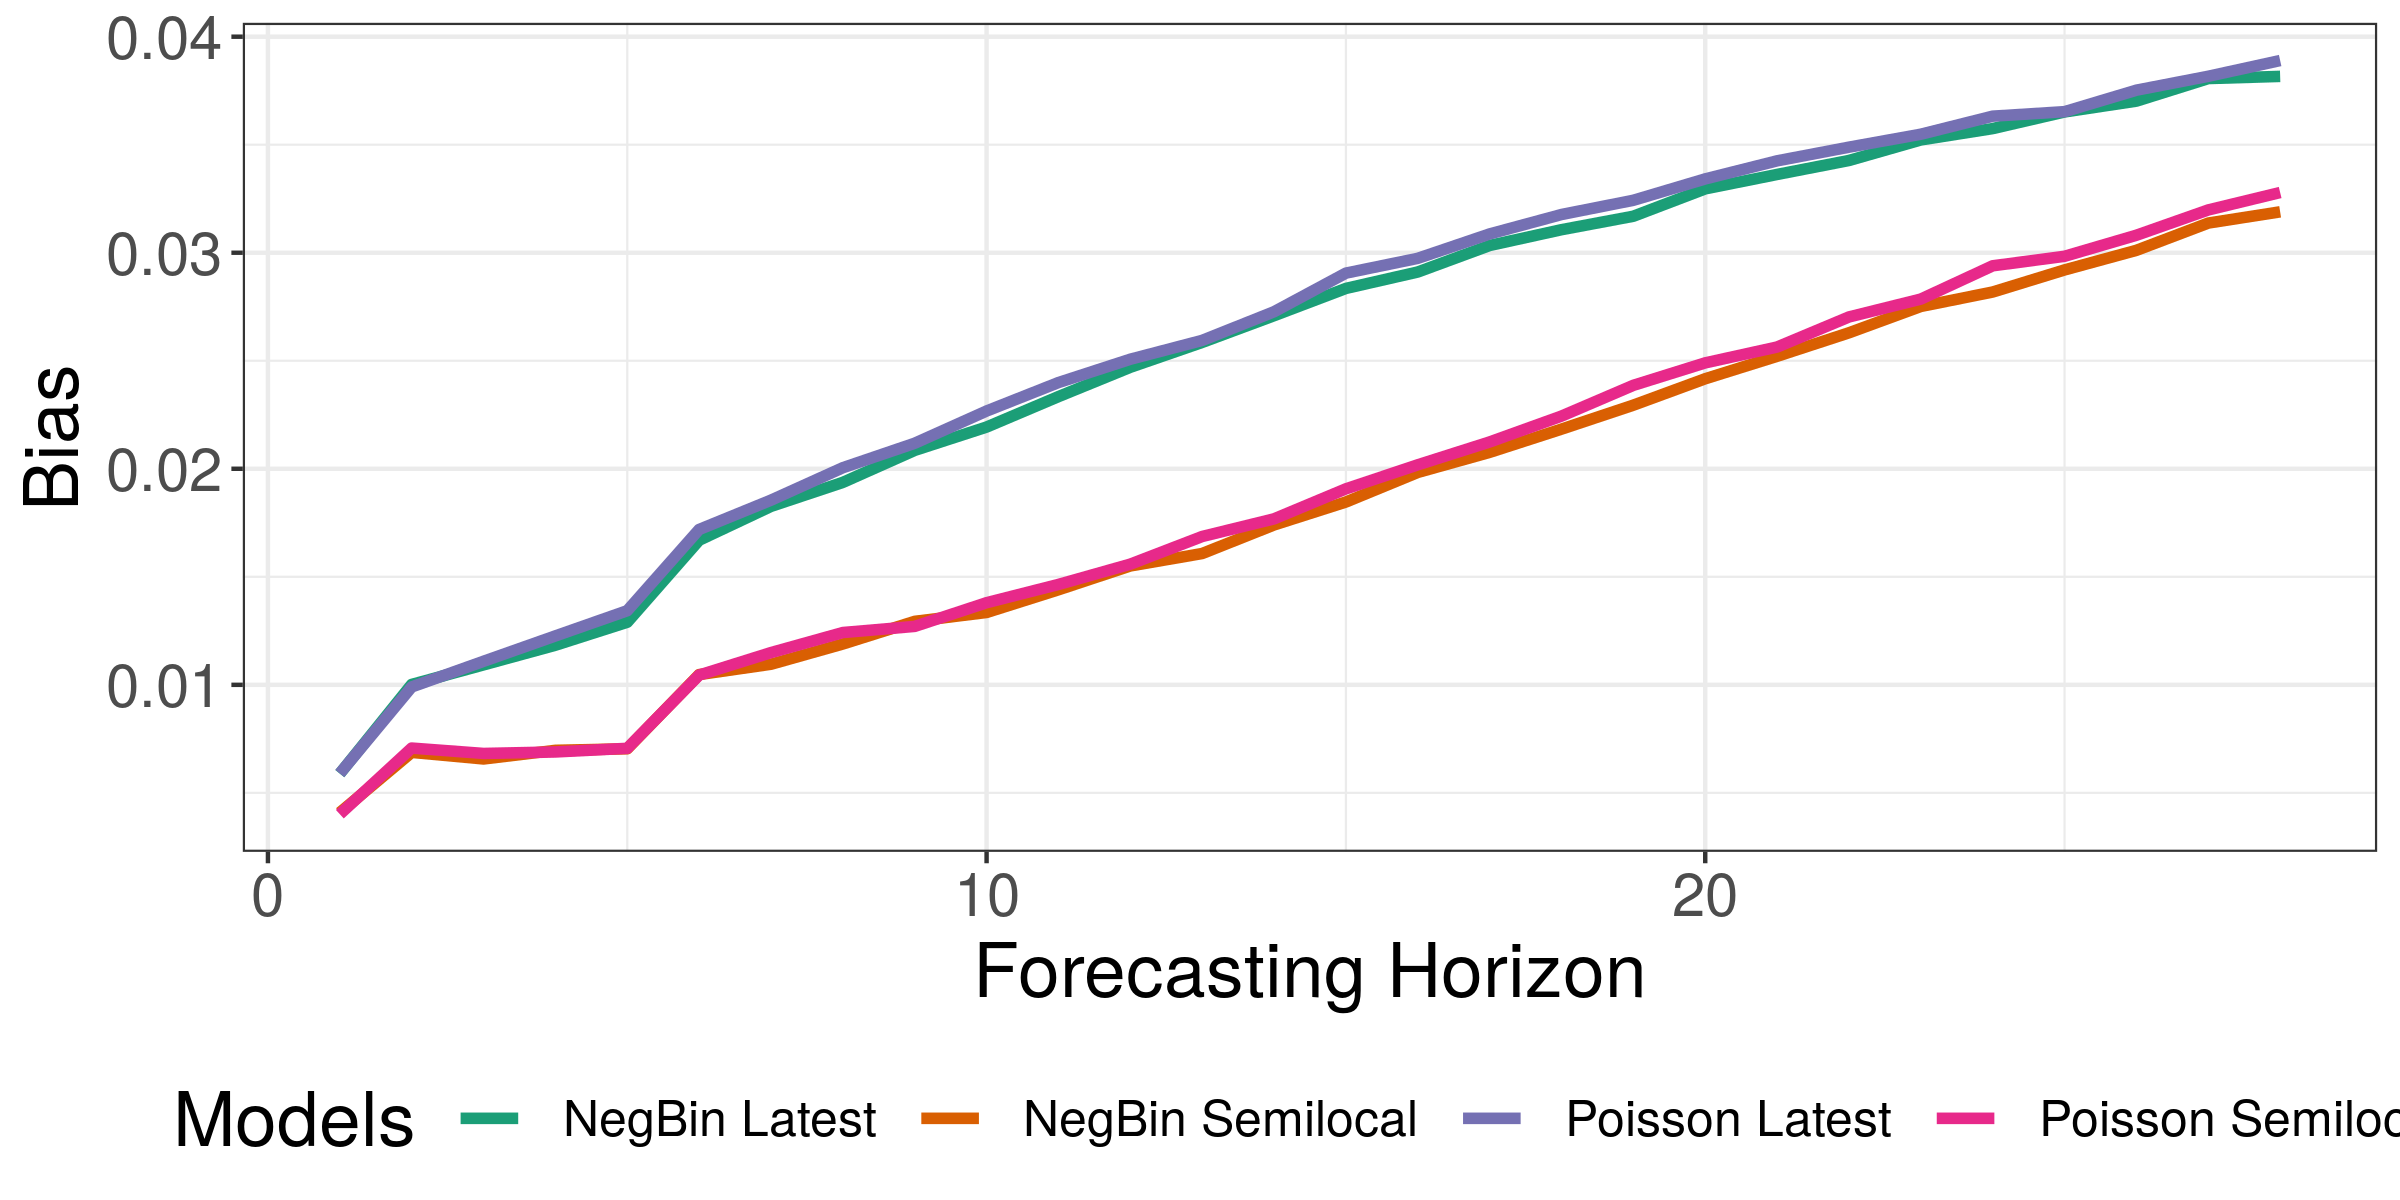
\includegraphics[width=\linewidth]{../output/Tchomia_bias.png}  
  \caption{Bias}
  \label{fig:Tchomia_scores_3}
\end{subfigure}
\begin{subfigure}{0.5\textwidth}
  \centering
  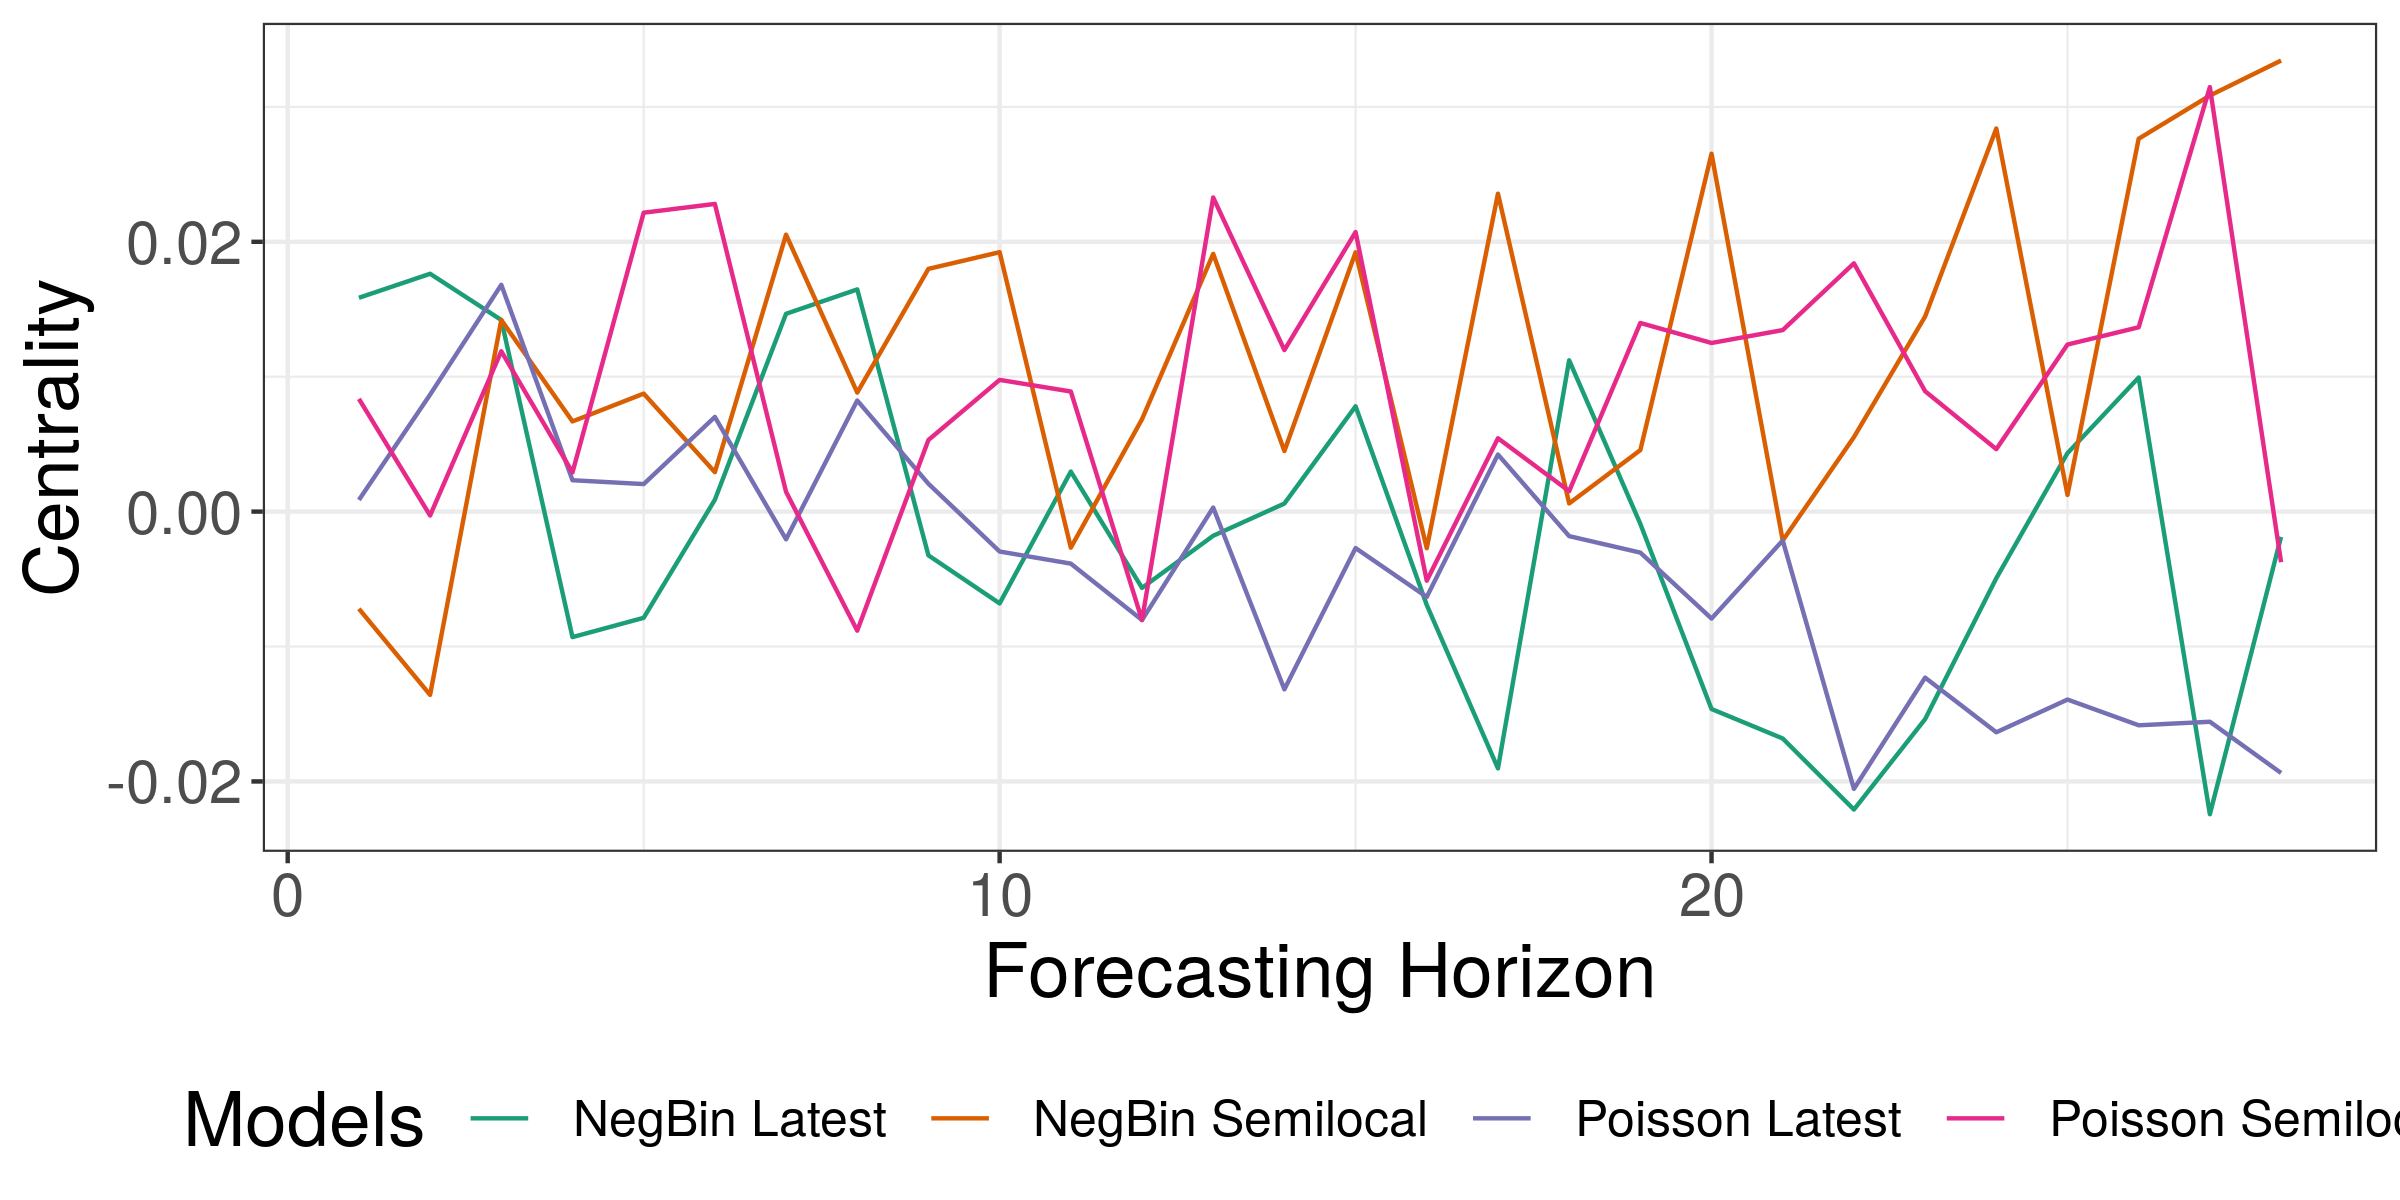
\includegraphics[width=\linewidth]{../output/Tchomia_centrality.png}  
  \caption{Centrality of PIT values}
  \label{fig:Tchomia_scores_4}
\end{subfigure}
  \caption{Scores for Tchomia as a function of the forecasting horizon.}

  \label{fig:nat_scores}
\end{figure}



\end{document}
